\documentclass[12pt]{mathesisclass}
\setlength\parindent{0pt}


%load any additional packages
\usepackage{amssymb,amsfonts}
\usepackage[all,arc]{xy}
\usepackage{paralist}
\usepackage[shortlabels]{enumitem}
\setlist[enumerate]{topsep=0pt, leftmargin=*, itemsep=0pt, parsep=0pt}
\usepackage{amsthm}
\usepackage{amsmath, amscd}
\usepackage{mathtools}
\usepackage{mathrsfs}
\usepackage{xspace}
\usepackage{amscd}
\usepackage[latin2,utf8]{inputenc}
\usepackage{t1enc}
\usepackage[mathscr]{eucal}
\usepackage{indentfirst}
\usepackage{graphicx}
\usepackage{graphics}
\usepackage{pict2e}
\usepackage{epic}
\usepackage{MnSymbol}
\numberwithin{equation}{section}
\usepackage[margin=2.9cm]{geometry}
\usepackage{epstopdf} 
\usepackage{tensor}
\usepackage{scalerel}
\usepackage[tiny]{titlesec}
\usepackage{pdfpages}
%tikz
\usepackage{tikz-cd}
\usetikzlibrary{arrows,chains,matrix,positioning,scopes}
\makeatletter
\tikzset{join/.code=\tikzset{after node path={%
\ifx\tikzchainprevious\pgfutil@empty\else(\tikzchainprevious)%
edge[every join]#1(\tikzchaincurrent)\fi}}}
\makeatother
\tikzset{>=stealth',every on chain/.append style={join},
         every join/.style={->}}
\tikzstyle{labeled}=[execute at begin node=$\scriptstyle,
   execute at end node=$]


%
\def\numset#1{{\\mathbb #1}}
\theoremstyle{plain}
\newtheorem{theorem}{Theorem}[section]
\newtheorem{lemma}[theorem]{Lemma}
\newtheorem{cor}[theorem]{Corollary}
\newtheorem{prop}[theorem]{Proposition}


\theoremstyle{definition}
\newtheorem{definition}[theorem]{Definition}
\newtheorem{rem}[theorem]{Remark}
\newtheorem{ex}[theorem]{Example}



\newcommand{\im}{\operatorname{im}}
\newcommand{\imm}{\operatorname{Im}}
\newcommand{\Hom}{{\rm{Hom}}}
\newcommand{\Ker}{{\rm{ker}}}
\newcommand{\Coker}{{\rm{coker}}}
\newcommand{\h}[1]{{h_{#1}}}
\newcommand{\Id}{{\rm{Id}}}
\newcommand{\Gal}{{\rm{Gal}}}
\newcommand{\pione}{\pi_1}
%\newcommand{\norm}[1]{\abs{#1}}
\newcommand{\norm}[1]{\lvert#1\rvert}
\newcommand{\normx}[1]{\norm{#1}_{x}}
\newcommand{\spec}[1]{{Spec{\:#1}}}
\newcommand{\specc}[1]{{Spec({\:#1})}}
\newcommand{\cont}[1]{{\mathrm{Cont}(#1)}}     		%%%custom
\newcommand{\spf}[1]{{Spf{\:#1}}}
\newcommand{\spff}[1]{{Spf({\:#1})}}
\newcommand{\spa}[2]{{Spa({#1},{#2})}}     		%%%customx
\newcommand{\spaa}[1]{{Spa{\:#1}}}     		%%%customx
\newcommand{\upcirc}{{^{\circ}}}
\newcommand{\upcirca}{{^{\circ a}}}
\newcommand{\upplus}{{^{+}}}
\newcommand{\twocirc}{^{\circ\circ}}
\newcommand{\tilt}{^{\flat}}
\newcommand{\normxtilt}[1]{\norm{#1}_{x\tilt}}
\newcommand{\shrp}{^{\#}}
\newcommand{\tiltshrp}{^{\flat\#}}
\newcommand{\lowcirc}{{_{\circ}}}
\newcommand{\ovl}{\overline}
\newcommand{\slfrac}[2]{\left.#1\middle/#2\right.} %% Slash fraction
\newcommand{\ctens}{\mathbin{\hat{\otimes}}}
\newcommand{\tens}{\mathbin{\otimes}}
\newcommand{\catname}[1]{\mathbf{#1}}

%  notations %
\newcommand{\perfc}{\mathrm{Perf}_{C}}
\newcommand{\perfctilt}{\mathrm{Perf}_{C\tilt}}
\newcommand{\perfcsite}{\mathrm{Perf}_{C}^{pro-\acute{e}t}}
\newcommand{\shvperfc}{\mathbf{Shv}(\mathrm{Perf}_{C}^{pro-\acute{e}t})}
\newcommand{\pu}{\varpi}
\newcommand{\Q}{\mathbb{Q}}
\newcommand{\Qp}{\mathbb{Q}_p}
\newcommand{\Fp}{\mathbb{F}_p}
\newcommand{\Fq}{\mathbb{F}_q}
\newcommand{\Zp}{\mathbb{Z}_p}
\newcommand{\R}{\mathbb{R}}
\newcommand{\C}{\mathbb{C}}
\newcommand{\Z}{\mathbb{Z}}
\newcommand{\N}{\mathbb{N}}
\newcommand{\Oo}{\mathcal{O}}
\newcommand{\F}{\mathcal{F}}
\newcommand{\D}{\mathcal{D}}
\newcommand{\G}{\mathcal{G}}
\newcommand{\Hh}{\mathcal{H}}
\newcommand{\X}{\mathcal{X}}
\newcommand{\Y}{\mathcal{Y}}
\newcommand{\E}{\mathcal{E}}
\DeclareMathOperator{\End}{End}
\DeclareMathOperator{\id}{id}

\newcommand\restr[2]{{% we make the whole thing an ordinary symbol
  \left.\kern-\nulldelimiterspace % automatically resize the bar with \right
  #1 % the function
  \vphantom{|} 
  \right|_{#2} % this is the delimiter
  }}




\title{The absolute Galois group of $\Qp$ as\\[1ex]    
        \'{e}tale fundamental group of a \\[1ex]    
	diamond}   


\author{Amr Umeri}             


\degree{MSc Mathematics ETHZ}     
\degreedate{2021}        


\begin{document}

%this baselineskip gives sufficient line spacing
\baselineskip=18pt plus1pt

%set the number of sectioning levels that get number and appear in the contents
\setcounter{secnumdepth}{3}
\setcounter{tocdepth}{2}


\maketitle                 				
\newpage\null\thispagestyle{empty}\newpage
\begin{acknowledgements}
I would like to thank Joseph Ayoub for suggesting me this topic, which perfectly matched my taste in mathematics. I would like to thank also Özlem Imamoglu for  administrating this thesis at ETH Zurich and for her introductory lectures on number theory. Many concepts which found their way in this thesis I have encountered first in the lecture on \emph{p-adic Galois representations} offered by Maxim Mornev in autumn 2019 at ETH Zurich, for which I am very grateful. I did benefit also from the Zoom-lecture on the \emph{geometrization of the local Langlands correspondence} offered by Peter Scholze in 2020. Finally I would like to thank Jared Weinstein, the author of the paper on which this thesis is based, for the discussions via e-mail  and Bianca Morrone for reading a preliminary version of this thesis. 
\end{acknowledgements}
       
\newpage\null\thispagestyle{empty}\newpage 
%\thispagestyle{empty}
\begin{center}
\emph{In memory of my mother.}
\end{center}        
%\newpage\null\thispagestyle{empty}\newpage

\begin{abstract}
Fix a prime number $p$ and let $E$ be a finite extension of the $p$-adic numbers $\Qp$.
We study the \emph{perfectoid open unit disk} over an algebraically closed non-Archimedean extension $C$ of $E$. We denote by $\perfc$ the category of perfectoid spaces over $\spa{C}{\Oo_C}$. The disk parametrizes topologically nilpotent elements of the tilt of a perfectoid ring over $C$ and can be understood as a replacement of the affine line in algebraic geometry.\footnote{This is a strong claim.} In fact the perfectoid open unit disk is an $E$-vector space object in the categroy $\perfc$.  By removing certain points of the unit disk we get the \emph{punctured perfectoid open unit disk} which is representable as a perfectoid space and is related to the \emph{adic Fargues-Fontaine curve} via the \emph{tilting equivalence}. The classification of vector bundles on the adic Fargues-Fontaine curve will show that heuristically the curve is a geometrization of $\spec{E}$. There is a quotient of the punctured disk which exists as a \emph{diamond} and whose \'{e}tale fundamental group is the \'{e}tale fundamental group of $\spec{E}$. The entire thesis is based on Jared Weinstein's paper \cite{Weinstein16}. The exposition deviates in many parts from the original reference.% and is self-contained.





\end{abstract}    
\newpage\null\thispagestyle{empty}\newpage
\begin{romanpages}      						
\tableofcontents
\newpage\null\thispagestyle{empty}\newpage
\end{romanpages}     
    


\chapter{Adic spaces}
Rings are commutative and have a unit. Complete topological rings are always assumed to be separated.
We introduce \emph{adic spaces}, which is a class of locally ringed spaces.
First we introduce \emph{Huber rings}, \emph{Huber-Tate pairs} and \emph{adic spectra}. A topological ring is called \emph{Huber} if it contains an open subring which is adic for a finitely generated ideal of definition. The original references are \cite{Huber93} and \cite{Huber94}. %Expositions are given in \cite{Morel19}, \cite{SW20}.


\section{Continuous valuation spectrum}
We define the set of continuous valuations on a topological ring. Under an identification, the continuous valuations on the ring form the points of the so-called
\emph{continuous valuation spectrum}.\\

Let $\Gamma$ denote a totally ordered multiplicative abelian group. We write $\Gamma\cup\{0\}$ for the group with some element adjoined and we extend the total order relation and the multiplication to this set by requiring that
 $0<\gamma$ and $0\gamma = \gamma0 =  0$ for all $\gamma\in\Gamma$.

\begin{definition}
Let $A$ be a ring.
A (multiplicative) \emph{valuation} on $A$ is a map
\[\norm{\cdot}\colon A\to\Gamma\cup\{0\}\]
satisfying the following properties:
\begin{enumerate}
\item $\norm{0}=0$, $\norm{1}=1$,
\item $\forall a,b\in A$, $\norm{ab}=\norm{a}\norm{b}$,
\item $\forall a,b\in A$, $\norm{a+b}\leq\max\{\norm{a},\norm{b}\}$.
\end{enumerate}
\vspace{2mm}
The \emph{value group} of a valuation $\norm{\cdot}\colon A\to\Gamma\cup\{0\}$ is the subgroup of $\Gamma$ generated by $\Gamma\cap\norm{A}$.
It will be denoted by $\Gamma_{\norm{\cdot}}$ henceforth. The valuation will be called trivial if $\Gamma_{\norm{\cdot}}=\{1\}$. 
\end{definition}

Notice that the kernel of a valuation $\norm{\cdot}\colon A\to\Gamma\cup\{0\}$, $\ker{\norm{\cdot}}=\{a\in A \:\vert \:\norm{a}=0\}$,   is a prime ideal of $A$. 
Conversely, every prime ideal $\mathfrak{p}\subset A$ gives rise to a trivial valuation on $A$ with kernel $\mathfrak{p}\subset A$.\\

%Consider the following definition:
\begin{definition}
Let $A$ be a ring.
Consider the valuations on $A$,
$\norm{\cdot}_{1}\colon A\to\Gamma_{1}\cup\{0\}$ and 
$\norm{\cdot}_{2}\colon A\to\Gamma_{2}\cup\{0\}$
with value groups 
$\Gamma_{{\norm{\cdot}}_{1}}$, $\Gamma_{{\norm{\cdot}}_{2}}$.
We say that the valuations are \emph{equivalent} if there exists an order-preserving group isomorphism $\varphi\colon\Gamma_{{\norm{\cdot}}_{1}}\xrightarrow{\sim}\Gamma_{{\norm{\cdot}}_{2}}$
with $\varphi\circ{\norm{\cdot}}_{1} = {\norm{\cdot}}_{2}$. We extend the map by requiring $\varphi(0)=0$.
\end{definition}


Valuations define topologies on $A$ in an evident manner. We give the following definition to motivate \emph{continuous valuations}.

\begin{definition}
Let $A$ be a ring and let $\norm{\cdot}\colon A\to\Gamma\cup\{0\}$ be a valuation on $A$. Then the valuation defines a topology on $A$, the \emph{valuation topology},
by declaring a fundamental basis of open subsets around $0$ to be $\{a\in A\:\vert\: \norm{a}<\gamma\}$ for $\gamma\in\Gamma$. This defines a ring topology on $A$.
\end{definition}
\begin{definition}
Let $A$ be a topological ring. Let $\norm{\cdot}\colon A\to\Gamma\cup\{0\}$ be a valuation on $A$. We say that the valuation is \emph{continuous} if for every $\gamma\in\Gamma$,
$\{a\in A\mid \norm{a}<\gamma\}\subseteq A$ is an open subset.
Hence a valuation is continuous if and only if the topology on $A$ is finer than the valuation topology on $A$.
$\cont{A}$ will denote the set of equivalence classes of continuous valuations on $A$. $\cont{A}$ is called the \emph{continuous valuation spectrum} of $A$.
\end{definition}

Let $A$ be a topological ring. For $x\in\cont{A}$ we write $\normx{\cdot}\colon A\to\Gamma\cup\{0\}$ for an arbitrary representative. 
Standard notations are $\mathfrak{p}_x=\ker{\normx{\cdot}}$ and $K_x=A_{\mathfrak{p}_x}/{\mathfrak{p}_x}A_{\mathfrak{p}_x}$ for the associated prime ideal and residue field respectively.
The point $x\in\cont{A}$ is called \emph{analytic} if $\mathfrak{p}_x\subseteq A$ is not open. 
%The point $x\in\cont{A}$ is non-analytic if and only if the quotient topology on $A/\mathfrak{p}_x$ is discrete. 
For any $x\in\cont{A}$ the induced valuation 
$\normx{\cdot}\colon A/\mathfrak{p}_x\to\Gamma\cup\{0\}$ is continuous when $A/\mathfrak{p}_x$ is given the quotient topology. 
By construction the valuation extends to the fraction field
$\normx{\cdot}\colon K_x\to\Gamma\cup\{0\}$. In general analytic points have much better properties than non-analytic points. For example one can show that
for a Huber ring $A$ and analytic point $x\in\cont{A}$ the valuation topology on $K_x$ coincides with the valuation topology coming from a \emph{non-Archimedean} valuation, i.e. $K_x$ is a \emph{non-Archimedean}
field. %This is in fact an equivalence. %, since discrete topologies come from trivial valuations.
The completion of $K_x$ is denoted by $\kappa_x$ in the literature and is called the \emph{completed residue field} 
at $x\in\cont{A}$.
Many geometric objects that we will encounter in the upcoming chapters consist only of \emph{analytic} points. In fact removing non-analytic points of certain valuation spectra turns out to be a useful procedure to construct interesting geometric objects.\\

For certain topological rings $A$ one can topologize $\cont{A}$ such that it becomes a \emph{spectral space}.  %Equivalently it is homeomorphic to the Zariski-spectrum of a ring.% in particular it has a basis of quasi-compact open subsets. 
However this is not the approach taken when defining \emph{adic spaces}. Instead one requires additional properties on the ring $A$ and one is interested in certain subsets of $\cont{A}$.\\

Recall that the underlying set of an affine scheme $\spec{A}$ can be understood as the collection of all ring morphisms $\Hom(A,K)$ to arbtrary fields under a suitable identification. In fact we send a point $x\in\spec{A}$ to 
the residue field $K_x$ and identify field embeddings which make the obvious triangle commute.
%$A\to K_1$, $A\to K_2$ if there exists a morphism $K_1\to K_2$ (or $K_2\to K_1$) 
%if there is an obvious commutative diagram.
 In this sense the continuous valuation spectrum is similar to the Zariski-spectrum.




\section{Huber-Tate pairs and the adic spectrum}

$A$ denotes a topological ring. We want to define \emph{Huber-Tate pairs}.

\begin{definition}
Let $A$ be a topological ring.
A subset $B\subseteq A$ is called \emph{bounded} if for every open $U\subseteq A$ around $0$ there exists an open $V\subseteq A$ around $0$
such that $ax\in U$ for every $a\in B$, $x\in V$.
An element $a\in A$ is called \emph{power-bounded} if the subset $\{a^n\in A\:\vert\: n\geq1\}$ is bounded.
An element $a\in A$ is called \emph{topologically nilpotent} if for every open $U\subseteq A$ around $0$ there exists $n_0\geq0$ such that
$a^n\in U$ for every $n\geq n_0$.
\end{definition}

\begin{definition}
Let $A$ be a topological ring.
$A\upcirc\subseteq A$ denotes the subset of power-bounded elements and
$A\twocirc\subseteq A$ denotes the subset of topologically nilpotent elements.
\end{definition}


\begin{definition}
Let $A$ be a topological ring. 
We will call $A$ \emph{adic}, if there exists an ideal $I\subseteq A$ such that $\{I^n\subseteq A\:\vert\: n\geq 0\}$ is a fundamental system of open subsets
around $0$.
We will call $A$ \emph{adic of finite type}, if additionaly the ideal $I\subseteq A$ can be chosen to be finitely generated.
In both cases we will say that $A$ is $I$-adic or that the topology on $A$ is $I$-adic if a choice of ideal has been made and we will say that
$I\subseteq A$ is an \emph{ideal of definition}.
\end{definition}

Recall that if $A$ is adic with ideal of definition $I\subseteq A$, then then the canonical map $A\to\varprojlim_{n>0}A/I^n$ is an injection if and only if $A$ is separated.
If $A$ is adic of finite type and separated, then the completion of $A$ for the $I$-adic topology is $\hat{A}=\varprojlim_{n>0}A/I^n$ and $\hat{A}=\varprojlim_{n>0}\hat{A}/I^n\hat{A}$.
In particular if $A$ is adic of finite type and complete, then $A=\varprojlim_{n>0}A/I^n$. The completion does not depend on the choice of ideal of definition.



\begin{definition}
Let $A$ be a topological ring.
$A$ will be  called \emph{Huber ring} if there exists an open subring $A\lowcirc\subseteq A$ such that
the induced topology on $A\lowcirc$ is adic of finite type.
We then call $A\lowcirc$ a \emph{ring of definition} of $A$.
\end{definition}



\begin{prop} \label{firstprop}
Let $A$ be a Huber ring,  $B\subseteq A$ a subring with the induced topology.
Then $B$ is a ring of definition of $A$ if and only if $B\subseteq A$ is open and bounded.
\end{prop}
\begin{proof} 
Assume $B$ is a ring of definition of $A$. Then $B\subseteq A$ is open by definition. Let $I\subseteq B$ be an ideal of definition. Let $U\subseteq A$ be any open subset around $0\in A$.
Then $I^n\subseteq  U$ for some $n\geq0$. Hence $I^nB\subseteq I^n\subseteq U$,
hence $B\subseteq A$ is bounded in $A$.\\
Assume now $B\subseteq A$ is open and bounded. Let $A\lowcirc\subseteq A$ be any ring of definition with ideal of definition $I\lowcirc\subseteq A\lowcirc$.
Let $T=\{f_1,\dots,f_n\}\subseteq A\lowcirc$ be a finite subset of generators for the ideal.
Since $B\subseteq A$ is open, we can assume $T^r\subseteq B$ for some $r\geq0$,
hence generate an ideal $I\subseteq B$.
Using boundedness of $B\subseteq A$ one shows that the induced topology on $B$ is the $I$-adic topology.
%We have to show that the subspace topology on $B$ is adic for a finitely generated ideal $J\lowcirc\subseteq B$.
%Since $B$ is open, we have $I\lowcirc\!\!^n\subseteq B$, where now $I\lowcirc\!\!^n$ is an ideal of definition of a ring of definition of $A$. Since $B$ is bounded, we have that $I\lowcirc\!\!^mB\subseteq I\lowcirc\!\!^n$. Then we put $J\lowcirc = I\lowcirc\!\!^mB$.
%Hence we have that $I\lowcirc\!\!^{n+m}B\subseteq I\lowcirc\!\!^nJ\lowcirc \subseteq J\lowcirc$.
\end{proof}


\begin{cor}
Let $A$ be a Huber ring. If $A_1$, $A_2$ are rings of definition of $A$, then $A_1\cap A_2$, $A_1\cdot A_2$ are rings of definition of $A$.
\end{cor}
\begin{proof}
Immediate by proposition \ref{firstprop}.
\end{proof}

\begin{prop}
Let $A$ be a Huber ring. Then we have the following result:
\begin{enumerate}
\item $A\upcirc$ is the union of all rings of definition  $A\lowcirc$ of $A$,
\item $A\upcirc$  is integrally closed in $A$,
\item $A\twocirc$ is a radical ideal of $A\upcirc$.
\end{enumerate}
In particular $A\upcirc$ is an open and integrally closed subring of $A$.
\end{prop}
\begin{proof}
Let $a\in A\upcirc$. Let $A\lowcirc\subseteq A$ be any ring of definition. Then $A\lowcirc[a]$ is a ring of definition. The other inclusion is immediate.
Let $a\in A$ be integral over $A\upcirc$. We can assume that $a\in A$ is integral over $A\lowcirc$ for some ring of definition $A\lowcirc\subseteq A$.
Since $A\lowcirc[a]$ is a finitely generated $A\lowcirc$-module and bounded in $A$, we have that $a\in A\upcirc$.
\end{proof}


\begin{definition}
Let $A$, $B$ be Huber rings, $f\colon A\to B$ a morphism of rings. The ring morphism is called \emph{adic} if there exists rings of definition $A\lowcirc\subseteq A$, $B\lowcirc\subseteq B$ 
and an ideal of definition $I\subseteq A\lowcirc$ such that $f(A\lowcirc)\subseteq B\lowcirc$ and $f(I)B\lowcirc\subseteq B\lowcirc$ is an ideal of definition.
\end{definition}


\begin{prop}
Let $A$, $B$ be Huber rings, $f\colon A\to B$ an adic morphism of rings. Then we have the following:
\begin{enumerate}
\item $f\colon A\to B$ is continuous,
\item $f\colon A\to B$ is bounded (i.e. for every bounded subset $E\subseteq A$, $f(E)\subseteq B$ is bounded).
\end{enumerate}
\end{prop}
\begin{proof}
Write $J=f(I)B\lowcirc$. For $n\geq1$ we have $I^n\subseteq f^{-1}(J^n)$. Hence $f\colon A\to B$ is continuous.
Let now $U=J^n\subseteq B$ be an open subset around $0$.
Let $E\subseteq A$ be a bounded subset. Then we can find some $m\geq 1$ such that $EI^m\subseteq I^n$ by boundedness.
Hence $f(E)J^m\subseteq J^n$.
This proves the claim.
\end{proof}


We give here the definition of a \emph{Tate ring}. We will encounter Tate rings again when we define \emph{perfectoid rings}, see definition \ref{defperfectoidring}. Tate rings can be understood as generalization of non-Archimedean fields.

\begin{definition}
Let $A$ be a Huber ring.
We say that $A$ is a \emph{Tate ring} if it contains a unit $\pu\in A$ which is topologically nilpotent. We will call such elements also \emph{pseudo-uniformizer}.
\end{definition}


Here we collect some basic results on Tate rings which will be used in the upcoming chapter.

\begin{prop}\label{proptatering1}
Let $A$ be a Tate ring and $A\lowcirc$ a ring of definition of $A$. We have the following result:
\begin{enumerate}
\item $A\lowcirc$ contains a topologically nilpotent unit (pseudo-uniformizer) of $A$.
\item Let $\pu\in A\lowcirc$  be a topologically nilpotent unit of $A$. Then $A=A\lowcirc[\frac{1}{\pu}]$ and $\pu A\lowcirc\subseteq A\lowcirc$ is an ideal of definition of $A\lowcirc$. In particular $A\lowcirc$ is $\pu$-adic.
\end{enumerate}
\end{prop}
\begin{proof}
Choose any topologically nilpotent unit $t\in A$. Since $A\lowcirc\subseteq A$ is open, we have $t^n\in A\lowcirc$ for some $n\geq 1$. This proves the first claim by setting $\pu = t^n$.
Now let $\pu\in A\lowcirc$  be a topologically nilpotent unit of $A$. First we show that $\{\pu^n A\lowcirc\:\vert\: n\geq 1\}$ is a basis around 0. Then this proves that $\pu A\lowcirc$ is an ideal of definition of $A\lowcirc$. 
$\pu^n A\lowcirc$ is homeomorphic to $A\lowcirc$ for any $n\geq 1$, hence open. Let $U\subseteq A$ be any open subset around 0. Since $A\lowcirc\subseteq A$ is bounded, we can find $n\geq1$ such that $\pu^n A\lowcirc\subseteq U$. Here we use that $\pu\in A\lowcirc$ is topologically nilpotent.
Finally let $a\in A$ fixed. The map $A\to A$, $ x\mapsto ax$ is continuous. Since $A\lowcirc$ is open, we can find $n\geq 1$ such that $\pu^na\in A\lowcirc$. Hence $a\in A\lowcirc[\frac{1}{\pu}]$.
\end{proof}


\begin{definition}
Let $A$ be a  Tate ring. Then we say that $A$ is \emph{uniform} if $A\upcirc$ is a ring of definition of $A$. Equivalently if $A\upcirc$ is bounded in $A$.
\end{definition}

\begin{cor}\label{cortatering1}
Let $A$ be a uniform Tate ring and let $\pu\in A\upcirc$ be a topologically nilpotent unit. Then
$\pu A\upcirc\subseteq A\upcirc$ is an ideal of definition and  $A=A\upcirc[\frac{1}{\pu}]$.
\end{cor}

\begin{prop}
Let $B$ be a ring, $\pu\in B$. Let $\varphi\colon B\to B[\frac{1}{\pu}]$ be the localization. Endow $B[\frac{1}{\pu}]$ with the group topology such that $\{\varphi(\pu^n B)\:\vert\: n\geq 1\}$ is a fundamental system of neighbourhoods around 0. Then this defines a ring topology making $B[\frac{1}{\pu}]$ a Tate ring. In particular if $\pu\in B$ is not a zero-divisor, then $B$ is a ring of definition with ideal of definition $\pu B\subseteq B$.
\end{prop}
\begin{proof}
Immediate.
\end{proof}

\begin{prop}
Let $A$, $B$ be Huber rings and let $f\colon A\to B$ be a continuous morphism of rings. If $A$ is a Tate ring, then $B$ is a Tate ring as well and the morphism $f\colon A\to B$ is adic.
\end{prop}
\begin{proof}
Let $\pu\in A$ be a topologically nilpotent unit. We can assume that $\pu\in A\lowcirc$. Since $f\colon A\to B$ is continuous, $f(\pu)\in B$ is a topologically nilpotent unit. 
In particular $B$ is a Tate ring.
By proposition \ref{proptatering1}, $I=\pu A\lowcirc\subseteq A\lowcirc$ is an ideal of definition and $f(I)B\lowcirc=f(\pu)B\lowcirc\subseteq B\lowcirc$ is an ideal
of definition.
Hence $f\colon A\to B$ is adic.
\end{proof}
\clearpage


Here we give the definition of \emph{Huber pairs} and \emph{Huber-Tate pairs}.

\begin{definition}
Let $A$ be a Huber ring. A \emph{ring of integral elements} in $A$ is an open and integrally closed subring $A\upplus\subseteq A$ such that $A\upplus\subseteq A\upcirc$.
We then say that $(A,A\upplus)$ is a \emph{Huber pair}. If $A$ is a Tate ring, we will say that  $(A,A\upplus)$ is a \emph{Huber-Tate pair}.
A morphism of Huber pairs $\phi\colon (A, A\upplus)\to(B, B\upplus)$ is a continuous ring morphism $\phi\colon A\to B$ with $\phi(A\upplus)\subseteq B\upplus$. We can also define adic morphisms of Huber pairs.
\end{definition}

We define now the \emph{adic spectrum} of a Huber pair $(A,A\upplus)$. First we define it as a set. Then we put a topology on it and a structure presheaf. In general the structure presheaf on  $\spa{A}{A\upplus}$ is not a sheaf. All statements are proven in \cite{Huber94}. Under some conditions on the ring $A$ it is a sheaf and we will then call the Huber pair  $(A,A\upplus)$ \emph{sheafy}. These then form the affinoid subspaces of \emph{adic spaces} which will be defined in the next section.

\begin{definition}
Let $(A,A\upplus)$ be a Huber pair. We then define its \emph{adic spectrum} to be:
\[\spa{A}{A\upplus} = \{x\in\cont{A}\:\vert\: \forall a\in A\upplus\!,\: \normx{a}\leq1\}.\]
Let $(A,A\upplus)$ be a Huber pair. Let $f_1,\dots,f_n,g\in A$ be finitely many elements such that 
$(f_1,\dots,f_n)\subseteq A$ is an open ideal. A \emph{rational subset} of $\spa{A}{A\upplus}$ is of the form:
\[U(\tfrac{f_1,\dots,f_n}{g}) = \{x\in\spa{A}{A\upplus}\:\vert\: \forall i=1,\dots,n\: \normx{f_i}\leq\normx{g}\neq0\}.\]
The rational subsets are stable under intersection and form a basis for a topology on $\spa{A}{A\upplus}$ for which they are quasi-compact.
\end{definition}

The following construction is also called \emph{rational localization} and will be later used to define the structure presheaf on the adic spectrum of a Huber pair $(A, A\upplus)$.

\begin{prop}\label{localizationprop1}
Let $(A,A\upplus)$ be a Huber pair. Let $f_1,\dots,f_n,g\in A$ be finitely many elements such that 
$(f_1,\dots,f_n)\subseteq A$ is an open ideal.
There exists a unique Huber ring structure on $A[\tfrac{1}{g}]$ that we will denote by $A(\tfrac{f_1,\dots,f_n}{g})$, satisfying the following properties:
\begin{enumerate}
\item The canonical morphism $A\to A(\tfrac{f_1,\dots,f_n}{g})$ is continuous and $\tfrac{f_1}{g},\dots,\tfrac{f_n}{g}\in A[\tfrac{1}{g}]$ are power-bounded in $A(\tfrac{f_1,\dots,f_n}{g})$.
\item $A(\tfrac{f_1,\dots,f_n}{g})$ is initial among all Huber rings $B$ and continuous maps $A\to B$ for which $g\in B^\times$ and $\tfrac{f_1}{g},\dots,\tfrac{f_n}{g}\in B$ are power-bounded in $B$.
\end{enumerate}
\end{prop}
\begin{proof}
We sketch the proof.  Let $I\subseteq A$ be an ideal of a ring of definition $A\lowcirc$ of $A$ defining its adic topology. In particular it is finitely generated.
First we put a topology on the ring $A(\tfrac{f_1,\dots,f_n}{g})$. It will be topologized by declaring $A\lowcirc[\tfrac{f_1}{g},\dots,\tfrac{f_n}{g}]$ to be a ring of definition with the adic topology generated by the ideal $I\subseteq A\lowcirc$. 
One checks that this is indeed a topological ring structure on $A(\tfrac{f_1,\dots,f_n}{g})$ and that the canonical morphism $\phi\colon A\to A(\tfrac{f_1,\dots,f_n}{g})$ is continuous. 
It is then immediate that the elements $\tfrac{f_1}{g},\dots,\tfrac{f_n}{g}$ are power-bounded in $A(\tfrac{f_1,\dots,f_n}{g})$. 
From the construction of the topology it even follows that the canonical morphism $\phi\colon A\to A(\tfrac{f_1,\dots,f_n}{g})$ is adic.
The universal property of localization gives us a ring morphism $A(\tfrac{f_1,\dots,f_n}{g})\to B$.
It remains to prove that this map is continuous.
\end{proof}

\begin{prop}\label{localizationprop2}
Let $(A,A\upplus)$ be a Huber pair. Let $U(\tfrac{f_1,\dots,f_n}{g})\subseteq \spa{A}{A\upplus}$ be a rational subset.
Denote by $A(\tfrac{f_1,\dots,f_n}{g})$ the Huber ring constructed in proposition \ref{localizationprop1}.
Denote by  $A(\tfrac{f_1,\dots,f_n}{g})\upplus$ the integral closure of $A\upplus[\tfrac{f_1}{g},\dots,\tfrac{f_n}{g}]$
in $A(\tfrac{f_1,\dots,f_n}{g})$. Then $(A(\tfrac{f_1,\dots,f_n}{g}), A(\tfrac{f_1,\dots,f_n}{g})\upplus)$ is a Huber pair.

The construction does not depend on the elements $f_1,\dots,f_n\in A$ generating the rational subset.
Moreover the canonical map $\phi\colon(A,A\upplus)\to(A(\tfrac{f_1,\dots,f_n}{g}), A(\tfrac{f_1,\dots,f_n}{g})\upplus)$
induces a homeomorphism 
$\spaa{(\phi)}\colon\spa{A(\tfrac{f_1,\dots,f_n}{g})}{A(\tfrac{f_1,\dots,f_n}{g})\upplus}\simeq U(\tfrac{f_1,\dots,f_n}{g})$
giving a canonical bijection between rational subsets of $\spa{A(\tfrac{f_1,\dots,f_n}{g})}{A(\tfrac{f_1,\dots,f_n}{g})\upplus}$
and rational subsets of $\spa{A}{A\upplus}$  contained in $U(\tfrac{f_1,\dots,f_n}{g})$.
\end{prop}
\begin{proof}
We give only the most basic arguments used in the proof. For full details, see \cite{Huber94} or \cite{Morel19} or any other reference introducing adic spaces.
Notice that the underlying ring of $A(\tfrac{f_1,\dots,f_n}{g})$ is just $A[\tfrac{1}{g}]$.
Let $x\in U(\tfrac{f_1,\dots,f_n}{g})$. Then in particular $\normx{g}\neq 0$ and $\normx{\cdot}\colon A\to\Gamma\cup\{0\}$ extends to a valuation $\normx{\cdot}\colon A(\tfrac{f_1,\dots,f_n}{g})\to\Gamma\cup\{0\}$.
One checks easily that this is indeed a continuous valuation. 
Moreover if the valuations $x_1, x_2\in \spa{A(\tfrac{f_1,\dots,f_n}{g})}{A(\tfrac{f_1,\dots,f_n}{g})\upplus}$ coincide when restricted to $A$, then they are equal proving injectivity of the map in the statement.
\end{proof}


Let $(A,A\upplus)$ be a Huber pair. Here is an interesting result, namely we can recover the ring $A\upplus$ in the following way:

\begin{prop}\label{upplusprop}
Let $(A,A\upplus)$ be a Huber pair. Then we have the following result:
\[A\upplus = \{a\in A\:\vert\:\forall x\in\spa{A}{A\upplus}, \:\normx{a}\leq 1\}.\]
\end{prop}
\begin{proof}
This is \cite[lemma 3.3]{Huber93}.
\end{proof}
The following lemma is useful when studying \emph{punctured adic spectra}, i.e. adic spectra where we remove for example non-analytic points.
\begin{lemma}\label{lemmaforpuncturedspectra}
Let $(A,A\upplus)$ be a complete Huber pair and let $g\in A$. Then $g\in A^{\times}$ if and only if $\normx{g}\neq 0$ for every $x\in\spa{A}{A\upplus}$.
\end{lemma}
\begin{proof}
This is \cite[corollary III.4.4.4]{Morel19}.
\end{proof}
\clearpage




Recall that a morphism of Huber pairs $\phi\colon(A, A\upplus)\to(B, B\upplus)$ is a continuous ring morphism $\phi\colon A\to B$ with $\phi(A\upplus)\subseteq B\upplus$. It induces a continuous map:\\
$\spaa{(\phi)}\colon\:\spa{B}{B\upplus}\to\spa{A}{A\upplus},\:\: \norm{\cdot}\mapsto\norm{\cdot}\circ\phi.$
If moreover the ring morphism is adic, then the induced morphism is \emph{spectral}, i.e. the inverse images of quasi-compact open subsets are quasi-compact.\\

The completion of a Huber ring $A$ takes a particular form, 
it is given by $\hat{A}=\hat{A\lowcirc}\tens_{A\lowcirc}A$, where $A\lowcirc$ is a ring of definition of $A$ and is again a Huber ring with ring of definition $\hat{A\lowcirc}$ and ideal of definition
$I\hat{A\lowcirc}\subseteq\hat{A\lowcirc}$.
See \cite[lemma 1.6]{Huber93} or \cite[corollary II.3.1.9]{Morel19}. Let $(A, A\upplus)$ be a Huber pair. We denote by 
$(\hat{A}, \hat{A}\upplus)$ its completion where $\hat{A}\upplus$ is the closure of $A\upplus$ in $\hat{A}$, this is again a Huber pair. The canonical morphism $(A, A\upplus)\to(\hat{A}, \hat{A}\upplus)$ induces a homeomorphism 
$\spa{\hat{A}}{\hat{A}\upplus}\simeq\spa{A}{A\upplus}$ which gives a bijection between rational subsets.
See for example \cite[proposition 3.9]{Huber93} or \cite[corollary II.3.1.12, corollary III.4.2.2]{Morel19}. This is in fact an isomorphism of adic spaces if
$(A, A\upplus)$ is sheafy. Adic spaces will be defined in the next section.
We will denote the completion of $(A(\tfrac{f_1,\dots,f_n}{g}), A(\tfrac{f_1,\dots,f_n}{g})\upplus)$
by $(A\langle\tfrac{f_1,\dots,f_n}{g}\rangle, A\langle\tfrac{f_1,\dots,f_n}{g}\rangle\upplus)$. This is again a Huber pair and satisfies the obvious universal property. Hence we have a homeomorphism
$\spa{A\langle\tfrac{f_1,\dots,f_n}{g}\rangle}{ A\langle\tfrac{f_1,\dots,f_n}{g}\rangle\upplus}\simeq\spa{A(\tfrac{f_1,\dots,f_n}{g})}{A(\tfrac{f_1,\dots,f_n}{g})\upplus}$.
Moreover one can prove that 
$(A\langle\tfrac{f_1,\dots,f_n}{g}\rangle, A\langle\tfrac{f_1,\dots,f_n}{g}\rangle\upplus)$ 
is initial among all complete Huber pairs $(B, B\upplus)$ and morphisms $\phi\colon(A, A\upplus)\to (B, B\upplus)$ for which $\spaa{(\phi)}(\spa{B}{B\upplus})\subseteq U(\tfrac{f_1,\dots,f_n}{g})$.
In particular given rational subsets $U, U'\subseteq\spa{A}{A\upplus}$ with $U\subseteq U'$ we get morphisms of complete Huber pairs in the opposite direction.\\



















We define now the \emph{structure presheaf} on the adic spectrum of a Huber pair $(A,A\upplus)$  and denote it by $\mathcal{O}_{\spa{A}{A\upplus}}$. We will define it on the basis of rational subsets and we then extend it to the whole topology in the usual way.
Details can be found in \cite{Huber94}. See also \cite[chapter III.6]{Morel19} 
and see \cite[theorem IV.1.1.5]{Morel19} for a list of conditions 
on $A$ which guarantee the structure presheaf to be a sheaf. $(A,A\upplus)$  will be called \emph{sheafy} if the structure presheaf is indeed a sheaf and $\spa{A}{A\upplus}$ will then be called \emph{affinoid adic space}. It is already known that not every Huber pair is sheafy.\\

The structure presheaf $\mathcal{O}_{\spa{A}{A\upplus}}$ on $\spa{A}{A\upplus}$ is a presheaf
of complete topological rings.
Let $U=U(\tfrac{f_1,\dots,f_n}{g})\subseteq\spa{A}{A\upplus}$ be a rational subset and 
set:
\[\mathcal{O}_{\spa{A}{A\upplus}}(U) = A\langle\tfrac{f_1,\dots,f_n}{g}\rangle.\]
If $U'\subseteq\spa{A}{A\upplus}$ is an arbitrary open subset we set:
\[\mathcal{O}_{\spa{A}{A\upplus}}(U') = \varprojlim_{U\subseteq U'}\mathcal{O}_{\spa{A}{A\upplus}}(U).\]
The projective limit ranges over rational subsets, which form a basis for the topology, and where we equip the ring with the projective limit topology, which indeed gives a complete topological ring. If the above formula defines a sheaf on a basis on $\spa{A}{A\upplus}$, then this is the unique way to extend it to a sheaf on the whole topology.\\

We want to define now a subpresheaf
$\:\:\mathcal{O}\upplus\!\!\!_{\spa{A}{A\upplus}}\subseteq\mathcal{O}_{\spa{A}{A\upplus}}$.
Let $U\subseteq\spa{A}{A\upplus}$ be an arbitrary open subset. We then set:
\[\mathcal{O}\upplus\!\!\!_{\spa{A}{A\upplus}}(U) = \{a\in\mathcal{O}_{\spa{A}{A\upplus}}(U) \:\vert\:\forall x\in U,\: \normx{a}\leq 1\}.\]
$\mathcal{O}\upplus\!\!\!_{\spa{A}{A\upplus}}$ is a sheaf if $\mathcal{O}_{\spa{A}{A\upplus}}$ is a sheaf. Using proposition \ref{upplusprop} one can in fact prove that for rational subsets
$U=U(\tfrac{f_1,\dots,f_n}{g})\subseteq\spa{A}{A\upplus}$ we have:
\[(\mathcal{O}_{\spa{A}{A\upplus}}(U), \mathcal{O}\upplus\!\!\!_{\spa{A}{A\upplus}}(U)) = (A\langle\tfrac{f_1,\dots,f_n}{g}\rangle, A\langle\tfrac{f_1,\dots,f_n}{g}\rangle\upplus).\]

We want to give a short discussion on stalks. The stalk is defined as an abstract ring, ignoring the topologies on the sections. Set $X=\spa{A}{A\upplus}$ and let $x\in X$ and assume that $x\in U=U(\tfrac{f_1,\dots,f_n}{g})$, a rational subset of $\spa{A}{A\upplus}$. We have already seen in the proof of proposition \ref{localizationprop2}
that the continuous valuation $\normx{\cdot}\colon A\to\Gamma\cup\{0\}$ extends canonically to a continuous valuation $\normx{\cdot}\colon \mathcal{O}_{X}(U)\to\Gamma\cup\{0\}$. Hence it extends to a valuation on the stalk:
\[\normx{\cdot}\colon \mathcal{O}_{X,x}\to\Gamma_{x}\cup\{0\}.\]
The stalk $\mathcal{O}_{X,x}$  is in fact a local ring with maximal ideal
$\mathfrak{m}_x = \ker{\normx{\cdot}}$.

\section{Adic spaces: Definition and properties}

 
Let us finally define \emph{adic spaces}. Consider the category $\mathcal{V}\:$ where the objects are triples $(X, \mathcal{O}_X, (\:{\normx{\cdot}})_{x\in X})$ consisting of
a locally and topologically ringed space $(X, \mathcal{O}_X)$ and for every $x\in X$ an equivalence class of valuations $\normx{\cdot}$ on $\Oo_{X,x}$ such that $\ker{\normx{\cdot}}$ equals its maximal ideal.
A morphism $(X, \mathcal{O}_X, (\:{\normx{\cdot}})_{x\in X})\to(Y, \mathcal{O}_Y, (\:{\norm{\cdot}_{y}})_{y\in Y})$ is a morphism of locally and topologically ringed spaces $f\colon (X, \mathcal{O}_X)\to(Y, \mathcal{O}_Y)$ such that the induced map on the stalks $\:\Oo_{Y,f(x)}\to\Oo_{X,x}$ are compatible with the valuations.\\


In particular one can prove that the adic spectrum of a sheafy Huber pair $(A, A\upplus)$ is an object in $\mathcal{V}$
and a morphism of sheafy Huber pairs $(A, A\upplus)\to(B, B\upplus)$ induces a morphism in $\mathcal{V}$.
Completion of a Huber pair $(A, A\upplus)\to(\hat{A}, \hat{A}\upplus)$ induces an isomorphism. This is also true in a larger category of $\mathcal{V}$ which does not only contain sheaves but also presheaves.
\clearpage


\begin{definition}
Consider the category $\mathcal{V}$. An object is called
\emph{affinoid adic space} if it is isomorphic to the adic spectrum of a Huber pair. It is called
\emph{affinoid analytic adic space} if it is isomorphic to the adic spectrum of a Huber-Tate pair.
Moreover it is called \emph{adic space} if it is locally an affinoid adic space and it is called
\emph{analytic adic space} if it is locally an affinoid analytic adic space. Morphisms are morphisms in $\mathcal{V}$.
\end{definition}
In fact affinoid analytic adic spaces consists only of analytic points. This is true since the continuous valuation spectrum of a Tate ring contains only analytic points, which can be easily verified. Later we will study \emph{perfectoid spaces}, which are main examples of analytic adic spaces, see definition \ref{definitionperfectoidspaces}. It is in fact possible that a subset of a non-analytic adic spectrum can be covered by analytic spaces.\\





The functor from the category of complete sheafy Huber pairs to adic spaces $(A,A\upplus)\mapsto\spa{A}{A\upplus}$ is fully faithful:

\begin{prop}
Let $\spa{B}{B\upplus}$, $\spa{A}{A\upplus}$ be the affinoid adic spaces associated with Huber pairs $(B,B\upplus)$, $(A, A\upplus)$. 
In particular we assume that $\mathcal{O}_{\spa{B}{B\upplus}}$, $\mathcal{O}_{\spa{A}{A\upplus}}$ are sheaves on $\spa{B}{B\upplus}$, $\spa{A}{A\upplus}$. 
Furthermore assume that $B$ is complete.
Then $\phi\mapsto \spaa{(\phi)}$ induces a natural correspondence:
\[\Hom((A, A\upplus),(B, B\upplus))\xrightarrow{\sim}\Hom(\spa{B}{B\upplus},\spa{A}{A\upplus}),\]
where the morphisms are in the category of Huber pairs and in the category $\mathcal{V}$.
\end{prop}
\begin{proof}
This is \cite[proposition 2.1]{Huber94}. Set $X = \spa{A}{A\upplus}$, $Y = \spa{B}{B\upplus}$. The inverse sends $Y\to X$ to global sections
$(\Oo_X(X),\Oo\upplus\!\!\!\!_X(X))\to(\Oo_Y(Y),\Oo\upplus\!\!\!\!_Y(Y))$. 
Notice that $(\Oo_X(X),\Oo\upplus\!\!\!\!_X(X))=(\hat{A}, \hat{A}\upplus)$. However continuous morhpisms $A\to B$ and $\hat{A}\to B$ are canonically identified.
\end{proof}

\begin{cor}\label{cor1}
Let $X$ be an adic space. Let $\spa{A}{A\upplus}$ be the affinoid adic space associated with the Huber pair $(A, A\upplus)$. Then there is a natural correspondence:
\[\Hom((A, A\upplus),(\Oo_{X}(X),\Oo\upplus\!\!\!\!_X(X))\xrightarrow{\sim}\Hom(X,\spa{A}{A\upplus}).\]
\end{cor}
\begin{proof}
Immediate.
\end{proof}
In particular the adic spectrum functor gives an anti-equivalence between complete sheafy Huber pairs and affinoid adic spaces.





















\section{Adic spaces: Adic generic fibres}\label{adicgenericfibresection}

We want to study \emph{punctured adic spectra} and in particular \emph{adic generic fibres} over non-Archimedean fields. Heuristically we can define punctured adic spectra as the open subsets of an adic spectrum that we get by progressively removing points of an adic spectrum of an adic ring of finite type.\\

Let $K$ be a complete non-Archimedean field with non-trivial valuation, let $\Oo_K=K\upcirc$ be its valuation ring and let $\pu\in K$ be a pseudo-uniformizer. This always exists since we assume the valuation to be non-trivial. In particular the topology on $\Oo_K$ is the $\pu$-adic topology and $(\Oo_K, \Oo_K)\to(K,\Oo_K)$ is an 
adic morphism of Huber pairs.
Let $R$ be an $\Oo_K$-algebra which is adic of finite type. In particular we want the structure morphism $\Oo_K\to R$ to be continuous. 
This implies that the topology on $R$ is coarser than the $\pu$-adic topology on $R$.
Since the topology in either case is adic, we have $R=R\upcirc$ and we can form the Huber pair $(R,R)$ over $(\Oo_K,\Oo_K)$.
We will write $R_{\pu}$ for the ring $R$ when equipped with the $\pu$-adic topology. 
We will write $\spaa{R}$ and $\spaa{\Oo_K}$ for the corresponding adic spectra to simplify notation.\\

We define the \emph{adic generic fibre} of $\spaa{R}$ to be:
\[(\spaa{R})_{\eta}\coloneqq \spaa{R}-\{\pu=0\}.\]
This has to be understood as the set of all continuous valuations $x\in\spaa{R}$ which satisfy $\normx{\pu}\neq0$.
It does not depend on the choice of pseudo-uniformizer.


%For the following proposition we do not need the assumption that $K$ or $R$ is complete.

\begin{prop}\label{prop_adic_fibre}
The adic generic fibre $(\spaa{R})_{\eta}$ can be covered by rational subsets of $\spaa{R}$. More precisely
$(\spaa{R})_{\eta} = \bigcup\limits_{n\geq1}U(\tfrac{f_1^n,\dots,f_m^n}{\pu})$ where 
$(f_1,\dots,f_m)\subseteq R$ is an ideal of definition for $R$.
%is an adic space.
\end{prop}
\begin{proof}
We want to cover $(\spaa{R})_{\eta}$ by rational subsets of $\spaa{R}$.
Let $(f_1,\dots,f_m)\subseteq R$ be an ideal of definition. Notice that for each $n\geq 1$ $(f_1^n,\dots,f_m^n)\subseteq R$ is an ideal of definition as well. Consider the rational subsets $U(\tfrac{f_1^n,\dots,f_m^n}{\pu})\subseteq\spaa{R}$  for each $n\geq 1$. 
We claim that   $(\spaa{R})_{\eta} = \bigcup\limits_{n\geq1}U(\tfrac{f_1^n,\dots,f_m^n}{\pu})$.
Let $x\in(\spaa{R})_{\eta}$, then $\normx{\pu}\neq0$. Then $\{a\in R\:\vert\: \normx{a}<\normx{\pu}\}\subseteq R$ is an open subset by continuity of the valuation.
Hence we can find $n\geq1$ such that $\normx{f_i^n}\leq\normx{\pu}$ for $i=1,\dots,m$. Then $x\in U(\tfrac{f_1^n,\dots,f_m^n}{\pu})$.
\end{proof}

Assume now that $R$ is $\pu$-torsion free and carries the $\pu$-adic topology for which it is complete. Then $R[\tfrac{1}{\pu}]$ is a Tate ring.
Assume furthermore that $R$ is integrally closed in $R[\tfrac{1}{\pu}]$.
Then $(R[\tfrac{1}{\pu}], R)$ is a Huber-Tate pair and we have:
\[(\spaa{R})_{\eta} = \spa{R[\tfrac{1}{\pu}]}{R}.\]
In fact $(\spaa{R})_{\eta}\subseteq\spaa{R}$ is the open subset consisting of analytic points.
Recall that in this example $R$ is equipped with the $\pu$-adic topology.
We have the following:
\[\spa{R[\tfrac{1}{\pu}]}{R} = \spaa{R}\times\!\!_{\spaa{\!\Oo_K}}\spa{K}{\Oo_K}\]
where the fibre product is taken in the opposite category of complete Huber pairs.
Notice that $\eta=\spa{K}{\Oo_K}$ is a one-point space and can be understood as generic point of $\spaa{\Oo_K}$.\\

For example consider the \emph{adic (or formal) open unit disk} over $\Oo_K$, namely $\spaa{\Oo_K[[T]]}$, where we equip $\Oo_K[[T]]$ with the $(\pu, T)$-adic topology. This is an adic space if $\Oo_K$ is noetherian.
This can be understood as a functor which sends a complete Huber pair $(R, R\upplus)$ over $(\Oo_K, \Oo_K)$ (or an an complete adic $\Oo_K$-algebra $R$\.) to its set of topologically nilpotent elements $R\twocirc$.  In fact continuous ring morphisms $\Oo_K[[T]]\to R$ correspond bijectively to elements in $R\twocirc$.
Proposition \ref{prop_adic_fibre} then says that:
\[(\spaa{\Oo_K[[T]]})_{\eta} = \bigcup\limits_{n\geq1}U(\tfrac{T^n,\pu}{\pu}).\]
From lemma \ref{lemmaforpuncturedspectra} it follows immediately that the \emph{adic generic fibre of the adic open unit disk over} $\Oo_K$ \emph{is the adic open unit disk over} $K$. This is the functor which sends  a complete Huber-Tate pair $(R, R\upplus)$ over $(K, \Oo_K)$ to its set of topologically nilpotent elements $R\twocirc$.
We will later study the case where the adic generic fibre is a \emph{perfectoid space}.
Notice that in general we do not know whether the adic generic fibre is an adic space. However the adic generic fibre $(\spaa{R})_{\eta}$ is an adic space if $\spaa{R}$ is an adic space by proposition \ref{prop_adic_fibre}.
\\

We want to give a short remark on the punctured adic spectra 
\[\spaa{\Oo_K[[T]]}-\{T=0\},\:\: \spaa{\Oo_K[[T]]}-\{T\pu=0\}.\] 
Using lemma \ref{lemmaforpuncturedspectra} we see immediately that we can interpret these as moduli functors parametrizing topologically nilpotent units of a complete Huber pair $(R, R\upplus)$ over $(\Oo_K, \Oo_K)$ or a complete Huber-Tate pair $(R, R\upplus)$ over $(K, \Oo_K)$ respectively.
\\

The next lemma will explain that it is possible to cover an open subset of a non-analytic adic spectrum by analytic spaces:
\begin{lemma}\label{pfibrelemma2}
Let $R$ be an $\Oo_K$-algebra which is adic of finite type, $\pu$-torsion free and integrally closed in $R[\tfrac{1}{\pu}]$. Then
we can identify $(\spaa{R})_{\eta}$ as the open subset of the Huber-Tate pair $\spa{R_{\pu}[\tfrac{1}{\pu}]}{R_{\pu}}$ which consists of valuations that are continuous for the original topology on $R$.
\end{lemma}
\begin{proof}
See proof of theorem \ref{pfibrethm}.
\end{proof}

















\chapter{Perfectoid spaces}
Fix a prime number $p$.
In this chapter we introduce \emph{perfectoid spaces}, which is a full subcategory of the category of analytic adic spaces and which admit a \emph{tilting functor} to perfectoid spaces in characteristic $p$. We also give an exposition of the \emph{tilting equivalence} and the \emph{almost purity theorem}. We will discuss under which assumptions the adic generic fibre, which has been introduced in the previous chapter, is a perfectoid space and determine its \emph{tilt}. This will provide us with additional examples of non-affinoid adic spaces. In later sections we will focus on sheaves for the  pro-\'{e}tale topology, the so-called \emph{pro-\'{e}tale topos} on the category of perfectoid spaces. In particular we will study \emph{diamonds} which we will define as sheaves for the pro-\'{e}tale topology which admit a pro-\'{e}tale cover from a representable sheaf. We state a descent theorem and prove some corollaries.


\section{Perfectoid rings}
In this section we want to study \emph{perfectoid rings}. The main references are \cite{Scholze12}, \cite{Scholzeetcoh21} and \cite{Fontaine13}.
The exposition follows \cite{Morel19} very closely. Fix a prime number $p$.

\subsection{Perfectoid rings: Definition and properties}
We start with the definition of  \emph{perfectoid rings}, heuristically these are uniform Tate rings with enough $p$-power roots. Recall that a Tate ring $A$ is uniform if and only if $A\upcirc$ is a ring of definition of $A$ if and only if
$A\upcirc\subseteq A$ is bounded.

\begin{definition}\label{defperfectoidring}
Let $A$ be a Tate ring. Then $A$ is a \emph{perfectoid ring} if it is complete, uniform and if there exists a pseudo-uniformizer $\pu\in A$ with the following properties:
\begin{enumerate}
\item $p\in\pu^{p}A\upcirc$.
\item The Frobenius map $\varphi\colon A\upcirc/\pu\to A\upcirc/\pu^p$, $a\mapsto a^p$, is bijective.
\end{enumerate}
\end{definition}
In particular, the above Frobenius map is a ring isomorphism.
Notice also that if $A$ is a perfectoid ring of characteristic $0$, then $p$ is topologically nilpotent.
Hence if $p$ is a unit in $A$, then the topology on $A\upcirc$ is the $p$-adic topology and $A=A\upcirc[\frac{1}{p}]$.
%by corollary \ref{cortatering1}.\\

The next lemma shows that it is enough to assume that the Frobenius map is surjective in the above definition.

\begin{lemma}
Let $A$ be a Tate ring and assume we have a pseudo-uniformizer $\pu\in A$ such that $p\in\pu^{p}A\upcirc$. Then the Frobenius map 
$\varphi\colon A\upcirc/\pu\to A\upcirc/\pu^p$ is injective.
\end{lemma}
\begin{proof}
Let $a\in A\upcirc$ such that $a^p\in\pu^{p}A\upcirc$. Then $\frac{a^p}{\pu^p}\in A\upcirc$, hence $\frac{a}{\pu}\in A\upcirc$ since $A\upcirc$ is integrally closed in $A$.
Thus $a\in\pu A\upcirc$.
\end{proof}

We now want to prove that the definition of a perfectoid ring does not depend on the choice of pseudo-uniformizer. The following lemma makes this precise:
\begin{lemma}\label{perfringequivdeflemma}
Let $A$ be a complete and uniform Tate ring. Assume we have a pseudo-uniformizer $\pu\in A$ with $p\in\pu^pA\upcirc$.
Then we have the following result:\\
The Frobenius $A\upcirc/\pu A\upcirc\to A\upcirc/\pu^pA\upcirc$ is surjective if and only if the Frobenius\\ $A\upcirc\to A\upcirc/pA\upcirc$ is surjective.
In particular this means that $A$ is a perfectoid ring if and only if every element in $A\upcirc/pA\upcirc$ is a $p$-th power.
\end{lemma}
\begin{proof}
For the easy direction, let $a\in A\upcirc$. Then we can find $b\in A\upcirc$ with $a-b^p\in pA\upcirc\subseteq\pu^pA\upcirc.$ 
For the other direction, we need the following successive approximation lemma:
There exists a sequence $(a_n)_{n\geq0}$ of elements in $A\upcirc$ such that for every $n\geq0$, $a-\sum_{i=0}^{n}a_i^p\pu^{pi}\in\pu^{p(n+1)}A\upcirc$. Hence $a=\sum_{i\geq0}a_i^p\pu^{pi}$.
By induction and the binomial formula one shows: For every $n\geq0$, $\sum_{i=0}^{n}a_i^p\pu^{pi}-(\sum_{i=0}^{n}a_i\pu^{i})^p\in pA\upcirc$. Hence $a-(\sum_{i=0}a_i\pu^{i})^p\in pA\upcirc$.
\end{proof}


We needed the following successive approximation lemma for the previous proof, which we want to state and prove now:

\begin{lemma}
Let $A$ be a Tate ring and let $\pu\in A$ be a pseudo-uniformizer such that $p\in\pu^{p}A\upcirc$. Let $a\in A\upcirc$ and suppose that the Frobenius $A\upcirc/\pu A\upcirc\to A\upcirc/\pu^pA\upcirc$ is surjective.
Then there exists a sequence $(a_n)_{n\geq0}$ of elements in $A\upcirc$ such that  for every $n\geq0$,
 $a-\sum_{i=0}^{n}a_i^p\pu^{pi}\in\pu^{p(n+1)}A\upcirc$. 
If $A$ is separated and uniform, we can write $a=\sum_{i\geq0}a_i^p\pu^{pi}$.
\end{lemma}
\begin{proof}
This is by induction on $n\geq0$. By assumption we can find $a_0\in A\upcirc$ with $a-a_0^p\in\pu^pA\upcirc$.
Assume we have found $a_0\dots a_{n-1}\in A\upcirc$ such that $a-\sum_{i=0}^{n-1}a_i^p\pu^{pi}\in\pu^{pn}A\upcirc$. Let $b\in A\upcirc$ with $a-\sum_{i=0}^{n-1}a_i^p\pu^{pi} = \pu^{pn}b$.
By assumption we can find $a_n\in A\upcirc$ such that $b-a_n^p\in\pu^pA\upcirc$.
Hence $a-\sum_{i=0}^{n}a_i^p\pu^{pi}\in\pu^{p(n+1)}A\upcirc$.
The last claim uses the fact that the topology on $A\upcirc$
is the $\pu$-adic topology.
\end{proof}

Before continuing with perfectoid rings, we state and prove a lemma, which is used in many key constructions. We will refer to it as key lemma.
Let $S$ be any ring. We can consider the Frobenius as a multiplicative map $S\to S$, $s\mapsto s^p$. Iterating Frobenius gives a projective system. The projective limit is only a multiplicative monoid in general, however it is a ring if the Frobenius map is a ring morphism.

\begin{lemma}\label{keylemma}
Let $S$ be a ring, $\pu\in S$ an element with $p\in\pu S$ and $S$ is complete for the $\pu$-adic topology. Then we have an isomorphism of multiplicative monoids induced by the canonical map $S\to S/\pu S$,
\[\varprojlim_{s\mapsto s^p}S\xrightarrow{\sim}\varprojlim_{\ovl{s}\mapsto\ovl{s}^p}S/\pu S,\]
\[(s_n)_{n\geq0} \mapsto (\ovl{s_n})_{n\geq0}.\]
In particular there is a perfect ring structure of characteristic $p$ on $\displaystyle\varprojlim_{s\mapsto s^p}S$.
\end{lemma} 
\begin{proof}
First we construct a multiplicative map: 
\[\displaystyle\varprojlim_{\ovl{s}\mapsto\ovl{s}^p}S/\pu S\to S.\]
Let $ (\ovl{s_n})_{n\geq0}\in\varprojlim_{\ovl{s}\mapsto\ovl{s}^p}S/\pu S$ and choose arbitrary lifts
$s_n\in S$, $n\geq0$. Notice that by construction we have $s^p_{n+1}-s_n\in\pu S$.
This implies $s^{p^{n+1}}_{n+1}-s^{p^n}_n\in\pu^{n+1}S$ by induction and the binomial formula. In particular $(s_n^{p^n})_{n\geq0}$ is a Cauchy sequence and converges to an element in $S$, which we will denote by $\lim_{n\to\infty}s_n^{p^n}$.
One shows that the limit does not depend on the choice of lifts, 
meaning that if $s_n-t_n\in\pu S$, then $s_n^{p^n}-t_n^{p^n}\in\pu^{n+1}S.$ This then defines the map in an evident way:
\[f\colon\displaystyle\varprojlim_{\ovl{s}\mapsto\ovl{s}^p}S/\pu S\to S, \:\:(\ovl{s_n})_{n\geq0}\mapsto \lim_{n\to\infty}s_n^{p^n}.\]
We then define the multiplicative map, which is an inverse to the map stated in the lemma:
\[\varprojlim_{\ovl{s}\mapsto\ovl{s}^p}S/\pu S\rightarrow\varprojlim_{s\mapsto s^p}S,\:\: (\ovl{s_n})_{n\geq0} \mapsto (f((\ovl{s_{n+r}})_{n\geq0}))_{r\geq0}.\]
One checks that this indeed defines the inverse. The isomorphism does not depend on the choice of $\pu\in S$.
Notice that if $(\ovl{s_n})_{n\geq0}\in\varprojlim_{\ovl{s}\mapsto\ovl{s}^p}S/\pu S$, then this element has a $p$-th root, namely we just choose
$(\ovl{s_{n+1}})_{n\geq0}\in\varprojlim_{\ovl{s}\mapsto\ovl{s}^p}S/\pu S$. In particular $\varprojlim_{\ovl{s}\mapsto\ovl{s}^p}S/\pu S$ is perfect.

\end{proof}

We used the following basic lemma for the proof:
\begin{lemma}
Let $S$ be a ring, $\pu\in S$ with $p\in\pu S$. Let $a,b\in S$ with $a-b\in\pu S$. Then $a^{p^n}-b^{p^n}\in\pu^{n+1}S$ for $n\geq 0$.
\end{lemma}
\begin{proof}
It is enough to prove that if $a-b\in\pu^n S$, then $a^p-b^p\in\pu^{n+1} S$.  
Let $a=b+\pu^nc$ for some $c\in S$ and apply the binomial formula.
\end{proof}


We now want to describe explicitely the additive structure on $\varprojlim_{s\mapsto s^p}S$. Consider the following:\\

Let $(a_n)_{n\geq0}, (b_n)_{n\geq0}\in\varprojlim_{s\mapsto s^p}S$. Clearly $a_n+b_n\in S$ is a lift of $\ovl{a_n+b_n}\in S/\pu S$.
Hence we have the following addition rule:
\[(a_n)_{n\geq0}+(b_n)_{n\geq0} = (\lim_{k\to\infty}(a_{k+n}+b_{k+n})^{p^k})_{n\geq0}\in\varprojlim_{s\mapsto s^p}S.\]
For each ${n\geq0}$, $((a_{k+n}+b_{k+n})^{p^k})_{k\geq0}$ is a Cauchy sequence.\\


We can describe perfectoid rings of characteristic $p$ in the following way:
\begin{lemma}\label{perfringplemma}
Let $A$ be a Tate ring of characteristic $p$. Then $A$ is perfectoid if and only if $A$ is complete and perfect.
\end{lemma}
\begin{proof}
The difficult part is to prove that perfect complete Tate rings of characteristic $p$ are uniform.
This is a technical result, see for example \cite[theorem IV.1.3.5]{Morel19}.
For the proof of the lemma see \cite[proposition V.1.1.8]{Morel19}.
\end{proof}











\subsection{Perfectoid rings: Tilting equivalence}

Let $A$ be a perfectoid ring. We will introduce a functor from perfectoid rings to perfectoid rings of characteristic $p$,
\[A\mapsto A\tilt,\]
and we will call $A\tilt$ the \textit{tilt} of $A$. 
First recall that the topology on $A\upcirc$ is the $\pu$-adic topology for any choice of pseudo-uniformizer $\pu\in A\upcirc$. In particular 
there is a pseudo-uniformizer which satisfies $p\in\pu^pA\upcirc$. Hence we can apply the key lemma \ref{keylemma} which will give us a ring structure on
\[A\tilt\upcirc\coloneqq \varprojlim_{a\mapsto a^p}A\upcirc \simeq \varprojlim_{\ovl{a}\mapsto\ovl{a}^p}A\upcirc/\pu A\upcirc.\]
It is a perfect ring of characteristic $p$ and we have the \emph{sharp}-map:
\[A\tilt\upcirc\to A\upcirc,\:\:a=(a_n)_{n\geq0}\mapsto a_0=a\shrp.\]


We put on $A\tilt\upcirc$ the projective limit topology. This is the final topology making all canonical projection maps
$A\tilt\upcirc\to A\upcirc/\pu A\upcirc$, $(a_n)_{n\geq0}\mapsto \ovl{a_k}$, continuous for $k\geq0$ with the discrete topology. Equivalently it is the final topology making all canonical projection maps
$A\tilt\upcirc\to A\upcirc$, $(a_n)_{n\geq0}\mapsto a_k$, continuous for $k\geq0$. The topologies are equivalent since the reduction map
$A\upcirc\to A\upcirc/\pu A\upcirc$ is open and continuous.\\

A key step for the construction of the tilt $A\tilt$ is the following proposition:

\begin{prop}
Let $A$ be a perfectoid ring. There exists $\pu\tilt\in A\tilt\upcirc$ such that $\pu\coloneqq(\pu\tilt)\shrp\in A\upcirc$ is a pseudo-uniformizer
with $p\in\pu^pA\upcirc$.
\end{prop}
\begin{proof}
If $A$ is of characteristic $p$, there is nothing to prove.
Let $\pu\in A$ be any pseudo-uniformizer with $p\in\pu^p A\upcirc$. Necessarily $\pu\in A\upcirc$.
Using arguments similar to key lemma \ref{keylemma}, we get an isomorphism of monoids:
\[A\tilt\upcirc = \varprojlim_{a\mapsto a^p}A\upcirc \xrightarrow{\sim} \varprojlim_{\ovl{a}\mapsto \ovl{a}^p}A\upcirc/\pu pA\upcirc.\]
Similary as in lemma \ref{perfringequivdeflemma}, one shows that the Frobenius, $A\upcirc/\pu pA\upcirc\to A\upcirc/\pu pA\upcirc$, is surjective.
Hence we can find a lift $\pu\tilt\coloneqq(\pu_n)_{n\geq0}\in A\tilt\upcirc$ such that $\pu_0-\pu\in\pu pA\upcirc$.
Hence $\pu_0 = \pu(1+pa)$ for some $a\in A\upcirc$. Notice that $pa\in\pu^pA\upcirc$, hence is topologically nilpotent. 
Hence $1+pa\in A\upcirc$ is a unit. 
This proves that $\pu_0\in A$ is a pseudo-uniformizer, $p\in\pu_0^pA\upcirc$ and $(\pu\tilt)\shrp=\pu_0$.
\end{proof}

Let $A$ be a perfectoid ring. 
Recall that the topology on $A\upcirc$ is the $\pu$-adic topology for any choice of pseudo-uniformizer, necessarily in $A\upcirc$.
Moreover $A=A\upcirc[\tfrac{1}{\pu}]$ and $\{\pu^nA\upcirc\mid n\geq 1\}$ is a fundamental system of neighborhoods around $0$.
The previous lemma shows that there exists a pseudo-uniformizer $\pu\in A\upcirc$ which admits $p$-power roots, i.e. there is an element
$\pu\tilt\in A\tilt\upcirc$ with $(\pu\tilt)\shrp=\pu$.
In fact we have that the topology on $A\tilt\upcirc$ is the $\pu\tilt$-adic topology and it is complete.
Notice also that $\pu\tilt\in A\tilt\upcirc$ is not a zero-divisor, since $\pu\in A\upcirc$ is not.
We will define $A\tilt$ in the following way.
We put:
\[A\tilt\coloneqq A\tilt\upcirc[\tfrac{1}{\pu\tilt}].\]
We call $A\tilt$ the \textit{tilt} of $A$.
We equip $A\tilt$ with the topology making $\{(\pu\tilt)^nA\tilt\upcirc\mid n\geq 1\}$ a fundamental system of neighborhoods around $0$.
Hence $A\tilt$ is a complete perfect Tate ring of characteristic $p$ with pseudo-uniformizer $\pu\tilt\in A\tilt$.
Applying lemma \ref{perfringplemma} we see that $A\tilt$ is a perfectoid ring of characteristic $p$. This is the main proposition of this section:

\begin{prop}
Let $A$ be a perfectoid ring, let $\pu\tilt\in A\tilt\upcirc$ such that $\pu\coloneqq(\pu\tilt)\shrp\in A\upcirc$ is a pseudo-uniformizer with $p\in\pu^pA\upcirc$.
Put $A\tilt= A\tilt\upcirc[\tfrac{1}{\pu\tilt}]$ with the topology described before.
Then $A\tilt$ is a perfectoid ring of characteristic $p$. Moreover we have the following results:
\begin{enumerate}
\item The construction of $A\tilt$ does not depend on the choice of $\pu\tilt\in A\tilt\upcirc$.
\item The topology on $A\tilt\upcirc$ is the $\pu\tilt$-adic topology and it is  complete.
\item The ring of power-bounded elements of $A\tilt$ is given by $A\tilt\upcirc$.
\item We have a ring  isomorphism
	$A\tilt\upcirc/\pu\tilt A\tilt\upcirc\simeq A\upcirc/\pu A\upcirc$, 
	%$A\tilt\upcirc/ A^{\flat\circ\circ}\simeq A\upcirc/A\twocirc$, 
	induced by $A\tilt\upcirc\to A\upcirc$, $a\mapsto a\shrp$.
\item If $A$ is of characteristic $p$, then $A\simeq A\tilt$ via $A\tilt\upcirc\to A\upcirc$, $a\mapsto a\shrp$.
\end{enumerate}
\end{prop}
\begin{proof}
The ring structure on $A\tilt$ comes from the key lemma \ref{keylemma}.
To prove that the construction of $A\tilt$ does not depend on the choice of $\pu\tilt\in A\tilt\upcirc$, we prove the following isomorphism of topological monoids:
$A\tilt\xrightarrow{\sim}\varprojlim_{a\mapsto a^p}A,$ 
where we give $\varprojlim_{a\mapsto a^p}A$ the projective limit topology.
 For the proof of the remaining assertions see for example \cite[proposition V.1.2.1]{Morel19}.
\end{proof}



We now want to extend the tilting functor to Huber-Tate pairs $(A,A\upplus)$ for which $A$ is a perfectoid ring.
First we give the following definition:

\begin{definition}
Let $(A,A\upplus)$ be a Huber-Tate pair with $A$  perfectoid. Then we say that $(A,A\upplus)$ is a \emph{perfectoid Huber-Tate pair} or just \emph{perfectoid pair}.
\end{definition}

Recall that a ring of integral elements $A\upplus\subseteq A$ is an open and integrally closed subring $A\upplus$ of $A$ and $A\upplus\subseteq A\upcirc$.
We can always choose $A\upplus=A\upcirc$.
Consider now the following proposition:

\begin{prop}\label{inttiltprop}
Let $A$ be a perfectoid ring. If $A\upplus\subseteq A$ is a ring of integral elements, then $A\tilt\upplus\coloneqq\varprojlim_{a\mapsto a^p}A\upplus\subseteq A\tilt$
is a ring of integral elements.
\end{prop}
\begin{proof}
We have that $A\tilt\upplus\subseteq A\tilt\upcirc$ and that $A\tilt\upplus$ is an open subring of $A\tilt$, since the canonical map
$\varprojlim_{a\mapsto a^p}A\upplus\to\varprojlim_{a\mapsto a^p}A$ is continuous.
Now let $(a_n)_{n\geq 0}\in A\tilt\upcirc$ be integral over $A\tilt\upplus$, then $(\ovl{a_n})_{n\geq0}\in A\tilt\upcirc/\pu\tilt A\tilt\upcirc$ is integral over
$A\tilt\upplus/\pu\tilt A\tilt\upplus$.
Hence $\ovl{a_0}\in A\upcirc/\pu A\upcirc$ is integral over $A\upplus/\pu A\upplus$. 
Notice that $\pu A\upcirc\subseteq A\upplus$, since $\pu A\upcirc\subseteq A\twocirc$. Hence
$a_0\in A\upcirc$ is integral over $A\upplus$, then it follows immediately that $a_n\in A\upcirc$ is integral over $A\upplus$ for any $n\geq 0$.
This means $a_n\in A\upplus$ for any $n\geq 0$.
But then $(a_n)_{n\geq0}\in A\tilt\upplus$.
More generally one can prove that there is a bijective correspondence between rings of integral elements in $A$ and $A\tilt$.
Moreover one can prove that the isomorphism
$A\tilt\upcirc/\pu\tilt A\tilt\upcirc\xrightarrow{\sim} A\upcirc/\pu A\upcirc$
induces
$A\tilt\upplus/\pu\tilt A\tilt\upplus\xrightarrow{\sim} A\upplus/\pu A\upplus$.
See for example \cite[proposition V.1.2.5]{Morel19}.
\end{proof}

The previous proposition shows that it makes sense to define the tilt $(A\tilt,A\tilt\upplus)$ of a perfectoid pair $(A,A\upplus)$. We consider the category of perfectoid pairs over $(A,A\upplus)$ and over $(A\tilt,A\tilt\upplus)$ respectively.
We introduce the \emph{tilting equivalence} for perfectoid rings, or more generally for perfectoid pairs.
\begin{theorem}\label{tiltequivthm1}
Let $(A,A\upplus)$ be a perfectoid pair. Then tilting induces an equivalence of categories:
\[\textrm{Perfectoid pairs over } (A,A\upplus)\cong\textrm{Perfectoid pairs over } (A\tilt,A\tilt\upplus).\]
\end{theorem}
\begin{cor}
Let $A$ be a perfectoid ring. Then tilting induces an equivalence of categories:
\[\textrm{Perfectoid } A\textrm{-algebra }\cong \textrm{ Perfectoid } A\tilt\textrm{-algebra}.\]
\end{cor}
\begin{proof}
Immediate.
%Let $B$ be a perfectoid $A$-algebra, $\varphi\colon A\to B$. Necessarily $\varphi(A\upcirc)\subseteq B\upcirc$. Hence perfectoid $A$-algebras are the same
%as perfectoid pairs over $(A,A\upcirc)$. Then we apply the previous theorem.
\end{proof}


In order to prove theorem \ref{tiltequivthm1}, we have to understand the inverse functor, i.e. how to \emph{untilt} perfectoid rings of characteristic $p$.
This can be achieved using Witt vectors. In fact we will describe all possible untilts $A\shrp$ of a given perfectoid ring $A$ in characteristic $p$.
See also \cite[lemma 3.14]{Scholzeetcoh21} and \cite[proposition 1.1]{Fontaine13}.
Recall that there is an equivalence of categories between the category of perfect rings $A$ of characteristic $p$ and the category of $p$-torsion free, $p$-adically complete rings 
$B$ for which $B/pB$ is perfect. The inverse functor is realized by the ring of Witt vectors, sending $A\mapsto W(A)$ and satisfies $W(A)/pW(A)=A$.
For example the initial objects in both categories are given by $\Fp$ and $\Zp=W(\Fp)$ respectively.
There is a unique section of the reduction map, i.e. a map $A\to W(A)$, $a\mapsto[a]$, such that $a=\ovl{[a]}.$
We will call this section \textit{Teichmüller lift}, it is multipliactive. In particular every element $a\in W(A)$ can be written as a converging series $\sum_{n\geq0}[a_n]p^n$ 
with $a_n\in A$ uniquely determined.  For $m\geq 0$ we can define the $m$-th \emph{ghost component map}:
$W_m\colon\: W(A)\to A, \:(a_n)_{n\geq0}\mapsto \sum_{n=0}^{m}a_n^{p^{m-n}}p^n$.

\begin{lemma}\label{fontainemaplemma}
Let $(A,A\upplus)$ be a perfectoid pair, let $(A\tilt,A\tilt\upplus)$ denote its tilt.
Then we have the following result:
\begin{enumerate}
\item There is a canonical surjective ring morphism:
	\[\theta\colon\: W(A\tilt\upplus)\to A\upplus\!,\:\:\sum_{n\geq0}[a_n]p^n\mapsto\sum_{n\geq0}a_n\shrp p^n.\]
\item $\ker(\theta) = (p+[\pu\tilt]\alpha)\subseteq W(A\tilt\upplus)$, where $\pu\tilt\in A\tilt$ is a pseudo-uniformizer and such that $\alpha\in W(A\tilt\upplus)$.
	These ideals are also called \emph{primitive of degree 1}.
\item The element $\xi\coloneqq p+[\pu\tilt]\alpha\in W(A\tilt\upplus)$ is not a zero-divisor.
\end{enumerate}

\end{lemma}

\begin{proof}
%See \cite[theorem V.1.4.3]{Morel19} or \cite[lemma 3.14]{Scholzeetcoh21}.
Choose a pseudo-uniformizer $\pu\tilt\in A\tilt$ such that $\pu\coloneqq (\pu\tilt)\shrp$ is a pseudo-uniformizer of $A$ and $p\in\pu^pA\upplus$.
We can do this since $A\upplus\subseteq A$, $A\tilt\upplus\subseteq A\tilt$ are open.

First let $a=(a_n)_{n\geq0}\in W(A\tilt\upplus)$. Write $a_n = (a_n^{(i)})_{i\geq0}$ for every $n\geq0$. 
We then have $a=\sum_{n\geq0}[a_n^{\frac{1}{p^n}}]p^n.$
Hence we have:
\[\theta(a)=\sum_{n\geq0}a_n^{(n)}p^n.\]


First we need to prove that the map $\theta\colon W(A\tilt\upplus)\to A\upplus$ is a ring morphism.
Since $A\upplus$ is $\pu$-adically complete (it is a closed subring of $A$), i.e. $A\upplus=\varprojlim_{m\geq1}A\upplus/\pu^m A\upplus$, it is enough to check that the composition with the projection $W(A\tilt\upplus)\to A\upplus\to A\upplus/\pu^m A\upplus$ is a ring morphism for every $m\geq1$. Hence fix $m\geq1$.
For this we use that the $m$-th ghost map factorizes to give a map:
\[W(A\upplus/\pu A\upplus)\to A\upplus/\pu^mA\upplus,\:\:(a_n+\pu A\upplus)_{n\geq0}\mapsto\sum_{n=0}^{m}a_n^{p^{m-n}}p^n + \pu^mA\upplus.\]
This is a ring morphism.
Now consider the map:
\[A\tilt\upplus\to A\upplus/\pu A\upplus,\:\:(a^{(j)})_{j\geq0}\mapsto a^{(m)} + \pu A\upplus.\]

Hence we get a morphism of rings by composition:
\[W(A\tilt\upplus)\to W(A\upplus/\pu A\upplus)\to A\upplus/\pu^mA\upplus,\]
\[(a_n)_{n\geq0}\mapsto (a_n^{(m)}+\pu A\upplus)_{n\geq0}\mapsto \sum_{n=0}^{m}(a_n^{(m)})^{p^{m-n}}p^n +\pu^mA\upplus = 
\sum_{n=0}^{m}a_n^{(n)}p^n + \pu^mA\upplus.\]
This proves the claim since 
\[\sum_{n=0}^{m}a_n^{(n)}p^n + \pu^mA\upplus = \sum_{n\geq0}a_n^{(n)}p^n + \pu^mA\upplus.\]


To prove surjectivity of the map $\theta\colon W(A\tilt\upplus)\to A\upplus$, it is enough to prove that the map
\[\theta\colon W(A\tilt\upplus)/[\pu\tilt]W(A\tilt\upplus) \to A\upplus/\pu A\upplus\]
is surjective. This uses that $W(A\tilt\upplus)$ is $[\pu\tilt]$-adically complete, $A\upplus$ is $\pu$-adically complete and $\theta([\pu\tilt])=\pu$. See \cite[{Tag 0315}]{stacks-project}.
However consider the following compositions of reduction maps:
\[W(A\tilt\upplus)\to A\tilt\upplus\to A\tilt\upplus/\pu\tilt A\tilt\upplus = A\upplus/\pu A\upplus.\]
One can prove that this is the composition of the map $\theta\colon\: W(A\tilt\upplus)\to A\upplus$ with the reduction map $ A\upplus\to A\upplus/\pu A\upplus$.
This proves the claim.\\
For the second claim, notice that $\frac{p}{\pu}\in A\upplus$.
We can find $\beta\in A\tilt\upplus$ with $\beta\shrp-\frac{p}{\pu}\in pA\upplus$.
Hence
$(\pu\tilt\beta)\shrp-p\in p\pu A\upplus.$
Write
$p = (\pu\tilt\beta)\shrp +p\pu\sum_{n\geq0}a_n\shrp p^n$ with $a_n\in A\tilt\upplus$.
Using surjectivity as proven before, we can define:
\[\xi\coloneqq p-[\pu\tilt][\beta] - [\pu\tilt]\sum_{n\geq0}[a_n]p^{n+1}\in W(A\tilt\upplus).\]
We immediately have $\xi\in\ker(\theta)$ and $(\xi)\subseteq W(A\tilt\upplus)$ is primitive of degree 1. 
It remains to prove that $\xi$ generates $\ker(\theta)$.
First notice that we have a surjective map induced by $\theta$:
\[W(A\tilt\upplus)/\xi W(A\tilt\upplus)\to A\upplus.\]

It is enough to prove that the map is an isomorphism modulo $[\pu\tilt]$, since $W(A\tilt\upplus)/\xi W(A\tilt\upplus)$
is $[\pu\tilt]$-torsion free and $[\pu\tilt]$-adically complete.
Notice the following:
\[W(A\tilt\upplus)/(\xi,[\pu\tilt]) = W(A\tilt\upplus)/(p,[\pu\tilt]) = A\tilt\upplus/\pu\tilt A\tilt\upplus = A\upplus/\pu A\upplus.\]
To prove that $W(A\tilt\upplus)/\xi W(A\tilt\upplus)$ is $[\pu\tilt]$-adically complete, we need the third claim. We then get a short exact sequence of
$W(A\tilt\upplus)$-modules:\\

\scaleto{%
$$\begin{CD}
0    @>>>   	\xi W(A\tilt\upplus)	@>>>  W(A\tilt\upplus)	@>>> W(A\tilt\upplus)/\xi W(A\tilt\upplus)	@>>>   0.
\end{CD}$$
}{12pt}\\

The third claim then says that the $W(A\tilt\upplus)$-module $\xi W(A\tilt\upplus)$ is flat, hence again by applying \cite[{Tag 0315}]{stacks-project}
one can deduce that $W(A\tilt\upplus)/\xi W(A\tilt\upplus)$ is $[\pu\tilt]$-adically complete. For the remaining proof, see \cite[lemma V.1.4.2]{Morel19} or \cite[lemma 3.16]{Scholzeetcoh21}.
\end{proof}



\begin{cor}
There is an equivalence of categories between:
\begin{enumerate}
\item Perfectoid pairs $(S,S\upplus)$,
\item Triples $(R,R\upplus,I)$, where $(R,R\upplus)$ is a perfectoid pair of characteristic $p$ and where $I\subseteq W(R\upplus)$  is an ideal of the form
$(p+[\pu]\alpha)\subseteq W(R\upplus)$ where $\pu\in R$ is a pseudo-uniformizer and $\alpha\in W(R\upplus)$. I.e. it is \emph{primitive of degree 1}. 
Morphisms send ideals primitive of degree 1 to ideals primitive of degree 1.
\end{enumerate}
\end{cor}
\begin{proof}
Let $(S,S\upplus)$ be a perfectoid pair.
The first functor sends 
\[(S,S\upplus)\mapsto (S\tilt, S\tilt\upplus, \ker(\theta)),\]
where  $\theta\colon\: W(S\tilt\upplus)\to S\upplus$ denotes the map from lemma \ref{fontainemaplemma}.
Let $(R,R\upplus,I)$ be a perfectoid triple.
The candidate for the inverse functor sends 
\[(R,R\upplus,I)\mapsto ((W(R\upplus)/I)[\tfrac{1}{[\pu]}] ,W(R\upplus)/I),\] 
where $\pu\in R$ is a pseudo-uniformizer.

By lemma \ref{fontainemaplemma} and using that
$W(S\tilt\upplus)[\tfrac{1}{[\pu\tilt]}] = W(S\tilt)$ we have for any perfectoid pair $(S,S\upplus)$ the following:
\[((W(S\tilt\upplus)/\ker(\theta))[\tfrac{1}{[\pu\tilt]}] ,W(S\tilt\upplus)/\ker(\theta)) = (S,S\upplus).\]

Let $(R,R\upplus,I)$ be a perfectoid triple. It remains to prove that
$((W(R\upplus)/I)[\tfrac{1}{[\pu]}] ,W(R\upplus)/I)$ is indeed a perfectoid pair with tilt $(R,R\upplus)$ and $I=\ker(\theta)$.
In the proof of lemma \ref{fontainemaplemma} we have already seen that $W(R\upplus)/I$ is complete for the $[\pu]$-adic topology, where $\pu\in R$ is a pseudo-uniformizer.
\end{proof}


%We are now ready to prove the \emph{tilting equivalence} for perfectoid pairs:

\begin{proof}[Proof of Theorem \ref{tiltequivthm1}]
Let $(B,B\upplus)$ be a perfectoid pair over $(A,A\upplus)$. Tilting we get  $(B\tilt,B\tilt\upplus)$, a perfectoid pair over $(A\tilt,A\tilt\upplus)$.
For the other direction, let $(C,C\upplus)$ be a perfectoid pair of characteristic $p$ over $(A\tilt,A\tilt\upplus)$. This induces a map by functoriality:
\[f\colon\: W(A\tilt\upplus)\to W(C\upplus).\]
Let $I\coloneqq\ker(\theta)\subseteq W(A\tilt\upplus).$ and set $J\coloneqq f(I)\subseteq W(C\upplus)$, an ideal primitive of degree 1.
Recall that 
$((W(A\tilt\upplus)/I)[\tfrac{1}{[\pu\tilt]}] ,W(A\tilt\upplus)/I) = (A,A\upplus)$.
We then get a perfectoid pair $((W(C\upplus)/J)[\tfrac{1}{[\pu\tilt]}] ,W(C\upplus)/J)$ over $(A,A\upplus)$ which tilts back to $(C,C\upplus)$.
\end{proof}




The main point of the previous discussion is that fixing a perfectoid ring $A\tilt$ and an \emph{untilt} $A$, then any perfectoid ring $B\tilt$ over $A\tilt$ has only one untilt to a perfectoid ring $B$ over $A$. 
However if we do not fix such a base, then there could be
multiple \emph{untilts} with the obvious definition of an untilt of a perfectoid ring in characteristic $p$.













\subsubsection{Perfectoid fields}
In this section we will define \emph{perfectoid fields}, which are complete non-Archimedean fields with additional properties and relate them to perfectoid rings. We introduce the
\emph{almost purity theorem for perfectoid fields}, a special case of the almost purity theorem.\\

Let $K$ be a non-Archimedean field. This is a topological field where the topology on $K$ is induced by a rank-$1$ valuation
$\norm{\cdot}\colon K\to\Gamma\cup\{0\}$. The value group of the valuation is denoted by $\norm{K^\times}$.
The assumption on the rank is equivalent to the fact that we have an order-preserving embedding 
$\norm{K^\times}\hookrightarrow\R_{>0}$ of multiplicative groups. We will assume that the valuation is non-trivial, which means $\norm{K^\times}\neq\{1\}$. Hence the value group is a non-trivial subgroup of $\R_{>0}$.
We will also assume that $K$ is complete.
The ring of integers $\Oo_K$ and its maximal ideal $\mathfrak{m}_K$ correspond to $K\upcirc$ and $K\twocirc$. We can always find a non-zero element $\pu\in K$ which satisfies $\norm{\pu}<1$, i.e. a pseudo-uniformizer. Hence
$K$ is a complete uniform Tate ring and the topology on $\Oo_K$ is the $\pu$-adic topology.\\

Let us assume now that the valuation on $K$ is non-discrete, this means that the value group 
$\norm{K^\times}$ is not of the form $\norm{x}^\Z$ for $x\in K^\times$, i.e. it is not a cyclic subgroup of $\R_{>0}$.
See for example \cite[section 1.6]{BGR84}.
Assume furthermore that the characteristic of the residue field of $K$ is equal to $p$, i.e. $\norm{p}<1$.
Then we can find an element  $\pu\in K$ which satisfies $\norm{p}<\norm{\pu}<1$.
Indeed one uses that $\norm{K^\times}$ is not of the form $\norm{p}^\Z$.




\begin{definition}
Let $K$ be a complete non-Archimedean field with non-discrete valuation. Then $K$ is a \emph{perfectoid field} if it satisfies the following properties:
\begin{enumerate}
\item $\norm{p}<1$, i.e. the \emph{residue characteristic} is $p$.
\item The Frobenius map $\varphi\colon K\upcirc\to K\upcirc/p$, $\:a\mapsto a^p$, is surjective.
\end{enumerate}
\end{definition}


We list some consequences of the definition:
$K\twocirc$ is a flat $K\upcirc$-module since $K\twocirc$  is torsion free and $K\upcirc$ is a valuation ring. Moreover we have $(K\twocirc)^2=K\twocirc$. Hence $K\upcirc$ is not noetherian by Krull intersection theorem. That $K\upcirc$ is not noetherian follows also directly from the fact that the valuation on $K\upcirc$ is not discrete. 




\begin{prop}
Let $K$ be a field. Then $K$ is a perfectoid ring if and only if it is a perfectoid field.
\end{prop}
\begin{proof}
If $K$ is a perfectoid ring and a field, we know from \cite[theorem 4.2]{Kedlaya19} that the topology on $K$ is given by a rank-1 valuation. Hence $K$ is a non-Archimedean field. Moreover the Frobenius map is surjective by lemma \ref{perfringequivdeflemma}. The definition of perfectoid rings implies also that $p$ is topologically nilpotent, hence 
$\norm{p}<1$. To prove that the valuation is non-discrete, assume there exists $x\in K^\times$ with $\norm{K^\times}=\norm{x}^\Z$ and
$\norm{p}<\norm{x}$. We can always find such an element by inverting $x\in K^\times$ when necessary.  Let $y\in K$ such that $\norm{y^p-x}\leq\norm{p}<\norm{x}$. 
Then it follows that $\norm{y}^p=\norm{x}$ using basic properties of non-Archimedean valuations. This is a contradiction, hence the valuation is non-discrete.
For the other direction we have already seen that $K$ is a complete uniform Tate ring and that there exists an element  $x\in K$ which satisfies
$\norm{p}<\norm{x}<1$. It remains to prove that $p\in\pu^{p}K\upcirc$ for some element $\pu\in K$ with $\norm{\pu}<1$. This proves the claim.
\end{proof}


\begin{lemma}
Let $K$ be a complete non-Archimedean field of characteristic $p$.
% with non-discrete valuation.
Then $K$ is a perfectoid field if and only if it is perfect.
\end{lemma}
\begin{proof}
See lemma \ref{perfringplemma}. Notice also that perfect non-Archimedean fields necessarily have non-discrete valuation.
\end{proof}


See \cite[example 3.4]{Scholzeetcoh21} or \cite[example V.1.1.11]{Morel19}  for examples of perfectoid fields.
In particular any algebraically closed complete non-Archimedean field is perfectoid.\\

Let $K$ be a perfectoid field.
Tilting defines a functor from perfectoid fields to perfectoid fields of characteristic $p$,
\[K\mapsto K\tilt.\]
As before we will call $K\tilt$ the \textit{tilt} of $K$. Explicitely the tilt is given by

\[K\tilt\coloneqq \varprojlim_{a\mapsto a^p}K\upcirc[\tfrac{1}{\pu\tilt}] = K\tilt\upcirc[\tfrac{1}{\pu\tilt}],\]
where $\pu\tilt\in K\tilt\upcirc$ with $\pu\coloneqq(\pu\tilt)\shrp\in K\upcirc$ is a pseudo-uniformizer and we can assume that 
$\norm{p}<\norm{\pu}<1$. Notice that $K=K\upcirc[\tfrac{1}{\pu}]$ and $p\in\pu K\upcirc$.
The multiplicative sharp-map is given by:
$\varprojlim_{a\mapsto a^p}K\upcirc\to K\upcirc,$
$a\mapsto a_0=a\shrp.$
It extends to the multiplicative sharp-map given by:
$K\tilt\to K.$\\


Let $\norm{\cdot}_{K}\colon K\to\R_{\geq0}$ be the rank-1 valuation on $K$. We want to see how this defines a non-discrete rank-1 valuation on the tilt $K\tilt$. Explicitely we define the rank-1 valuation on $K\tilt$ by:
\[\norm{\cdot}_{K\tilt}\colon K\tilt\to\R_{\geq0},\]
\[a\mapsto\norm{a\shrp}_{K}.\]
It is then immediate that the value groups are identified, i.e. $\norm{K^\times}_{K}=\norm{K^{\flat\times}}_{K\tilt}$. 
In fact for each element $a\in K$ we can find an element $b\in K\tilt$ such that $\norm{a-b\shrp}_{K}\leq \norm{p}_{K}$ and $\norm{a}_{K}=\norm{b}_{K\tilt}$. See also \cite[proposition 3.6]{Scholze12}.\\


Let $L$ be a finite extension of $K$ and let $L\upcirc$ be the integral closure of $K\upcirc$ in $L$.
Since $K$ is complete, there is a unique rank-1 valuation on $L$ extending the rank-1 valuation on $K$
such that $L$ is a complete uniform Tate ring. Notice that $L$ is necessarily a separable extension of $K$.\\


This is the \emph{almost purity theorem for perfectoid fields}:

\begin{theorem}
Let $K$ be a perfectoid field and denote by $K\tilt$ its tilt. Let $L$ be a finite, necessarily separable extension of $K$.
Then $L$ is a perfectoid field, $L\tilt$ is a finite, necessarily separable extension of $K\tilt$ and the degrees are preserved.
Tilting induces an equivalence of categories of finite \'{e}tale $K$-algebras and of finite \'{e}tale $K\tilt$-algebras. 
This means $\pione(\spec{K})\simeq\pione(\spec{K\tilt})$.
\end{theorem}
\begin{proof}
This is \cite[theorem 3.7]{Scholze12}.
\end{proof}




\section{Perfectoid spaces}
We introduce \emph{perfectoid spaces} which are analytic adic spaces that locally are adic spectra of perfectoid Huber-Tate pairs and extend the tilting equivalence via gluing. Tilting a perfectoid space gives a perfectoid space of characteristic $p$. We also introduce the \emph{almost purity theorem}. This relates the \'etale site of a perfectoid space to the \'etale site of its tilt, which are in fact equivalent. We will also give a short exposition on \emph{almost mathematics}.

\subsection{Perfectoid spaces: Definition and properties}
Let $(A,A\upplus)$ be a perfectoid pair. The adic spectrum will be denoted by $\spa{A}{A\upplus}$. The following theorem indicates that perfectoid pairs behave better than Huber-Tate pairs.
The structure presheaf $\mathcal{O}_{\spa{A}{A\upplus}}$ of $\spa{A}{A\upplus}$ is always a sheaf:

\begin{theorem}
Let $(A,A\upplus)$ be a perfectoid pair. Set $X=\spa{A}{A\upplus}$.
For every rational
$U\subseteq X$ the Huber-Tate pair $(\mathcal{O}_{X}(U),\mathcal{O}\upplus\!\!\!\!_X(U))$ is perfectoid.
In particular the structure presheaf $\mathcal{O}_{\spa{A}{A\upplus}}$ is a sheaf, i.e. $(A,A\upplus)$ is sheafy.
\end{theorem}
\begin{proof}
This is a technical result. Let $X=\spa{A}{A\upplus}$.
First one proves that for each rational subset $U\subseteq X$, the Huber pair $(\mathcal{O}_{X}(U),\mathcal{O}\upplus\!\!\!\!_X(U))$ is perfectoid and in particular uniform, i.e. $(A,A\upplus)$ is \emph{stably uniform}. This is proven in \cite{Scholze12}.
We then use the fact that \emph{stably uniform Huber-Tate pairs are sheafy}. This is proven in \cite[theorem IV.1.1.5]{Morel19}.
\end{proof}

Consider the following definition:
\begin{definition}\label{definitionperfectoidspaces}
A \emph{perfectoid space} $X$ is an adic space that admits an open cover of $\spa{A}{A\upplus}$ for perfectoid pairs 
$(A,A\upplus)$.
$X$ is called \emph{affinoid perfectoid space} if $X=\spa{A}{A\upplus}$ for a perfectoid pair $(A,A\upplus)$.
Morphisms of perfectoid spaces are morphisms of adic spaces.
\end{definition}

Let $X$ be a perfectoid space. We will denote by $\mathrm{Perf}_{X}$ the category of perfectoid spaces over $X$.
Products exist in $\mathrm{Perf}_{X}$. Consider the following proposition:

\begin{prop}
Let $Y\to X$, $Z\to X$ be morphisms of perfectoid spaces. Then the fibre product $Y\times\!_{X}Z$
exists in the category of perfectoid spaces.
\end{prop}
\begin{proof}
See \cite[proposition 6.18]{Scholze12}.
\end{proof}


\subsection{Perfectoid spaces: Tilting equivalence}
Let $(A,A\upplus)$ be a perfectoid pair and denote by $(A\tilt,A\tilt\upplus)$ its tilt.
Put $X=\spa{A}{A\upplus}$, $X\tilt=\spa{A\tilt}{A\tilt\upplus}$.
Recall that the sharp-map $A\tilt\to A$, $a\mapsto a\shrp$, is continuous.
Define the tilting map:
\[\flat\colon X\to X\tilt,\]
\[x=\normx{\cdot}\mapsto x\tilt=\normxtilt{\cdot},\]
by setting $\normxtilt{a}\coloneqq\normx{a\shrp}$ for $a\in A\tilt$, i.e. a continuous valuation in $X$ is sent to a continuous valuation in $X\tilt$.

\begin{lemma}
Let $X$ be an affinoid perfectoid space and denote by $X\tilt$ its tilt.
The tilting map $\flat\colon X\to X\tilt$ is well-defined.
\end{lemma}
\begin{proof}
Let $x\in X$ correspond to the continuous valuation $\normx{\cdot}\colon A\to\Gamma\cup\{0\}$ which satisfies
 $\normx{A\upplus}\leq1$.
We have to prove that $x\tilt\in X\tilt$, i.e. it is a continuous valuation
$\normxtilt{\cdot}\colon A\tilt\to\Gamma\cup\{0\}$ with $\normxtilt{A\tilt\upplus}\leq1$.
Since the map $A\tilt\to A$ is continuous and multiplicative the only non-trivial axiom to prove is the strong triangle inequality.
Let $a,b\in A\tilt$. Then by definition of addition on $A\tilt$ we have
\begin{equation*}
\begin{split}
\normxtilt{a+b} = \normx{(a+b)\shrp} &= \lim_{n\to\infty}\normx{(a^{\frac{1}{p^n}})\shrp + (b^{\frac{1}{p^n}})\shrp}^{p^n} \\
                                                        &\leq  \lim_{n\to\infty}\max\{\normx{(a^{\frac{1}{p^n}})\shrp}^{p^n}, \normx{(b^{\frac{1}{p^n}})\shrp}^{p^n}\}\\
									 &= \max\{\normx{a\shrp}, \normx{b\shrp}\}\\
									&= \max\{\normxtilt{a}, \normxtilt{b}\}.
\end{split}
\end{equation*}
The fact that $\normxtilt{a}\leq1$ for $a\in A\tilt\upplus$ follows from proposition \ref{inttiltprop}.
We show now continuity of the valuation. 
This is immediate since the sharp-map $A\tilt\to A$, $a\mapsto a\shrp$, is continuous.
\end{proof}


\begin{prop}
Let $X$ be an affinoid perfectoid space and denote by $X\tilt$ its tilt.
The tilting map $\flat\colon X\to X\tilt$ is a homeomorphism.
Rational subsets $U\subseteq X$ correspond to rational subsets $U\tilt\subseteq X\tilt$ under the homeomorphism. For rational $U\subseteq X$
the perfectoid pair
$(\mathcal{O}_{X\tilt}(U\tilt),\mathcal{O}\upplus\!\!\!\!_{X\tilt}(U\tilt))$ is the tilt of 
$(\mathcal{O}_{X}(U),\mathcal{O}\upplus\!\!\!\!_X(U))$.
\end{prop}
\begin{proof}
This is \cite[theorem 6.3]{Scholze12}.
\end{proof}


We want to make sense of the \emph{tilt} of a perfectoid space. Let $X$ be a perfectoid space, which is not necessarily affinoid.
A perfectoid space $X\tilt$ of characteristic $p$  is called the tilt of $X$ if there is a natural bijection
\[\Hom(\spa{A\tilt}{A\tilt\upplus},X\tilt)=\Hom(\spa{A}{A\upplus},X)\]
for all perfectoid pairs $(A,A\upplus)$ with tilt $(A\tilt,A\tilt\upplus)$.
In particular the tilt $X\tilt$ is unique up to unique isomorphism if it exists. The next proposition shows that the tilt always exists, i.e. tilting glues.

\begin{prop}
Let $X$ be a perfectoid space. Then the tilt $X\tilt$ exists and for every affinoid perfectoid subspace $U\subseteq X$
the perfectoid pair
$(\mathcal{O}_{X\tilt}(U\tilt),\mathcal{O}\upplus\!\!\!\!_{X\tilt}(U\tilt))$ is the tilt of 
$(\mathcal{O}_{X}(U),\mathcal{O}\upplus\!\!\!\!_X(U))$,
where we write $U\tilt\subseteq X\tilt$ for the corresponding rational subset.
Moreover tilting $X\mapsto X\tilt$ induces an equivalence of categories:
\[\mathrm{Perf}_{X}\cong\mathrm{Perf}_{X\tilt}.\]
\end{prop}
\begin{proof}
This is a gluing argument, i.e. we tilt an open cover of $X$ by affinoid perfectoid subspaces. The tilts then glue to a locally and topologically ringed space which by construction admits an open cover of affinoid perfectoid subspaces of characteristic $p$, i.e. $X\tilt$ is a perfectoid space of characteristic $p$. The construction then does not depend on the choice of open covers and the definition of a tilt is then easily verified, since everything is a sheaf and by applying the tilting equivalence for perfectoid pairs, i.e. theorem \ref{tiltequivthm1} and corollary \ref{cor1}.
\end{proof}


\begin{cor}
Let $X$ be a perfectoid space. Then $X$ is affinoid perfectoid if and only if $X\tilt$ is affinoid perfectoid.
\end{cor}
\begin{proof}
This is immediate.
\end{proof}


Recall that \'etale morphisms in algebraic geometry generalize the idea of local isomorphisms in topology. In fact local isomorphisms of a topological space $X$ correspond to sheaves on $X$.
Noticing that open subsets of $X$ give rise to sheaves on $X$ as well, the idea is then to allow not only open subsets of $X$ as covering, but also local isomorphisms. These then describe the \emph{\'etale topology} on $X$. 
Sheaves on $X$ for the usual topology and for the \'etale topology are then identified, since sheaves can be described locally. Recall also that in smooth topology we can define local isomorphisms purely in algebraic terms.
In algebraic geometry, the \'etale topology is distinct from the Zariski topology in the sense that not every Zariski sheaf is an \'etale sheaf.
For the definition of the \'etale topology in algebraic geometry, we refer to \cite{Tamme94}. \\



We want to discuss now the  \'etale site of a perfectoid space and the \emph{almost purity theorem}. \\
%Recall that a morphism of rings $A\to B$ is called \'etale if it is flat and unramified.?????
%The morphism called finite \'etale if it is additionaly finitely presented.????
%We will also say that $B$ is a finite \'etale $A$-algebra.
%In particular finite  \'etale morphisms of fields are ??? finite separable extensions.

Let $(A, A\upplus)\to(B, B\upplus)$ be a morphism of Huber-Tate pairs.
The morphism is called \emph{finite \'etale} if $B$ is a finite \'etale $A$-algebra
and $B\upplus$ is the integral closure of $A\upplus$ in $B$. 
If $(A, A\upplus)$ is a Huber-Tate pair and $B$ is a finite \'etale $A$-algebra, we let $B\upplus$ be the integral closure of 
$A\upplus$ in $B$. There is then a canonical way to topologize $B$ such that $(B, B\upplus)$ is a  Huber-Tate pair and $(A,A\upplus)\to(B,B\upplus)$ is a finite \'etale morphism of Huber-Tate pairs. 
We use a surjection $A^n\to B$ for some $n\geq1$ and declare the image of $A\lowcirc\!\!\!^n$ in $B$ to be a ring of definition of $B$ where $A\lowcirc\subseteq A$ is a ring of definition of $A$.
 If $A$ has a noetherian ring of definition, then $B$ has a noetherian ring of definition. This is also called the \emph{canonical topology} on $B$.\\


A morphism of analytic adic spaces $f\colon Y\to X$ is called \emph{finite \'etale} if there is a cover of $X$ by open affinoid subspaces
$U\subseteq X$ such that $f^{-1}(U)=V\subseteq Y$ is affinoid and the associated morphism of Huber-Tate pairs
$(\Oo_X(U), \Oo\upplus\!\!\!\!_X(U))\to(\Oo_Y(V), \Oo\upplus\!\!\!\!_Y(V))$ is finite \'etale. 
In the above example $\spa{B}{B\upplus}\to\spa{A}{A\upplus}$ is a finite \'etale morphism of adic spaces if for example $A$ has a noetherian ring of definition.\\



A morphism of adic spaces $f\colon Y\to X$ is called \emph{\'etale} if for every $y\in Y$ there exists open subsets $V\subseteq Y$ with $y\in V$ 
and $U\subseteq X$ with $f(V)\subseteq U$ and a commutative diagram:

\[
\begin{tikzcd}
V \arrow[rd, swap,  "\restr{f}{V}"] \arrow[r,"j", hook] & W \arrow[d, "p"] \\
& U
\end{tikzcd}
\]
where $j$ is an open embedding and $p$ is finite \'etale.\\


For an analytic adic space $X$ we let $X_{\acute{e}t}$ be the category with \'{e}tale morphisms of adic spaces $Y\to X$  as objects and with covers given by 
jointly surjective families of morphisms of adic spaces $\{Y_i\to Y\}_{i\in I}$, which are \'etale over $X$. This is a site if $X$ is a perfectoid space and will be called the small \'etale site of $X$.



\begin{theorem}\label{almostpuritythm}
Let $X$ be a perfectoid space. Then we have the following:
\begin{enumerate}
\item $X_{\acute{e}t}$ is a site.
\item If $Y\to X$ is  an \emph{\'etale} morphism of adic spaces, then $Y$ is perfectoid.
\item Tilting induces an equivalence of categories:
\[X_{\acute{e}t}\cong X\tilt_{\acute{e}t}.\]
This is in fact an equivalence of sites.
\end{enumerate}
\end{theorem}
\begin{proof}
This is \cite[theorem 7.9]{Scholze12}.
\end{proof}


	
\subsubsection{Almost Mathematics}
We want to introduce now some \emph{almost mathematics}. See \cite{GR03} for a full reference. We include only the minimum terminology and willl not use any of it in the next chapters.\\

Let $A$ be a perfectoid ring with pseudo-uniformizer $\pu\in A$ which admits all $p$-power roots. Inverting the pseudo-uniformizer gives a functor:
\[A\upcirc-\catname{Mod}\longrightarrow A-\catname{Mod}.\]

We want to construct a category $A\upcirca-\catname{Mod}$ which sits between the category $A\upcirc-\catname{Mod}$ and $A-\catname{Mod}$, i.e.
for which there is a factorization:
\[A\upcirc-\catname{Mod}\longrightarrow A\upcirca-\catname{Mod}\longrightarrow A-\catname{Mod}.\]


The category $A\upcirca-\catname{Mod}$ is constructed as a quotient category of $A\upcirc-\catname{Mod}$ with respect to 
a dense subcategory. See \cite[chapter 4]{Popescu73} for a discussion of the more general notion of localization of categories and of quotient categories of an abelian category with respect to a dense subcategory.
Explicitely, the objects in $A\upcirca-\catname{Mod}$ correspond to objects in $A\upcirc-\catname{Mod}$. 
Morphisms $f\colon M\to N$ in $A\upcirc-\catname{Mod}$ become isomorphisms in $A\upcirca-\catname{Mod}$  if
$\Ker f$ and $\Coker f$ are \emph{almost zero}, where an $A\upcirc$-module $M$ will be called almost zero if $A\twocirc M=0$. Equivalently if $\pu^{\slfrac{1}{p^n}}M=0$ for all $n\geq 0$.
We denote the class of these morphisms by $\Sigma$. We then set:
\[A\upcirca-\catname{Mod} =  A\upcirc-\catname{Mod}\:[\:\Sigma^{-1}].\]

This is the category of \emph{almost} $A\upcirc$-\emph{modules}.
Objects $M$ in $A\upcirc-\catname{Mod}$ will be denoted by $M^{a}$ when considered as objects in $A\upcirca-\catname{Mod}$,
morphisms $f\colon M\to N$ in $A\upcirc-\catname{Mod}$ will be denoted by $f^a\colon M^a\to N^a$.
The full subcategory of $A\upcirc-\catname{Mod}$ consisting of almost zero objects is \emph{dense} (or \emph{thick} in other sources). Explicitely we must prove that
for every exact sequence in $A\upcirc-\catname{Mod}$, 
$$\begin{CD}
0 @>>> M_1 @>>> M_2 @>>> M_3 @>>> 0,	
\end{CD}$$

$M_2$ is almost zero if and only if $M_1$ and $M_3$ are almost zero. Moreover one can prove that
a morphism $f^a\colon M^a\to N^a$ in $A\upcirca-\catname{Mod}$ is an isomorphism if and only if $\Ker f$ and $\Coker f$ are almost zero. 
In particular an $A\upcirc$-module $M$ is almost zero if and only if $M^a\simeq 0$ in $A\upcirca-\catname{Mod}$.
There is an exact localization functor $A\upcirc-\catname{Mod}\longrightarrow A\upcirca-\catname{Mod}$.
Moreover there is a factorization $A\upcirca-\catname{Mod}\longrightarrow A-\catname{Mod}$ following from the universal property of localization, explicitely 
we must prove that morphisms in $\Sigma$ become isomorphisms in $A-\catname{Mod}$ when we invert the pseudo-uniformizer $\pu\in A$.\\


 $A\upcirca-\catname{Mod}$ is an abelian tensor category with tensor product inherited from $A\upcirc-\catname{Mod}$ and one can define categorically the notion of an $A\upcirca$-algebra.
The internal $\Hom$-functor of $A\upcirca-\catname{Mod}$ is denoted by $\mathrm{alHom}$ and is also called the \emph{functor of almost homomorphisms}.
We can then define almost flat, almost projective and almost finitely presented modules and almost finite \'{e}tale algebras. See for example \cite[chapter 4]{Scholze12}.
%\clearpage



































\subsection{Perfectoid spaces: Perfectoid generic fibres}

We want to give explicit constructions of perfectoid spaces, which are not necessarily affinoid. We discuss under which assumptions the adic generic fibre is a perfectoid space and we then call it \emph{perfectoid generic fibre}. This is a continuation of section \ref{adicgenericfibresection}.\\

Let $K$ be a perfectoid field, $\pu\in K\upcirc$ a pseudo-uniformizer admitting $p$-power roots $\pu^{\slfrac{1}{p^n}}\in K\upcirc$ for $n\geq1$ and $p\in\pu K\upcirc$. Let $R$ be a $K\upcirc$-algebra which is adic of finite type and complete. In particular we want the structure morphism $K\upcirc\to R$ to be continuous.
The topology on $R$ is coarser than the $\pu$-adic topology on $R$.
Recall that in section \ref{adicgenericfibresection} we defined the \emph{adic generic fibre} 
\[(\spaa{R})_{\eta} \coloneqq \spaa{R}-\{\pu=0\}.\] It is not necessarily an adic space. We want to study now the case where the adic generic fibre is actually a perfectoid space and we will call these \emph{perfectoid generic fibres}. 
We will then study the \emph{tilt} of a perfectoid generic fibre.
We define the following ring:
\[R\tilt\coloneqq \varprojlim_{r\mapsto r^p}R\]
% = \varprojlim_{\ovl{r}\mapsto\ovl{r}^p}R/\pu R.\]
and call $R\tilt$ the \emph{tilt} of $R$ even if $R$ is not a perfectoid ring. It gets a ring structure via lemma \ref{keylemma}. %The isomorphism of monoids in lemma \ref{keylemma} is true even if $R$ is not $\pu$-adically complete but just complete for any other coarser topology. 
In fact $R$ is also complete for the $\pu$-adic topology. This is true since the $\pu$-adic topology is of finite type.
We put the projective limit topology on $R\tilt$.


\begin{lemma}
Let $R$ be a $K\upcirc$-algebra which is adic of finite type.
Assume  furthermore that the Frobenius map 
\[\varphi\colon R/\pu \to R/\pu,\:\:\:\ovl{r}\mapsto \ovl{r}^p,\]
is surjective.
%\begin{enumerate}
%\item $R$ is $\pu$-torsion free.
%\item  $R$ is integrally closed in $R[\tfrac{1}{\pu}]$
%\item The Frobenius map $\varphi\colon R/\pu \to R/\pu$, $\ovl{r}\mapsto \ovl{r}^p$, is surjective.
%\item $\pu R\subseteq R$ is closed.
%\end{enumerate}
Then $R\tilt$ is a $K\tilt\upcirc$-algebra which is adic of finite type. % and complete.
%Moreover the Frobenius map 
%\[\varphi\colon R\tilt/\pu\tilt \to R\tilt/\pu\tilt,\:\:\:\ovl{r}\mapsto \ovl{r}^p,\] 
%is surjective.
%\begin{enumerate}
%\item $R\tilt$ is $\pu\tilt$-torsion free.
%\item $R\tilt$ is integrally closed in $R\tilt[\tfrac{1}{\pu\tilt}]$.
%\item The Frobenius map $\varphi\colon R\tilt/\pu\tilt \to R\tilt/\pu\tilt$, $\ovl{r}\mapsto \ovl{r}^p$, is surjective.
%\item $\pu\tilt R\tilt\subseteq R\tilt$ is closed.
%\end{enumerate}
Furthermore if $(g_1,\dots,g_m)\subseteq R\tilt$ is an ideal of definition, then the elements coming from the canonical map $R\tilt\to R$, $g\mapsto g_0 = g\shrp$ generate an ideal of definition 
$(g_1\shrp,\dots,g_m\shrp,\pu)\subseteq R$.
\end{lemma}
\begin{proof}
Let $(f_1,\dots,f_m)\subseteq R$ be an ideal of definition. We can clearly assume that $\pu\in(f_1,\dots,f_m)$, i.e. replace 
$(f_1,\dots,f_m)\subseteq R$ with $(f_1,\dots,f_m, \pu)\subseteq R$. These generate the same topologies on $R$ since
$\pu^n\subseteq(f_1,\dots,f_m)$ for some $n\geq0$.
Using the assumption we can find elements $g_1\shrp,\dots,g_m\shrp\in R$ which admit $p$-power lifts to elements 
$g_1,\dots,g_m\in R\tilt$ and such that $f_i-g_i\shrp\in R\pu$ for $i=1,\dots,m$. Hence we can replace 
$(f_1,\dots,f_m)\subseteq R$ with $(g_1\shrp,\dots,g_m\shrp)\subseteq R$ since these generate the same topologies on $R$. It follows easily that $(g_1,\dots,g_m)\subseteq R\tilt$ generates the projective limit topology. This uses that
$p\in\pu R$ and that the open ideal $(f_1,\dots,f_m)\subseteq R$ is closed.
\end{proof}

In particular, the lemma tells us that we can form the Huber pair $(R\tilt,R\tilt)$ over $(K\tilt\upcirc,K\tilt\upcirc)$ and we can make sense of the
adic generic fibre of $\spaa{R\tilt}$, which we will denote by:
\[(\spaa{R\tilt})_{\eta}\coloneqq \spaa{R\tilt}-\{\pu\tilt=0\}.\]

We want to prove now that under certain conditions the adic generic fibre is a perfectoid space and we will call these \emph{perfectoid generic fibre}. 
It will turn out that the tilt of $(\spaa{R})_{\eta}$ is given by $(\spaa{R\tilt})_{\eta}$.
This is again a perfectoid space.


\begin{theorem}\label{pfibrethm}
Let $R$ be a $K\upcirc$-algebra which is adic of finite type and complete.
Assume  furthermore the following:
\begin{enumerate}
\item $R$ is $\pu$-torsion free.
\item The Frobenius map $\varphi\colon R/\pu \to R/\pu$, $\ovl{r}\mapsto \ovl{r}^p$, is surjective.
\item $R$ is integrally closed in $R[\tfrac{1}{\pu}]$.
%\item $\pu R\subseteq R$ is closed.
\end{enumerate}
Then $(\spaa{R})_{\eta}$ is a perfectoid space over $\spa{K}{K\upcirc}$ with tilt given by $(\spaa{R\tilt})_{\eta}$, which is a perfectoid space over $\spa{K\tilt}{K\tilt\upcirc}$.
\end{theorem}
\begin{proof}
%To simplify the proof we assume that $R$ is integrally closed in $R[\tfrac{1}{\pu}]$. (It seems to be true that this assumpton can be easily dropped, i.e. we replace $R$ with its integral closure in $R[\tfrac{1}{\pu}]$. The associated adic spectra, see below, are then identified).
Denote by $R_{\pu}$ the ring $R$ equipped with the $\pu$-adic topology, for which it is complete as well by a previous remark.
%(If $R_{\pu}$ is not complete for the $\pu$-adic topology, then we just complete it which does not change the associated adic spectra).
Then $R_{\pu}[\tfrac{1}{\pu}]$ is a complete Tate ring with pseudo-uniformizer $\pu\in R_{\pu}[\tfrac{1}{\pu}]$.
Furthermore one proves that $R_{\pu}[\tfrac{1}{\pu}]$ is uniform. (This is always true in characteristic $p>0$, i.e. complete perfect Tate rings of characteristic $p>0$ are uniform, see lemma \ref{perfringplemma}. Using tilting equivalence for perfectoid rings one easily deduces the general case). 
%Using the assumption we can also use the fact that Tate rings which contain a ring of definition which is integrally closed are uniform).
Hence $R_{\pu}[\tfrac{1}{\pu}]$ is a perfectoid ring, in fact a perfectoid $K$-algebra.
Since $R$ is integrally closed in $R[\tfrac{1}{\pu}]$ we can form the perfectoid affinoid space:
\[X = \spa{R_{\pu}[\tfrac{1}{\pu}]}{R_{\pu}}.\]

Let $X_0\subseteq X$ be the subset consisting of valuations $x\in X$ which are continuous for the original topology on $R$.
We claim that $X_0\subseteq X$ is open and hence a perfectoid space since it will be covered by rational subsets of $X$.
Let $(f_1,\dots,f_m)\subseteq R$ be an ideal of definition for the original topology on $R$. Notice that $(f_1,\dots,f_m)\subseteq R$ generates an open ideal for the $\pu$-adic topology on $R$.
Then we have the following:
\[X_0 =  \bigcup\limits_{n\geq1}U(\tfrac{f_1^n,\dots,f_m^n}{\pu}),\]
for rational subsets $U(\tfrac{f_1^n,\dots,f_m^n}{\pu})\subseteq X$ for each $n\geq 1$.
Indeed let $x\in X_0$, then $\{a\in R\:\vert\: \normx{a}<\normx{\pu}\}\subseteq R$ is an open subset for the original topology on $R$ by continuity of the valuation.
Hence we can find $n\geq1$ such that $\normx{f_i^n}\leq\normx{\pu}$ for $i=1,\dots,m$. 
Then $x\in U(\tfrac{f_1^n,\dots,f_m^n}{\pu})\subseteq X$, where we consider it as a rational subset of $X$. 
Assume now $x\in U(\tfrac{f_1^n,\dots,f_m^n}{\pu})$ for some $n\geq 1$. 
Then one verifies that $x\in X_0$, i.e. it is continuous for the original topology.
For this let $\gamma>0$, then  $\{a\in R\:\vert\: \normx{a}<\gamma\}\subseteq R$ is an open subset in the $\pu$-adic topology, hence 
contains $\pu^kR$ for some $k\geq1$. Hence it contains $(f_1^{nk},\dots,f_m^{nk})$, hence it is an open subset in the original topology. For this write $\{a\in R\:\vert\: \normx{a}<\gamma\}\subseteq R$ as union of translates of
$(f_1^{nk},\dots,f_m^{nk})$.
This proves $x\in X_0$.
We proved that $X_0\subseteq X$ is an open subset and can be covered by rational subsets, hence $X_0$ is a perfectoid space.
We claim that as adic spaces, we have:
\[(\spaa{R})_{\eta}\cong X_0,\:\: x\mapsto x.\]

This map is bijective: Any $x\in\spaa{R}$ with $\normx{\pu}\neq0$ defines a continuous valuation on $R_{\pu}[\tfrac{1}{\pu}]$ and it lies in $X_0$. Moreover every $x\in X_0$ defines a continuous valuation on $R$ by restriction. This map is a homeomorphism: We have seen before that:
\[X_0 =  \bigcup\limits_{n\geq1}U(\tfrac{f_1^n,\dots,f_m^n}{\pu}).\]
Similary one proves, see proposition \ref{prop_adic_fibre}, that we have:
\[(\spaa{R})_{\eta} =  \bigcup\limits_{n\geq1}U(\tfrac{f_1^n,\dots,f_m^n}{\pu}),\]
where we consider $U(\tfrac{f_1^n,\dots,f_m^n}{\pu})\subseteq \spaa{R}$  for $n\geq1$ in the latter case.
These rational subsets are identified under the map described above, $(\spaa{R})_{\eta}\to X_0, x\mapsto x.$

This proves the claim. Using analogous ideas, one proves that  the rational subsets 
$U(\tfrac{f_1,\dots,f_m}{\pu})\subseteq X_0$  form a basis for the topology on $X_0$, when $(f_1,\dots,f_m)\subseteq R$ runs through tuples of generators for the ideal of definiton of the original topology.
This map is an isomorphism of adic spaces: It is enough if we can identify the sections of the structure sheaves on a basis for the topologies.
Let $U\coloneqq U(\tfrac{f_1,\dots,f_m}{\pu})\subseteq X_0$. Then
\[\Gamma(U,X_0) = R\langle \tfrac{f_1,\dots,f_m}{\pu}\rangle.\]
Let $U\coloneqq U(\tfrac{f_1,\dots,f_m}{\pu})\subseteq (\spaa{R})_{\eta}$. Then
\[\Gamma(U, (\spaa{R})_{\eta}) = R\langle \tfrac{f_1,\dots,f_m}{\pu}\rangle.\]

This proves that  $(\spaa{R})_{\eta}$ is a perfectoid space.
We want to study now its tilt.
First of all recall that we defined the perfectoid affinoid space $X=\spa{R_{\pu}[\tfrac{1}{\pu}]}{ R_{\pu}}.$
We can describe the tilt of $X$, it is given by:
\[X\tilt = \spa{R\tilt_{\pu\tilt}[\tfrac{1}{\pu\tilt}]} {R\tilt_{\pu\tilt}}.\]
$R\tilt_{\pu\tilt}$ denotes the ring $R\tilt$ with the $\pu\tilt$-adic topology.
As previously, let $X\tilt_0\subseteq X\tilt$ be the subset consisting of valuations $x\tilt\in X\tilt$ which are continuous for the original topology on $R\tilt$.
Repeating the previous arguments proves that
\[(\spaa{R\tilt})_{\eta}\cong X\tilt_0\]
as adic spaces.
We prove now that the tilt of $X_0$ is given by $X\tilt_0$.
This will prove that the tilt of $(\spaa{R})_{\eta}$ is $(\spaa{R\tilt})_{\eta}$.
It is enough to prove that under the homeomorphism $\norm{X}\to\norm{X\tilt}$, $x\mapsto x\tilt$,
the open subset $X_0\subseteq X$ is mapped onto $X\tilt_0\subseteq X\tilt$.
Let $(f_1,\dots, f_m)\subseteq R\tilt$ be an ideal of definition.
Then  $(f\shrp_1,\dots, f\shrp_m)\subseteq R$ is an ideal of definition.
Moreover we have for $x\in X$, $\normxtilt{f_i} = \normx{f\shrp_i}$ for $i=1,\dots, m$.
Hence for $\gamma>0$, the subset $\{a\in R\:\vert\: \normx{a}<\gamma\}\subseteq R$ is open 
if and only if
$\{a\in R\tilt\:\vert\:\normxtilt{a}<\gamma\}\subseteq R\tilt$ is open.
In fact $\normxtilt{f_1^n},\dots, \normxtilt{f_m^n}\leq\normxtilt{\pu\tilt}$ for some $n\geq1$ if and only if
$\normx{f^{n\#}_1},\dots, \norm{f^{n\#}_m}\leq\normx{\pu}$ for some $n\geq1$.
This proves that $x\in X_0$ if and only if $x\tilt\in X\tilt_0$. This finishes the proof.
\end{proof}






















\subsection{Perfectoid spaces: Pro-\'{e}tale topos and diamonds}
Let $C$ be a complete algebraically closed non-Archimedean field extension of $\Qp$.
$\perfc$ denotes the category of perfectoid spaces over the perfectoid space $\spa{C}{\Oo_C}$.
We want to introduce the pro-\'{e}tale topology on $\perfc$, which is a Grothendieck topology. The key statement is that $\perfc$ is subcanonical for the pro-\'{e}tale topology. We will then define \emph{diamonds} as certain sheaves on $\perfc$ for the  pro-\'{e}tale topology.

\begin{definition}
A morphism of affinoid perfectoid spaces $\spa{B}{B\upplus}\to\spa{A}{A\upplus}$ is called \emph{affinoid pro-\'{e}tale} if
\[(B,B\upplus) = \widehat{[\varinjlim_{i\in I}(A_i,A_i\upplus)]},\]

i.e. a completion of a filtered directed system of perfectoid pairs $(A_i,A_i\upplus)$ and such that
$\spa{A_i}{A_i\upplus}\to\spa{A}{A\upplus}$ is \'{e}tale.
A morphism $f\colon Y\to X$ of perfectoid spaces is called \emph{pro-\'{e}tale} if for every $y\in Y$ there exists an affinoid $V\subset Y$ containing it and an affinoid $U\subset X$ such that $f(V)\subset U$ and such that $f\colon V\to U$ is affinoid pro-\'{e}tale.\\
A morphism $f\colon Y\to X$ is called \emph{pro-\'{e}tale cover} if it is pro-\'{e}tale and if for all quasi-compact $U\subset X$ there exists a quasi-compact $V\subset Y$ such that $U=f(V).$
Finally a familiy of morphisms of perfectoid spaces $\{Y_i\to X\}_{i\in I}$ is a pro-\'{e}tale cover if $\coprod_{i\in I}Y_i\to X$ is a pro-\'{e}tale cover.
\end{definition}
For example  affinoid pro-\'{e}tale covers of $\spa{C}{\Oo_C}$ are inverse limits of finitely many copies of $\spa{C}{\Oo_C}$.\\

The pro-\'{e}tale covers endow $\perfc$ with a Grothendieck topology, the \emph{pro-\'{e}tale topology}. The \emph{pro-\'{e}tale site} will be denoted by $\perfcsite$.
For a perfectoid space $X$ over $C$ we let $X_{pro-\acute{e}t}$ be the category with pro-\'{e}tale
% pro-\'{e}tale 
morphisms $Y\to X$ in $\perfc$ as objects and with covers given by pro-\'{e}tale covers. This is the small \emph{pro-\'{e}tale site} of $X$.
See for example \cite{Artin62} for the definition of Grothendieck topologies, see \cite{Scholzeetcoh21} for the proof
of the relevant statements.\\

We want to discuss descent for finite \'{e}tale morphisms in $\perfc$ relative to pro-\'{e}tale coves.
Let $X'\to X$ be a pro-\'{e}tale cover. Let $Y'\to X'$ be a finite \'{e}tale morphism.
A \emph{descent datum} for $Y'\to X'$ relative to $X'\to X$ is an isomorphism $\phi\colon Y'\times\!_{X}X'\cong X'\times\!_{X}Y'$ of perfectoid spaces
over $X'\times\!_{X}X'$ satisfying a cocycle condition. The descent datum is called \emph{effective} if there exists a perfectoid space $Y$ and a finite \'{e}tale morphism $Y\to X$ and an isomorphism $Y'\cong  Y\times\!_{X}X'$ such that the composite $Y'\times\!_{X}X'\cong X'\times\!_{X}Y'$
via this isomorphism equals $\phi\colon Y'\times\!_{X}X'\cong X'\times\!_{X}Y'$.

\begin{prop}\label{descentprop1}
Descent data are effective for finite \'{e}tale morphisms in $\perfc$ relative to pro-\'{e}tale covers.
\end{prop}
\begin{proof}
This is \cite[proposition 4.2.4]{Weinstein16}.
\end{proof}



Let us consider again the category $\perfc$. The pro-\'{e}tale site, i.e. the category together with the pro-\'{e}tale topology, will be denoted by $\perfcsite$. We want to define sheaves on the pro-\'{e}tale topology.\\

A \emph{presheaf} on $\perfc$ is a functor $\mathcal{F}\colon\:\perfc^{op}\to\catname{Sets}.$
A presheaf is a \emph{sheaf} if for every  pro-\'{e}tale covering $\{Y_i\to X\}_{i\in I}$ the equalizer diagram of sets

%\[0 \xrightarrow{\hspace{1.05cm}} 
\[\mathcal{F}(X)  \xrightarrow{\hspace{1.05cm}} \prod_{i\in I}\mathcal{F}(Y_i)  \substack{\xrightarrow{\hspace{1.05cm}}\\[-1.2em] \xrightarrow{\hspace{1.05cm}}}  \prod_{i,j\in I}\mathcal{F}(Y_i\times\!_{X}Y_j)\]
is exact. $\shvperfc$ will denote the full subcategory of $\mathrm{Fun}(\perfc^{op},\catname{Sets})$ whose objects are the sheaves on $\perfcsite$. This is the \emph{pro-\'{e}tale topos}.
Each object $X$ in $\perfc$ defines a presheaf on $\perfc$ via the Yoneda embedding $\perfc\hookrightarrow\mathrm{Fun}(\perfc^{op},\catname{Sets})$,\:\, $X\to\h{X}=\Hom_{\perfc}(-,X)$.
These are the \emph{representable presheaves}. We will prove that $\perfcsite$ is \emph{subcanonical}, i.e. every representable presheaf is a sheaf for the pro-\'{e}tale topology. 
In particular we have a factorization of the above embedding, \[\perfc\hookrightarrow\shvperfc.\]

\begin{prop}
$\perfcsite$ is subcanonical, i.e. every representable presheaf is a sheaf for the pro-\'{e}tale topology. 
\end{prop}
\begin{proof}
Let $X$ be an object in $\perfc$. We must prove that the presheaf $\h{X}=\Hom_{\perfc}(-,X)$ in $\perfc$ is a sheaf for the pro-\'{e}tale topology. 
We can assume that $X=\spa{A}{A\upplus}$ is affinoid perfectoid.
For any object $Y$ in $\perfc$, there is a natural identification:\\
$\Hom((A, A\upplus),(\mathcal{O}_{Y}(Y),\mathcal{O}\upplus\!\!\!\!_Y(Y))=\Hom(Y,X)$. See for example corollary \ref{cor1}.
Let $\tilde{Y}\to Y$ be a pro-\'{e}tale cover. We must show exactness of the following sequence:
\[0 \xrightarrow{\hspace{0.65cm}} \Hom(Y,X)  \xrightarrow{\hspace{0.65cm}} \Hom(\tilde{Y},X)  \substack{\xrightarrow{\hspace{0.65cm}}\\[-1.2em] \xrightarrow{\hspace{0.65cm}}}  \Hom(\tilde{Y}\times\!_{Y}\tilde{Y}, X).\]
We need the following results: The global section functors $\mathcal{O}_{Y}$, $\mathcal{O}\upplus\!\!\!\!_Y$ are sheaves on  $Y_{pro-\acute{e}t}$. 
See for example \cite[proposition 8.2.8]{SW20}.
Hence we have an exact sequence:
\[0 \xrightarrow{\hspace{0.65cm}} (\mathcal{O}_{Y}(Y),\mathcal{O}\upplus\!\!\!\!_Y(Y))  \xrightarrow{\hspace{0.65cm}} (\mathcal{O}_{Y}(\tilde{Y}),\mathcal{O}\upplus\!\!\!\!_Y(\tilde{Y}))  \substack{\xrightarrow{\hspace{0.65cm}}\\[-1.2em] \xrightarrow{\hspace{0.65cm}}}  (\mathcal{O}_{Y}(\tilde{Y}\times\!_{Y}\tilde{Y}),\mathcal{O}\upplus\!\!\!\!_Y(\tilde{Y}\times\!_{Y}\tilde{Y})).\]
We then apply the left-exact functor $\Hom((A,A\upplus),-)$ to get the result.
\end{proof}

We want to give meaning to certain morphisms in $\perfc$ in the larger category $\mathbf{Shv}(\mathrm{Perf}_{C})$.
\begin{definition}
Let $\mathbb{P}$ be a property of morphisms in $\perfc$ which is preserved under base change.
A morphism of sheaves $\mathcal{F}\to\mathcal{G}$ will have property $\mathbb{P}$ if for every object $X$ in $\perfc$ and every morphism of sheaves
$\h{X}\to\mathcal{G}$, there is an isomorphism $\h{Y}\simeq \mathcal{F}\times_{\mathcal{G}}\h{X}$ for some object $Y$ in $\perfc$ (which is then determined up to isomorphism) 
and if the corresponding morphism $Y\to X$ which comes from
$\mathcal{F}\times_{\mathcal{G}}\h{X}\simeq\h{Y}\to\h{X}$ has property $\mathbb{P}$.
\end{definition}

The following propositions are then immediate:

\begin{prop}
Let $\mathbb{P}$ be a property of morphisms in $\perfc$ which is preserved under base change.
If the morphism of sheaves $\mathcal{F}\to\mathcal{G}$ has property $\mathbb{P}$, then for any morphism of sheaves $\mathcal{H}\to\mathcal{G}$ the base change
$\mathcal{F}\times_{\mathcal{G}}{\mathcal{H}}\to\mathcal{H}$ has property $\mathbb{P}$.
\end{prop}
\begin{proof}
Immediate.
\end{proof}

\begin{prop}
Let $X$ be an object in $\perfc$. Let $\mathbb{P}$ be a property of morphisms in $\perfc$ which is preserved under base change.
The categories of $X$-morphisms with property $\mathbb{P}$ and the category of $\h{X}$-morphisms with property $\mathbb{P}$ are equivalent via the Yoneda embedding. 
\end{prop}
\begin{proof}
The Yoneda lemma proves fully faithfulness. The lemma says that for every morphism of sheaves $\F\to\h{X}$ with property $\mathbb{P}$, the sheaf $\F$ is necessarily representable and the corresponding morphism in $\perfc$ has property $\mathbb{P}$. 
In fact we choose the identity morphism $\h{X}\to\h{X}$ which gives a morphism $Y\to X$ with property $\mathbb{P}$ and an isomorphism 
$\F\simeq\h{Y}$. This proves essential surjectivity.
\end{proof}

In particular we can define pro-\'{e}tale covers of sheaves on $\perfc$. For example let $\F\to\G$ be a pro-\'{e}tale cover of sheaves on $\perfc$. Applying \cite[lemma 0.12]{Johnstone77} we see that $\G=\varinjlim_{i\in I}\h{X_i}$, i.e. every sheaf on $\perfc$ can be written as a (filtered) colimit of representable objects. Moreover $\F=\varinjlim_{i\in I}\F\times_{\G}\h{X_i}=\varinjlim_{i\in I}\h{Y_i}$ with each $Y_i\to X_i$ pro-\'{e}tale cover. Proposition \ref{descentprop1} has then  the following analogue:
\begin{prop}
Descent data are effective for finite \'{e}tale morphisms in $\mathbf{Shv}(\mathrm{Perf}_{C})$ relative to pro-\'{e}tale covers.
\end{prop}
\begin{proof}
This is \cite[lemma 4.2.9]{Weinstein16}.
\end{proof}
%Let $\G'\to\G$ be a pro-\'{e}tale cover of sheaves on $\perfc$. 
%Let $\F'\to\G'$ be a finite \'{e}tale morphism equipped with a descent datum relative to $\G'\to\G$.
%There exists a morphism of sheaves $\F\to\G$ such that $\F'\simeq\F\times_{\G}\G'$. Consider the following: Let $X\in\perfc$ with a morphism $\h{X}\to\G$. By definition there exists $X'\to X$ pro-\'{e}tale cover such that $\h{X'}\simeq \h{X}\times_{\G}\G'$. 
%Again by definition there exists $Y'\to X'$ finite \'{e}tale such that $\h{Y'}\simeq \h{X'}\times_{\G'}\F'$.
%This then gives a descent datum for $Y'\to X'$ relative to $X'\to X$, which is effective by proposition \ref{descentprop1}, hence descends to a finite \'{e}tale morphism
%$Y\to X$ with $\h{Y'}\simeq \h{Y}\times_{\h{X}}\h{X'}$.
%In particular 
%$\h{Y'}\simeq \h{Y}\times_{\h{X}}\h{X'}\simeq  \h{Y}\times_{\h{X}}\h{X}\times_{\G}\G'\simeq  \h{Y}\times_{\G}\G'$.
%It remains to prove that $\h{Y}\to\G$ is finite  \'{e}tale.
%Suppose we have a morphism $\h{Z}\to\G$. We must prove that $\h{Y}\times_{\G}\h{Z}$ is representable by a finite \'{e}tale morphism of $\h{Z}$.
%As before
%$\h{Z'}\simeq \h{Z}\times_{\G}\G'$ for a pro-\'{e}tale cover $Z'\to Z$ and
%$\h{W'}\simeq \h{Z'}\times_{\G'}\F'$ for a finite \'{e}tale morphism $W'\to Z'$.
%This descends as in the previous argument to a finite \'{e}tale morphism $W\to Z$ with
%$\h{W'}\simeq \h{W}\times_{\h{Z}}\h{Z'}$.
%We have by arguing as before
%$\h{W}\times_{\G}\G'\simeq\h{W'}\simeq\h{Z'}\times_{\G'}\F'\simeq (\G'\times_{\G}\h{Z})\times_{\G'}(\G'\times_{\G}\h{Y})\simeq\h{Z}\times_{\G}\h{Y}\times_{\G}\G'$.
%Hence since $\G'\to\G$ is a pro-\'{e}tale cover, we have that $\h{W}\simeq\h{Z}\times_{\G}\h{Y}$ and $W\to Z$ finite \'{e}tale.
%This proves that $\h{Y}\to\G$ is finite \'{e}tale.


\begin{lemma}\label{lemma2218}
Let $\G'\to\G$ be a morphism of sheaves on $\perfc$. Assume there exists a pro-\'{e}tale cover $\G''\to\G$
such that $\G'\times_{\G}\G''\to\G''$ is a pro-\'{e}tale cover.
Then descent data are effective for finite \'{e}tale morphisms of $\G'$ relative to $\G'\to\G$.
\end{lemma}
\begin{proof}
Let $\F'\to\G'$ be a  finite \'{e}tale morphism equipped with a descent datum relative to $\G'\to\G$.
Then $\F'\times_{\G}\G''\to\G'\times_{\G}\G''$ is a finite \'{e}tale morphism equipped with a descent datum relative to $\G'\times_{\G}\G''\to\G''$, hence effective since
$\G'\times_{\G}\G''\to\G''$ is a pro-\'{e}tale cover by assumption.
The descent datum then induces a descent datum for $\F'\times_{\G}\G''\to\G'\times_{\G}\G''$ relative to $\G'\times_{\G}\G''\to\G$,
which is effective.
Hence there is a finite \'{e}tale morphism $\F\to\G$ such that $\F'\times_{\G}\G'' = \F\times_{\G}\G'\times_{\G}\G''$.
Hence
$\F'=\F\times_{\G}\G'$, since $\G''\to\G$ is a pro-\'{e}tale cover.
\end{proof}





















We are now ready to define \emph{diamonds}. We will give the most basic definition. The canonical references are \cite{Scholzeetcoh21} and \cite{SW20}.

\begin{definition}
A \emph{diamond} is a sheaf $\D$ on $\perfcsite$ which admits a  pro-\'{e}tale cover $\h{X}\to\D$ from a representable sheaf, which will be called
\emph{presentation} of $\D$.
Morphisms of diamonds are morphisms of sheaves.
\end{definition}
To every perfectoid space $X$ in $\perfc$ we can associate a diamond via the Yoneda embedding.
Let $\D$ be a diamond with presentation $\h{X}\to\D$. It follows immediately from the definition that
$\h{Z}\simeq\h{X}\times_{\D}\h{X}$ for some perfectoid space $Z$ in $\perfc$.
We have morphisms $s,t\colon Z\substack{\xrightarrow{\hspace{0.25cm}}\\[-1.2em] \xrightarrow{\hspace{0.25cm}}} X$ 
corresponding to the projections $\h{Z}\simeq\h{X}\times_{\D}\h{X}\substack{\xrightarrow{\hspace{0.25cm}}\\[-1.2em] \xrightarrow{\hspace{0.25cm}}}\h{X}$.
The morphisms are pro-\'{e}tale, since $\h{X}\to\D$ is pro-\'{e}tale.
In particular $\h{Z}\subset \h{X}\times\h{X}$ defines an equivalence relation on $\h{X}$, we also say that $s,t\colon Z\substack{\xrightarrow{\hspace{.25cm}}\\[-1.2em] \xrightarrow{\hspace{0.25cm}}} X$ 
is a \emph{pro-\'{e}tale equivalence relation} on $X$. Moreover one can prove that
the diagram 
\[\h{X}\times_{\D}\h{X}\substack{\xrightarrow{\hspace{0.25cm}}\\[-1.2em] \xrightarrow{\hspace{0.25cm}}}\h{X}\xrightarrow{\hspace{0.25cm}}\D\]
represents $\D$ as coequalizer in $\mathbf{Shv}(\mathrm{Perf}_{C})$. This recovers \cite[definition 11.1]{Scholzeetcoh21}, 
see also \cite[definition 8.3.1]{SW20} and \cite{Hansen16}. Compare also with \cite[definition I.5.1]{Knutson71}.
\\





The definition of diamonds and properties of pro-\'{e}tale covers imply the following basic result:
\begin{prop}
Let $\F\to\G$ be a pro-\'{e}tale cover of sheaves on $\perfcsite$. Then $\F$ is a diamond if and only if $\G$ is a diamond.
\end{prop}
\begin{proof}
Let $\G$ be a diamond with presentation $\h{X}\to\G$. By definition there exists a perfectoid space $Y$ and an isomorphism
$\h{Y}\simeq\F\times_{\G}\h{X}$ with $Y\to X$ a pro-\'{e}tale cover. In particular $\h{Y}\simeq\F\times_{\G}\h{X}\to\F$
is a pro-\'{e}tale cover by base change.
\end{proof}

Let $\underline{G}$ be a a group object in the category $\perfc$, i.e. a representable functor $\perfc^{op}\to\catname{Grp}$ to the category of groups, hence a sheaf for the pro-\'{e}tale topology.
Consider the following definitions:
\begin{definition}
Let $\F$ be a sheaf on $\perfc$ with a $\underline{G}$-action.
A pro-\'{e}tale $\underline{G}$-torsor is a morphism $\F\to\G$ of sheaves on $\perfc$ which is $\underline{G}$-equivariant for the trivial action on $\G$, i.e. we have a commutative diagram:

$$\begin{CD}
\F\times\underline{G}     @>\alpha>>  \F	\\
@VprVV           @VVV                \\
\F    @>>>  \G		
\end{CD}$$\\
where the first vertical arrow is the projection, the above arrow is the action and 
such that there exists a pro-\'{e}tale cover $\G'\to\G$ together with a morphism $s\colon \G'\to\F$ such that the natural map
\[\G'\times\underline{G}\to\G'\times_{\G}\F,\]
\[(x,g)\mapsto (x, s(x)g)\]
is an isomorphism.
%$\F'\times_{\F}\Hh\simeq\G\times\Hh$ which is $\G$-equivariant.
\end{definition}

Let $G$ be a profinite group, let $\underline{G}$ be the corresponding group object in $\perfc$. This represents the sheaf on $\perfc$
which sends an object $X$ in $\perfc$ to $C^{0}(\norm{X}, G)$, continuous functions from the underlying topological space $X$ to $G$.
This is a sheaf for the $v$-topology on $\perfc$, which is another subcanonical topology on $\perfc$ and which is finer than the pro-\'{e}tale topology on $\perfc$.
Explicitely 
$\underline{G} = \spa{C^{0}(G, C)}{C^{0}(G, \Oo_C)}$, an affinoid perfectoid space over $C$. 
Moreover
$\underline{G}\to\spa{C}{\Oo_C}$ is a  pro-\'{e}tale cover since
$\underline{G} = \varprojlim_{i\in I}\spa{C^{0}(G_i, C)}{C^{0}(G_i, \Oo_C)}$
and $\spa{C^{0}(G_i, C)}{C^{0}(G_i, \Oo_C)}$ is a disjoint union of $G_i$ copies of $\spa{C}{\Oo_C}$, where $G=\varprojlim_{i\in I}G_i$.



\begin{definition}
Let $G$ be a group, let $\F$ be a sheaf in $\perfc$ with an action $\underline{G}\times\mathcal{F}\to\mathcal{F}$. We then write
$\F/\underline{G}$ for the sheafification of the presheaf which sends an object $Y$ in $\perfc$ to $\mathcal{F}(Y)/\underline{G}(Y)$.
\end{definition}



\begin{prop}\label{torsorprop1}
Let $G$ be a profinite group, let $\F'$ be a sheaf on $\perfc$.
Let $\underline{G}\times\F'\to\F'$ be an action. 
Set $\F = \F'/\underline{G}$ as a sheaf on $\perfc$.
Assume that for every complete algebraically closed non-Archimedean field $C'$ over $C$ the action of $G$ on
$\F'(\spa{C'}{\Oo_{C'}})$ is free. Then
$\F'\to\F$ is a  pro-\'{e}tale $\underline{G}$-torsor and a pro-\'{e}tale cover.
In particular $\F$ is a diamond if $\F'$ is representable.
\end{prop}
\begin{proof}
The statement will follow as soon as we have proven that
$\F'\to\F$ is a pro-\'{e}tale cover and that the morphism
$\underline{G}\times\F'\to \F'\times_{\F}\F'$, $(g,x)\mapsto (gx,x)$, 
is an isomorphism. The second claim is equivalent to the existence of a division map $\gamma\colon\F'\times_{\F}\F'\mapsto\underline{G}$ such that the following diagrams commute:
$$\begin{tikzcd}
\F'\times_{\F}\F' \arrow[rd, "pr_{1}"] \arrow[r, "{(\gamma, pr_{2})}"] & \underline{G}\times\F' \arrow[d, "\alpha"]\\
				     					        & \F'
\end{tikzcd}\hspace{1.7cm}
\begin{tikzcd}
\underline{G}\times\F' \arrow[rd, "pr_{1}"] \arrow[r, "{(\alpha, pr_{2})}"] & \F'\times_{\F}\F' \arrow[d, "\gamma"]\\
				                                                                      & \underline{G}
\end{tikzcd}$$

Suppose we have a section $\h{Y}\to\F'\times_{\F}\F'$. This means we have morphisms $f_1, f_2\colon \h{Y}\to\F'$ such that there exists a pro-\'{e}tale cover $g\colon Y'\to Y$ and a morphism
$\gamma\colon Y'\to \underline{G}$ such that for all $y\in Y'$ we have $f_2(g(y))=\gamma(y)f_1(g(y))$. We claim that the morphism $\gamma\colon Y'\to\underline{G}$ is constant. Without loss of generality we can assume that
$Y=\spa{C'}{\Oo_{C'}}$ for a complete algebraically closed non-Archimedean field $C'$ over $C$. See \cite[lemma 5.4]{Scholzeetcoh21}. 
We have that $f_1, f_2\in\F'(\spa{C'}{\Oo_{C'}})$ and by assumption there is a unique $\gamma\in G$ which maps one to the other. This proves existence of the morphism
 $\gamma\colon\F'\times_{\F}\F'\mapsto\underline{G}$ and one checks that the diagrams above are indeed commutative. Hence 
$\underline{G}\times\F'\to \F'\times_{\F}\F'$ is an isomorphism.

Let us prove now the second claim, namely that $\F'\to\F$ is a pro-\'{e}tale cover. This will then prove that $\F'\to\F$ is a pro-\'{e}tale $\underline{G}$-torsor because a 
trivialization is then given by the pro-\'{e}tale cover $\F'\to\F$ itself. 
Let $\h{Y}\to\F$ be a morphism from a representable sheaf. We can assume that $Y$ is affinoid.
We claim that  the fibre product
$\F'\times_{\F}\h{Y}$ is representable in $\perfc$ and $\F'\times_{\F}\h{Y}\to \h{Y}$ is a pro-\'{e}tale cover.
The morphism $\h{Y}\to\F$ is given by a pro-\'{e}tale cover $\h{Y'}\to\h{Y}$ together with a morphism $f\colon\h{Y'}\to\F'$.
We have an isomorphism $\F'\times_{\F}\h{Y'}\to \underline{G}\times\h{Y'}$, where the map $\F'\times_{\F}\h{Y'}\to \underline{G}$ is the composition of
$\F'\times_{\F}\h{Y'}\to\F'\times_{\F}\F'$ with $\gamma\colon\F'\times_{\F}\F'\mapsto\underline{G}$ and the projection $\F'\times_{\F}\h{Y'}\to\h{Y'}$.
In particular $\F'\times_{\F}\h{Y'}$ is representable.

Notice that as sheaves we have $\F' = \varprojlim_{i\in I}\F'/\underline{G_i}$, where the index goes over all open normal subgroups of $G$. Moreover we have
$\F'\times_{\F}\h{Y} = \varprojlim_{i\in I}\F'/\underline{G_i}\times_{\F}\h{Y}$. Hence it is enough to prove that for each open normal subgroup $H\subseteq G$ we have that
$\F'/\underline{H}\times_{\F}\h{Y}$ is representable by an affinoid and $\F'/\underline{H}\times_{\F}\h{Y}\to\h{Y}$ is finite \'{e}tale.\\
Consider the diagram:
$$\begin{tikzcd}
\F'/\underline{H}\times_{\F}\h{Y'}		 \arrow[d] \arrow[r] & \h{Y'} \arrow[d]\\
\F'/\underline{H}\times_{\F}\h{Y}		 \arrow[r]	    & \h{Y}
\end{tikzcd}$$

The top arrow is a finite \'{e}tale morphism between affinoids and the right arrow is  a pro-\'{e}tale cover by assumption. Using proposition \ref{descentprop1}, there exists
a finite \'{e}tale morphism of affinoids $\h{Z}\to\h{Y}$ such that $\F'/\underline{H}\times_{\F}\h{Y'}\simeq \h{Z}\times_{\h{Y}}\h{Y'}$ and hence
$\h{Z}= \F'/\underline{H}\times_{\F}\h{Y}$ since $Y'\to Y$ is a pro-\'{e}tale cover. Hence $F'\times_{\F}\h{Y}\to\h{Y}$  is a pro-\'{e}tale cover.
\end{proof}


\begin{theorem}\label{torsorthm1}
Let $G$ be a profinite group. Let $\F'\to\F$ be a  pro-\'{e}tale $\underline{G}$-torsor. Then we have an equivalence of categories between the category of finite \'{e}tale $\F$-morphisms and $\underline{G}$-equivariant finite \'{e}tale $\F'$-morphisms.
\end{theorem}
\begin{proof}
Let $\F''\to\F$ be a  pro-\'{e}tale cover such that  $\F'\times_{\F}\F''\simeq\underline{G}\times\F''$. Hence we can apply lemma \ref{lemma2218}.
Let $f\colon\G'\to\F'$ be a $\underline{G}$-equivariant finite \'{e}tale morphism. 
Let us note that 
$\underline{G}\times\F'\simeq\F'\times_{\F}\F'$ via $(g,x)\mapsto (gx,x)$, i.e. defined for an object $Y$ in $\perfc$ and elements $g\in\underline{G}(Y)$, $x\in\F'(Y)$. See for example \cite[proposition 4.43]{Vistoli05}.
Consider the morphism 
$\G'\times_{\F}\F'\to\F'\times_{\F}\F'\simeq\underline{G}\times\F'\to\underline{G}$, $(y,x)\mapsto \gamma(y,x)$. 
Then the isomorphism 
$\G'\times_{\F}\F'\simeq\F'\times_{\F}\G'$ defined by $(y,x)\mapsto (f(y), \gamma(y,x)y)$ defines a descent datum for $f\colon\G'\to\F'$ relative to $\F'\to\F$. 
It satisfies the cocycle condition precisely because $f\colon\G'\to\F'$ is $\underline{G}$-equivariant. Hence by descent there exists
$\G\to\F$ finite \'{e}tale such that
$\G'\simeq\G\times_{\F}\F'$.
\end{proof}

\clearpage
\hfill
\clearpage


















\chapter{Adic Fargues-Fontaine curve}

In this chapter we will study the \emph{adic Fargues-Fontaine curve}.
Let $E$ be a finite extension of $\Qp$ with uniformizer $\pi\in\Oo_E$ and residue field $\Fq$ of characteristic $p$.
Let $F$ be an algebraically closed perfectoid field which extends $\Fq$.
We will start by constructing  the adic space $\Y_{F,E}$. 
The adic Fargues-Fontaine curve will then be the quotient by a free and totally discontinuous action induced by Frobenius.
It follows that the adic Fargues-Fontaine curve is an adic space as well. We will denote it by $\X_{F,E}$. The curve has to be understood as geometrization of $\spec{E}$ (which only consists of a single point) and has analogous properties. There is also a schematic version of the Fargues-Fontaine curve.
References are \cite{FS2021}, \cite{FF11} and \cite{SW20}.

\section{Adic Fargues-Fontaine curve: Construction}
As before we let $E$ be a finite extension of $\Qp$ with uniformizer $\pi\in\Oo_E$ and residue field $\Fq$ of characteristic $p$.
We let $F$ be an algebraically closed perfectoid field which extends $\Fq$, for example we can let $F$ be the completion of an algebraic closure of a non-Archimedean extension of $\Fq$.
Moreover we let $\pu_F\in F$ be a pseudo-uniformizer admitting $p$-power roots $\pu_F^{\slfrac{1}{p^n}}\in \Oo_F$ for $n\geq1$.
For $\tau\in{\Z[\tfrac{1}{p}]_{\geq0}}$ we will consider compatible elements $\pu_F^\tau\in \Oo_F$.\\

Notice that the Frobenius map
\[\varphi\colon \Oo_F\to \Oo_F,\]
\[a\mapsto a^q,\]
is an automorphism since $F$ is perfect.\\

Let $W(\Oo_F)$ denote the ring of Witt vectors of $\Oo_F$.
Define the ring of ramified Witt vectors of $\Oo_F$ over $\Oo_E$ by:
\[W_{\Oo_E}(\Oo_F) = W(\Oo_F)\otimes_{W(\Fq)}\Oo_{E}.\]

Elements $a\in W_{\Oo_E}(\Oo_F)$ are series of the form $a=\sum_{n\geq0}[a_n]\pi^n$ defined by the Teichmüller lift with $a_n\in\Oo_F$ for $n\geq 0$ uniquely determined. In fact $W_{\Oo_E}(\Oo_F)$ is the unique $\pi$-adically complete, $\pi$-torsion free
$\Oo_E$-algebra such that $W_{\Oo_E}(\Oo_F)/\pi W_{\Oo_E}(\Oo_F) = \Oo_F$. For example $E=W_{\Oo_E}(\Fq)[\tfrac{1}{\pi}].$ It is easy to see that the Witt functor gives a correspondence between finite extensions of $\Fq$ and finite unramified extensions of $E$.\\

We have a Frobenius automorphism induced by functiorality:
\[\varphi\colon  W_{\Oo_E}(\Oo_F)\to  W_{\Oo_E}(\Oo_F) ,\]
\[\sum_{n\geq0}[a_n]\pi^n\mapsto \sum_{n\geq0}[a_n^q]\pi^n.\]
Reducing modulo $(\pi)$ we recover the previous Frobenius automorphism.\\


We equip $W_{\Oo_E}(\Oo_F)$ with the $(\pi,[\pu_F])$-adic topology, this is also called the \emph{weak topology}. 
The ring is also denoted by $A_{inf}$ in the literature. One can prove that $W_{\Oo_E}(\Oo_F)$ is complete for the
weak topology, see \cite[corollaire 1.4.15]{FF11}.
Notice that $(W_{\Oo_E}(\Oo_F), W_{\Oo_E}(\Oo_F))$ is a Huber pair.
Notice also that $\pi, [\pu_F^\tau]\in W_{\Oo_E}(\Oo_F)$ for $\tau\in{\Z[\tfrac{1}{p}]_{\geq0}}$ are topologically nilpotent and generate the weak topology.
It is not known whether $(W_{\Oo_E}(\Oo_F), W_{\Oo_E}(\Oo_F))$ is a sheafy Huber pair. We denote its adic spectrum by $\spaa{W_{\Oo_E}(\Oo_F)}$.\\
%This is true since the topologically nilpotent elements in $W_{\Oo_E}(\Oo_F)$ form a radical ideal.\\

We want to study certain rational subsets of $\spaa{W_{\Oo_E}(\Oo_F)}$.
Let $x\in\spaa{W_{\Oo_E}(\Oo_F)}$ which satisfies $\normx{\pi}\neq0$ and $\normx{[\pu_F]}\neq0$. These correspond to analytic points.
Then we can find  $\tau_{1}, \tau_{2}\in{\Z[\tfrac{1}{p}]_{\geq0}}$ such that
$\normx{[\pu_F^{\tau_2}]}\leq\normx{\pi}\leq\normx{[\pu_F^{\tau_1}]}$ by continuity of the valuation.
This proves:
\[x\in U(\tfrac{\pi, [\pu_F^{\tau_1}]}{[\pu_F^{\tau_1}]})\cap U(\tfrac{\pi, [\pu_F^{\tau_2}]}{\pi})\subseteq \spaa{W_{\Oo_E}(\Oo_F)}-\{\pi[\pu_F]=0\}.\]

For $\tau_1\leq\tau_2$ let $(B_{[\tau_1,\tau_2]}, B\upplus_{[\tau_1,\tau_2]})$ be the Huber-Tate pair defined by the rational subset described above.
We can describe them explicitely using propositions \ref{localizationprop1}, \ref{localizationprop2}. 
We set $\Y_{F,E}^{[\tau_1,\tau_2]} = \spa{B_{[\tau_1,\tau_2]}}{B\upplus_{[\tau_1,\tau_2]}}$.
We have thus proven the following:
\[\spaa{W_{\Oo_E}(\Oo_F)}-\{\pi[\pu_F]=0\} \:\:\:= \bigcup\limits_{\tau_{1}, \tau_{2}\in{\Z[\tfrac{1}{p}]_{\geq0}}}\Y_{F,E}^{[\tau_1,\tau_2]}.\]
% = \varinjlim_{\tau_{1}, \tau_{2}\in{\Z[\tfrac{1}{p}]_{\geq0}}} \Y_{F,E}^{[\tau_1,\tau_2]} .\]


We set:
\[\Y_{F,E} = \spaa{W_{\Oo_E}(\Oo_F)}-\{\pi[\pu_F]=0\}.\]

Hence we can think of $\Y_{F,E}$ as union of anuli.
It is possible to prove that $\Y_{F,E}$ is an adic space, this follows from the fact that $\spa{B_{[\tau_1,\tau_2]}}{B\upplus_{[\tau_1,\tau_2]}}$ are adic spaces for 
$\tau_{1}, \tau_{2}\in{\Z[\tfrac{1}{p}]_{\geq0}}$, i.e. the structure presheaves are indeed sheaves.
\begin{prop}
$\Y_{F,E}$ is an analytic adic space over $\spa{E}{\Oo_E}$.
\end{prop}
\begin{proof}
See \cite[proposition 13.1.1]{SW20}.
\end{proof}

Notice that we have an induced Frobenius map:
\[\varphi\coloneqq\spaa{\!(\varphi)}\colon\:\Y_{F,E}\to\Y_{F,E}.\]
This is an automorphism of $\Y_{F,E}$ as adic space and it maps the anulus $\Y_{F,E}^{[\tau_1,\tau_2]}$ isomorphically to $\Y_{F,E}^{[q\tau_1,q\tau_2]}$. This follows because the action is invariant on the uniformizer $\pi\in\Oo_E$.
In particular it generates a free and totally discontinuous action $\varphi^\Z$ on $\Y_{F,E}$. The action is totally discontinuous which means that for every $x\in\Y_{F,E}$ we can find a rational subset
$\Y_{F,E}^{[\tau_1,\tau_2]}\subseteq\Y_{F,E}$ such that $x\in\Y_{F,E}^{[\tau_1,\tau_2]}$ and all translates 
$\Y_{F,E}^{[q^n\tau_1,q^n\tau_2]}$ via the Frobenius automorphism are disjoint for $n\in\Z$.
This implies that we can find an open cover of $\Y_{F,E}$ which maps homeomorphically under the canonical projection
$\Y_{F,E}\to\Y_{F,E}/\varphi^{\Z}$ to an open cover of the quotient space $\Y_{F,E}/\varphi^{\Z}$, i.e. the spaces are locally homeomorphic. This provides the quotient $\Y_{F,E}/\varphi^{\Z}$ with a structure sheaf and hence is an adic space as well. The quotient has to be understood as a geometric quotient taken in the category of locally ringed spaces.
As a consequence we give the following definition.
\begin{definition}
The \emph{adic Fargues-Fontaine curve} is given by:
\[\X_{F,E} \coloneqq \Y_{F,E}/\varphi^{\Z}.\]
It is an adic space over $\spa{E}{\Oo_E}$.
\end{definition}



\section{Adic Fargues-Fontaine curve: Tilting the curve}
Let $K$ be a perfectoid field containing $E$,  see proposition \ref{ehatprop} for an explicit example.
The adic space $\Y_{F,E}$ becomes a perfectoid space after base change with $K$.
This means we can make sense of the fibre product
\[\Y_{F,E}\times\!\!_{\spa{E}{\Oo_E}}\spa{K}{\Oo_K}\]
as a perfectoid space over $K$ and we can determine its tilt. This is the content of the next proposition. 
See also \cite[th\'eor\`eme 2.7]{Fargues15} and \cite[proposition II.1.1]{FS2021}.

\begin{prop}\label{tiltcurveprop}
The adic space $\Y_{F,E}\times\!\!_{\spa{E}{\Oo_E}}\spa{K}{\Oo_K}$ is perfectoid and the tilt is given by:
\[(\Y_{F,E}\times\!\!_{\spa{E}{\Oo_E}}\spa{K}{\Oo_K})\tilt\simeq \spa{F}{\Oo_F}\times\!\!_{\spa{\!\Fq}{\Fq}}\spa{K\tilt}{\Oo_{K\tilt}}.\]
The Frobenius automorphism on $\Y_{F,E}$ corresponds to the Frobenius automorphism on $\spa{F}{\Oo_F}$.
\end{prop}
\begin{proof}
Let $\pu_K\in K$ be a pseudo-uniformizer with $\norm{\pu_K}=\norm{\pi}$ such that $\pu_K=\pu_{K\tilt}\shrp$ for some $\pu_{K\tilt}\in K\tilt$.
In particular $\pu_K=\pi u$ for some $u\in\Oo_{K}^{\times}$.
We can consider 
\[\Y_{F,E} \subseteq \spaa{W_{\Oo_E}(\Oo_F)}-\{\pi=0\}\]
as an open subset.
Notice that 
\[\spaa{W_{\Oo_E}(\Oo_F)}-\{\pi=0\} \subseteq \spa{W_{\Oo_E}(\Oo_F)[\tfrac{1}{\pi}]}{W_{\Oo_E}(\Oo_F)},\] 
as open subset where on the right hand side $W_{\Oo_E}(\Oo_F)$ is equipped with the $\pi$-adic topology. See proof of theorem \ref{pfibrethm}.
Hence we can consider 
\[\Y_{F,E}\times\!\!_{\spa{E}{\Oo_E}}\spa{K}{\Oo_K}\subseteq \spa{W_{\Oo_E}(\Oo_F)[\tfrac{1}{\pi}]}{W_{\Oo_E}(\Oo_F)}\times\!\!_{\spa{E}{\Oo_E}}\spa{K}{\Oo_K}\]
%\spaa{W_{\Oo_E}(\Oo_F)}\times\!\!_{\spa{\Oo_E}{\Oo_E}}\spa{\Oo_K}{\Oo_K}\]
as an open subset by construction of the fibre product. The right hand side corresponds to 
\[\spaa{(W_{\Oo_E}(\Oo_F)\ctens_{\Oo_E}\Oo_K)}-\{\pi=0\} = \spaa{(W_{\Oo_E}(\Oo_F)\ctens_{\Oo_E}\Oo_K)}-\{\pu_K=0\}.\]
%The fibre product on the right hand side is taken in the category of formal schemes, i.e. the (completed) tensor product is taken in the category of complete adic rings. In particular we do not need it to be an adic space.
Set $R=W_{\Oo_E}(\Oo_F)\ctens_{\Oo_E}\Oo_K$ completed for the $\pi$-adic topology and seen as $\Oo_K$ algebra. Hence it is enough to study the adic generic fibre 
\((\spaa{R})_{\eta} = \spaa{R}-\{\pu_K=0\}\)
and prove that it is a perectoid space.
This follows from theorem \ref{pfibrethm}.
We have $R/\pu_K = \Oo_F\ctens_{\Fq}\Oo_K/\pu_K$ and
$R\tilt =  \Oo_F\ctens_{\Fq}\Oo_{K\tilt}$.
Hence \(X=(\spaa{R})_{\eta}\) is a perfectoid space with tilt \(X\tilt=\spaa{\Oo_F\ctens_{\Fq}\Oo_{K\tilt}}-\{\pu_{K\tilt}=0\}.\)
Hence covering $\Y_{F,E}\times\!\!_{\spa{E}{\Oo_E}}\spa{K}{\Oo_K}$ by rational subsets of $X$ we see that it is a perfectoid space as well.\\ 

To compute its tilt we use tilting equivalence for perfectoid pairs and lemma \ref{lemmaforpuncturedspectra}. In fact let $\spa{A}{A\upplus}$ be a perfectoid pair over $\spa{K}{\Oo_K}$ which tilts to a perfectoid pair $\spa{A\tilt}{A\tilt\upplus}$ in characteristic $p$ over $\spa{K\tilt}{\Oo_{K\tilt}}$. Then it remains to prove that morphisms 
\[\spa{A}{A\upplus}\to\Y_{F,E}\]
are in bijection with morphisms
\[\spa{A\tilt}{A\tilt\upplus}\to \spa{F}{\Oo_F}.\]
To prove this use Witt vector functioriality, apply lemma \ref{lemmaforpuncturedspectra} repeatedly and notice that 
$\pu_K\in A^{\times}$ and
\[\spa{F}{\Oo_F} = \spaa{\Oo_F}-\{\pu_F=0\}.\] 
This proves the claim.


%We have
%\[\Y_{F,E}\times\!\!_{\spa{E}{\Oo_E}}\spa{K}{\Oo_K} = \spaa{R}-\{\pu_K[\pu_F]=0\}.\]
%Under the tilting map, the open subset $\{[\pu_F]\neq0\}\subseteq X$ is send to $\{\pu_F\neq0\}\subseteq X\tilt$.
%We have $\{[\pu_F]\neq0\} = \Y_{F,E}\times\!\!_{\spa{E}{\Oo_E}}\spa{K}{\Oo_K}$ and
%$\{\pu_F\neq0\} = \spaa{\Oo_F\ctens_{\Fq}\Oo_{K\tilt}}-\{\pu_{K\tilt}\pu_F=0\} = \spa{F}{\Oo_F}\times\!\!_{\spa{\!\Fq}{\Fq}}\spa{K\tilt}{\Oo_{K\tilt}}$.

\end{proof}















\section{Adic Fargues-Fontaine curve: Vector bundles and simple connectivity}
As before we fix $E$ a finite extension of $\Qp$. We then have the adic space $\spa{E}{\Oo_E}$.
We constructed the adic Fargues-Fontaine curve $\X_{F,E}$.
It is an adic space over $\spa{E}{\Oo_E}$.
We will write $\X=\X_{F,E}$ and $\Y=\Y_{F,E}$.\\



Let $A$ be a finite \'etale $E$-algebra. Let $A\upplus$ be the integral closure of $\Oo_E$ in $A$. There is a canonical way to put a topology on $A$ such that it is a complete Tate ring and the structure map $E\to A$ is continuous. 
$A$ will have a noetherian ring of defnition, hence $\spa{A}{A\upplus}$ is an adic space.  Moreover  by construction $\spa{A}{A\upplus}\to\spa{E}{\Oo_E}$ is a finite \'etale morphism of adic spaces. By base change we get a finite \'etale morphism $\X\times\!\!_{\spa{\!E}{\Oo_E}}\spa{A}{A\upplus}\to\X$. We want to prove that the functor sending a finite \'etale $E$-algebra to a finite \'etale $\X$-morphism is an equivalence, i.e. $\X$ is \emph{geometrically simply connected}.
For the proof we will need the \emph{classification theorem for vector bundles} on $\X$.
Vector bundles on $\X$ will mean locally free $\Oo_{\X}$-modules of constant finite rank.
Recall that  $\X$ was defined as a quotient of $\Y$ by a totally discontinuous action. In particular the projection
$\Y\to \X$ is $\varphi^\Z$-invariant and
vector bundles $\E_\X$ on $\X$ correspond to
$\varphi^\Z$-equivariant vector bundles  $\E_\Y$ on $\Y$. We say that a vector bundle on $\Y$ is $\varphi^\Z$-equivariant
if there is a natural isomorphism $\varphi_{\E}\colon\varphi^\ast\E_{\Y}\xrightarrow{\sim}\E_{\Y}$. For example $\Oo_{\X}$ corresponds to $\varphi^\ast\Oo_{\Y}\xrightarrow{\sim}\Oo_{\Y}$. \\

Let $k$ be the residue field of $F$ and let $L=W_{\Oo_E}(k)[\tfrac{1}{\pi}]$. For example if $k$ is an algebraic closure of $\Fq$, then $L$ is the completion of the maximal unramified extension of $E$. We have a Frobenius automorphism $\varphi_L\colon L\xrightarrow{\sim}L$.
An $L$\emph{-isocrystal} is a pair $(V,\varphi_V)$, where $V$ is a finite-dimensional $L$-vector space with a $\varphi_L$-semilinear automorphism $\varphi_V\colon V\xrightarrow{\sim}V$.
For example we can take  $(V,\varphi_V) = (L, \pi^n\varphi_L)$ for $n\in\Z$.
Let $\lambda=\tfrac{d}{h}\in\Q$ with $(d,h)=1$ and $h>0$. Then we define:
\[(V_{\lambda},\varphi_{V_{\lambda}}) = (L^h, A_\lambda\varphi_L),\]
\vspace{1mm}
\[A_\lambda = 	\begin{scriptsize}
			\begin{pmatrix}
			 & 1 &  &  &  & \\
			&  & \ddots &  &  & \\
			&  &  &\ddots  & & \\
			& & &  & \ddots & \\
			& & &  &  & 1\\
			\pi^d & & & &  & \\
			\end{pmatrix}
			\end{scriptsize}
.\]


\vspace{5mm}
The Dieudonn\'e-Manin classification theorem states that the category of $L$-isocrystals is semisimple with simple objects given by isomorphism classes of 
$(V_{\lambda},\varphi_{V_{\lambda}})$ for uniquely determined $\lambda\in\Q$. See \cite[theorem 1.3]{DingOuyang-DM} for a proof.\\

Let $(V,\varphi_V)$ be an $L$-isocrystal, then we let $\E_V$ be the vector bundle on $\X$ corresponding to the $\varphi$-equivariant vector bundle on $\Y$, which is
$\Oo_\Y\otimes_{L}V$ and $\varphi_{\E_V}\coloneqq\varphi\otimes\varphi_{V}$. This sends a rational subset $U\subset\Y$ to
$\Oo_\Y(U)\otimes_{L}V$ and is then extended in the usual way.
For $\lambda\in\Q$ we set:
\[\Oo(\lambda)\coloneqq \E_{V_{-\lambda}}\]
a vector bundle on $\X$.
We will refer to $\lambda$ as slope of the vector bundle.\\

We have a classification theorem for vector bundles on $\X$.

\begin{theorem}
Let $\E$ be a vector bundle on $\X$.
Then it is isomorphic to a vector bundle of the form $\bigoplus\limits_{i=1}^{n}\Oo(\lambda_{i})$ for a unique sequence of slopes $\lambda_1,\dots,\lambda_n\in\Q$ with $\lambda_1\leq\dots\leq\lambda_n$.
\end{theorem}
\begin{proof}
Historically the classification theorem was first proven for the schematic version of the Fargues-Fontaine curve, see \cite{FF11}.
See also \cite[th\'eor\`eme 3.5, th\'eor\`eme 3.1]{Fargues15} and \cite{KL15}. %[theorem 8.7.7]
A recent proof for the adic curve is given in \cite[theorem II.2.14]{FS2021}.
\end{proof}


\begin{prop}
\label{globalsectionprop}
Let  $\lambda\in\Q$. Then 
$\Gamma(\X,\Oo(\lambda))\neq0$ if and only if $\lambda\geq0$.
\end{prop}
\begin{proof}
See for example \cite[corollary 13.5.5]{SW20}.
\end{proof}

Let $\spa{S}{S\upplus}\to\spa{R}{R\upplus}$ be a  finite \'etale morphism of analytic adic spaces. Then $S$ is a finite \'etale $R$-algebra and hence $R\to S$
is locally free of finite rank for the Zariski topology on $\spec{R}$, equivalently we can find $f_1,\dots,f_n\in R$ which generate the unit ideal such that
$S[\tfrac{1}{f_i}]$ is a free of finite rank $R[\tfrac{1}{f_i}]$-module for $i=1,\dots,n$.
But then $S\langle\tfrac{f_1,\dots,f_n}{f_i}\rangle$ is a free of finite rank $R\langle\tfrac{f_1,\dots,f_n}{f_i}\rangle$-module for $i=1,\dots,n$.
Notice that $\bigcup\limits_{i=1}^{n}U(\tfrac{f_1,\dots,f_n}{f_i}) = \spa{R}{R\upplus}$.  
Hence $R\to S$ is locally free of finite rank for the topology on $\spa{R}{R\upplus}$.  
Globalizing we see that if $f\colon Y\to X$  is a finite \'etale morphism of analytic adic spaces, then $f_\ast\Oo_{Y}$ is a locally free $\Oo_{X}$-module of finite rank.
We can then make sense of the rank of $f\colon Y\to X$  as a locally constant function on $X$.

\begin{lemma}
\label{keylemma2}
Let $f\colon Y\to X$  be a finite \'etale morphism of adic spaces of rank $d$.
Let $\mathcal{F} = f_\ast\Oo_{Y}$.
Then 
\[(\bigwedge^d\F)^{\otimes2}\simeq\Oo_{X}\]
as  invertible $\Oo_{X}$-modules.
\end{lemma}
\begin{proof}
If $S$ is a finite \'etale $R$-algebra, then the trace map $tr_{S/R}\colon S\otimes_R S\to R$ is perfect and hence gives a self-duality of $S$ as an $R$-module. This means $S\simeq\Hom_{R}(S,R)$.
Globalizing we have that $\mathcal{F}\simeq\Hom(\mathcal{F},\Oo_{\X})$. Taking the determinant bundle we get that
$\bigwedge^d\mathcal{F}\simeq\bigwedge^d \Hom(\mathcal{F},\Oo_{\X}) \simeq \Hom(\bigwedge^d\mathcal{F}, \Oo_{\X})$ is a self-dual line bundle. We then use that $\bigwedge^d\mathcal{F}$ is a locally free $\Oo_{X}$-module of rank $1$.
This proves the claim.
\end{proof}



\begin{theorem}\label{gsctheorem}
The functors
\[A\mapsto \X\times\!\!_{\spa{\!E}{\Oo_E}}\spa{A}{A\upplus},\]
\[\Gamma(Y,\Oo_{Y})\leftmapsto Y\]
give an equivalence between the category of finite \'etale $E$-algebras and the category of finite \'etale $\X$-morphisms.
\end{theorem}
\begin{proof}
Let $f\colon Y\to \X$ be a  finite \'etale morphism. 
Let $\mathcal{F} = f_\ast\Oo_{Y}$, a locally free sheaf of $\Oo_{X}$-modules of finite rank.
Let $A=\Gamma(Y,\Oo_{Y}) = \Gamma(\X,\mathcal{F})$, an $E$-algebra since $E=\Gamma(\X,\Oo_\X)$.
We must prove that $Y$ can be written uniquely as $\X\times\!\!_{\spa{\!E}{\Oo_E}}\spa{A}{A\upplus}$, where $A$ is a finite \'etale $E$-algebra, i.e. a product of finite extensions of $E$.
By the classification theorem we have that $\mathcal{F}=\bigoplus\limits_{i=1}^{n}\Oo(\lambda_{i})$ for slopes  $\lambda_1,\dots,\lambda_n\in\Q$ with $\lambda_1\leq\dots\leq\lambda_n$.
We claim that $\lambda_1,\dots,\lambda_n=0$. This means $\F$ is a trivial vector bundle. There is an equivalence of categories between the category of finite-dimensional $E$-vector spaces and trivial vector bundles on $\Oo_\X$ via
$\mathcal{E}\to \Gamma(\X,\mathcal{E})$ and $V\to\Oo_\X\otimes_{E}V$. Hence $\F=\Oo_\X\otimes_{E}A$.
This then implies that $A$ is a finite \'etale $E$-algebra using descent arguments, i.e. for an open cover by rational subsets $U\subseteq\X$ we have that $\Gamma(U,\mathcal{F})$ is a finite  \'etale $\Gamma(U,\Oo_{\X})$-algebra.\\

To prove the claim, notice first that $\mathcal{F} = f_\ast\Oo_{Y}$ is a sheaf of  $\Oo_{X}$-algebras. 
Hence we have a multiplication morphism $\mu\colon\mathcal{F}\otimes\mathcal{F}\to\mathcal{F}$.
Set $\lambda=\lambda_n$.
We claim that $\lambda\leq0$. This then forces $\F$ to be a trivial vector bundle. In fact 
$(\wedge^d\F)^{\otimes2} = \Oo(\sum_{i=1}^n2\lambda_{i}) = \Oo_{\X}$ by lemma \ref{keylemma2}. Hence $\sum_{i=1}^n\lambda_{i}=0$ and $\lambda_1,\dots,\lambda_n=0$.
Assume otherwise that $\lambda>0$.
Restriction of $\mu\colon\mathcal{F}\otimes\mathcal{F}\to\mathcal{F}$ to $\Oo(\lambda)\otimes\Oo(\lambda)$ is the direct sum of morphisms
$\mu_k\colon\Oo(\lambda)\otimes\Oo(\lambda)\to\Oo(\lambda_k)$ for $k=1,\dots,n$.
The morphism corresponds to a global section of $\Oo(\lambda_k)\otimes\Oo(-\lambda)^{\otimes2}$, which has negative slopes hence by proposition \ref{globalsectionprop} the morphism is the zero map.
It follows that $f^2=0$ for every $f\in\Gamma(\X,\Oo(\lambda))\subseteq\Gamma(\X,\mathcal{F})$. However $\X$ can be covered by adic spectra of reduced rings, in fact integral domains. Hence $\Gamma(\X,\mathcal{F})$ is reduced by \'etaleness and sheaf property.
Hence $\Gamma(\X,\Oo(\lambda))=0$. By proposition \ref{globalsectionprop} this is a contradiction, hence $\lambda\leq0$.


\end{proof}
\clearpage
\hfill
\clearpage







			




\chapter{Punctured perfectoid open unit disk}
Let $E$ be a finite extension of $\Qp$ and let $\pi\in\Oo_E$ be a fixed uniformizer.
Let $C$ be a complete, non-Archimedean and algebraically closed extension of $E$. In particular $C$ is a perfectoid field.
We introduce the \emph{perfectoid open unit disk} $\widetilde{H}_{C}^{ad}$ which will be defined as a perfectoid generic fibre over the non-Archimedean field $C$. It is an $E$-vector space object in the category $\perfc$. After removing certain points of this perfectoid space we get the \emph{punctured perfectoid open unit disk} which admits an $E^{\times}$-action and which we denote by $\widetilde{H}_{C}^{ad, *}$. The uniformizer   $\pi\in\Oo_E$ generates a free and totally discontinuous action and $\tilde{H}^{ad, *}_{C}\!/\pi^{\Z}$ exists as a perfectoid space in $\perfc$ as well. 
The construction resembles the construction of the adic Fargues-Fontaine curve and they are related via the tilting equivalence after base changing the curve with an untilt of $\Fq((X^{\frac{1}{q^\infty}}))$. There is a diamond $Z_E$ which admits $\tilde{H}^{ad, *}_{C}\!/\pi^{\Z}$ as a presentation and whose \'{e}tale fundamental group is the \'{e}tale fundamental group of $\spec{E}$.
 

\section{Perfectoid open unit disk: Vector space object}

Let $E$ be a finite extension of $\Qp$.
We discuss the formal open unit disk and the perfectoid open unit disk. The formal open unit disk is an $\Oo_E$-module object in the category of formal schemes over $\Oo_E$.
We start with recalling Lubin-Tate theory. Recommended references are \cite{Lang78} and \cite{Hazewinkel78}. The original reference is \cite{LT65}.\\

A (commutative) formal group law over $\Oo_E$  is a formal power series $F(X,Y)\in\Oo_E[[X,Y]]$ satisfying certain axioms.
Let $R$ be a complete adic $O_E$-algebra. Then a formal group law $F(X,Y)\in\Oo_E[[X,Y]]$ defines an actual abelian group law on $R\twocirc$, the set of topologically nilpotent elements, via the addition:
$a+_{F} b = F(a,b)\in R\twocirc$ for $a,b\in R\twocirc$.\\
 
Every complete algebraic extension $K$ of $E$ gives rise to the abelian group $(\mathfrak{m}_K, +_{F})$, where $\mathfrak{m}_K=K\twocirc$ is the maximal ideal in its ring of integers.
Recall that the category of affine formal schemes over $\Oo_E$ is the opposite category of the category of complete adic of finite type $\Oo_E$-algebras, see for example \cite[definition 1.1.10]{FK18}. The functor from adic complete $O_E$-algebras to abelian groups sending $R$ to $R\twocirc$,
$H_E\colon R\mapsto R\twocirc$ gives rise to a group object in the category of formal schemes and is represented by
$\spf{\Oo_E[[X]]}$, compare also with our discussion in section \ref{adicgenericfibresection}.
There is an adic version, the adic space $\spaa{\Oo_E[[X]]}$. This is an adic space since $\Oo_E[[X]]$ is noetherian. See for example \cite[lemma 7.3.1.2]{BGR84}. However it is not analytic since it contains the point which vanishes on the ideal of definition.



\begin{definition}
A \emph{Frobenius power series} (or \emph{Lubin-Tate series})  associated to a fixed uniformizer $\pi\in\Oo_E$ is a formal power series $f(X)\in\Oo_E[[X]]$
with the following properties:
\begin{enumerate}
\item $f(X)-\pi X \in X^2\Oo_E[[X]]$,
\item $f(X)-X^q \in \pi\Oo_E[[X]]$.
\end{enumerate}
\end{definition}

For example we can take $\phi(X)=X^q + \pi X$.
This is the \emph{special Frobenius power} series associated to the uniformizer $\pi\in\Oo_E$.

\begin{prop}
For every Frobenius power series $f(X)\in\Oo_E[[X]]$ there is a unique formal group law $F_f(X,Y)\in\Oo_E[[X,Y]]$ over $\Oo_E$ such that $f(F_f(X,Y))=F_f(f(X),f(Y))$.
\end{prop}
\begin{proof}
This is \cite[theorem 8.1.1]{Lang78}.
\end{proof}


Let $\phi(X)=X^q + \pi X$. Then $F_\phi(X,Y)\in\Oo_E[[X,Y]]$ is called the \emph{special Lubin-Tate formal group law} associated to $\pi\in\Oo_E$.\\

Let $a\in\Oo_E$, let  $f(X)\in\Oo_E[[X]]$ be a Frobenius power series associated to the uniformizer $\pi\in\Oo_E$.
From Lubin-Tate theory we know that there exists a unique power series $[a]_f\in\Oo_E[[X]]$ such that $[a]_f(X)-aX\in  X^2\Oo_E[[X]]$ and $f\circ[a]_f(X) = [a]_f\circ f(X)$.
In particular $[\pi]_f=f$ and for any complete adic $O_E$-algebra $R$ the group $R\twocirc$ becomes an $\Oo_E$-module by setting:
$ar = [a]_f(r)\in R\twocirc$ for $r\in R\twocirc$. See for example \cite[section 32.1.3]{Hazewinkel78}.
Moreover the $\Oo_E$-module structure does not depend on the choice of Frobenius polynomial associated with $\pi\in\Oo_E$.
Hence we assume $f(X)=X^q + \pi X\in\Oo_E[[X]]$ and we set $[a]\coloneqq [a]_f$ for $a\in\Oo_E$. In particular 
$[\pi](r)=r^q + \pi r$ for $r\in R\twocirc$.
Hence the functor $H_E\colon R\mapsto R\twocirc$ is an $\Oo_E$-module object in the category of formal schemes.
Every $a\in\Oo_E$ defines a natural transformation $[a]\colon H_E\to H_E$, the corresponding morphism on the corepresenting object is then given by $\Oo_E[[X]]\to\Oo_E[[X]]$, $X\mapsto[a](X)$. This follows from the Yoneda lemma.
In particular $[\pi](X)=X^q + \pi X$.\\

Let $\bar{E}$ be an algebraic closure of $E$ with the unique valuation extending the valuation on $E$. For $\pi^n\in\Oo_E$, $n\geq1$, we set:
$H_E[\pi^n] = \{a\in\bar{E}\twocirc\mid [\pi^n](a)=0\}.$
This is an $\Oo_E/\pi^n\Oo_E$-module. We then define:
$E_n\coloneqq E(H_E[\pi^n])$ for $n\geq1$ the field generated over $E$ by these elements. This gives a tower of finite Galois extensions $E\subseteq E_1\subseteq\dots\subseteq\cup_{n\geq1}E_n\subseteq\bar{E}$.
We set $E_{\infty}\coloneqq\cup_{n\geq1}E_n$ and denote by $\hat{E}_{\infty}$ its completion.
The extensions only depend on the uniformizer $\pi\in\Oo_E$ and not on the choice of Frobenius power series.
Using terminology in \cite{Berkovich93} we have that $E_{\infty}$ is a \emph{quasi-complete field} since it is an algebraic extension of a complete field and hence valuations on $E_{\infty}$ extend uniquely to valuations on algebraic extensions.
Finite \'{e}tale $E_{\infty}$-algebras are then canonically equivalent to finite \'{e}tale $\hat{E}_{\infty}$-algebras via the base-change $A\to A\tens_{E_{\infty}}\hat{E}_{\infty}$.
This is proven in  \cite[proposition 2.4.1]{Berkovich93}.\\

We now fix a sequence of compatible elements 
$z_n\in H_E[\pi^n]\backslash H_E[\pi^{n-1}]$ for $n\geq1$ such that $[\pi]z_{n+1}=z_n$ and $\Oo_{E_n}=\Oo_E[z_n]$.
%We then have $E_n=E[z_n]$ and $\Oo_{E_n}=\Oo_E[z_n]$.\\
By counting cardinalities one proves that the homomorphisms of $\Oo_E$-modules
\begin{gather*}
\Oo_E/\pi^n\Oo_E\to H_E[\pi^n],\\
a+\pi^n\Oo_E\mapsto [a](z_n)
\end{gather*}
are isomorphisms, hence $H_E[\pi^n]$ is a free of rank one $\Oo_E/\pi^n\Oo_E$-module for $n\geq1$.
This map then defines an isomorphism of groups $\chi_{E,n}\colon\Gal(E_n/E)\xrightarrow{\sim}(\Oo_E/\pi^n\Oo_E)^{\times}$ for $n\geq1$.
For any $\sigma\in\Gal(E_n/E)$ there is a unique $\chi_{E,n}(\sigma)\in(\Oo_E/\pi^n\Oo_E)^{\times}$ with $\sigma(z) = [\chi_{E,n}(\sigma)](z)$ for $z\in H_E[\pi^n]$.
See for example \cite[chapter 32.1]{Hazewinkel78} for the proof of the above statements.\\

The isomorphisms $\chi_{E,n}$, $n\geq1$, fit into the commutative diagram:

$$\begin{CD}
	\Gal(E_{n+1}/E)     @>\sim>\chi_{E,n+1}>  (\Oo_E/\pi^{n+1}\Oo_E)^{\times}\\
	@V\text{restriction}VV        @V\text{projection}VV\\
	\Gal(E_n/E)     @>\sim>\chi_{E,n}>  (\Oo_E/\pi^n\Oo_E)^{\times}.
\end{CD}$$


By passing to projective limits we obtain an isomorphism of groups: 
\[\chi_{E}\colon\Gal(E_{\infty}/E)\xrightarrow{\sim}\Oo_E^{\times}.\]

The next goal is to prove that $\hat{E}_{\infty}$ is a perfectoid field and to determine its tilt.

\begin{prop}\label{ehatprop}
$\hat{E}_{\infty}$ is a perfectoid field. 
There is an isomorphism of $\Fq$-algebras $\Oo_{\hat{E}_{\infty}\tilt}\simeq\Fq[[X^{\frac{1}{q^\infty}}]]$ which is $\pi^{\Z}$-equivariant for a certain action of the group $\pi^{\Z}$.
\end{prop}
\begin{proof}
Let us prove that $\hat{E}_{\infty}$ is a perfectoid field. It is enough to prove that the value group $\norm{E^\times_{\infty}}$ is not discrete and that the $q$-th power Frobenius map
$\Oo_{E_{\infty}}/\pi\Oo_{E_{\infty}}\to\Oo_{E_{\infty}}/\pi\Oo_{E_{\infty}}$ is surjective.
To prove the first claim notice that $\norm{\pi}<1$. From Lubin-Tate theory we know that $z_n\in\Oo_{E_n}$ is a prime element and that $E_n$ is a totally ramified extension of degree $(q-1)q^{n-1}$ of $E$.
Hence $\norm{z_n}^{(q-1)q^{n-1}}=\norm{\pi}$ and $\norm{E^\times_{\infty}}\subseteq\R_{>0}$ is dense.
To prove the second claim, consider again as before a sequence of compatible elements
$z_n\in H_E[\pi^n]\backslash H_E[\pi^{n-1}]$ for $n\geq1$. I.e. we require that $[\pi]z_{n+1}=z_n$. 
Recall that $\Oo_{E_\infty}$ is then generated by $(z_n)_{n\geq 1}$ as an $\Oo_E$-algebra, hence the cosets generate $\Oo_{E_\infty}/\pi\Oo_{E_\infty}$ as an $\Fq$-algebra.
In particular, letting $f(X)=\pi X + X^q\in\Oo_E[[X]]$ be the special Frobenius polynomial, we have $z^q_{n+1}-z_n\in\pi\Oo_{E_\infty}$.
This proves the second claim.
Let us determine the tilt $\Oo_{\hat{E}_{\infty}\tilt}$ of $\Oo_{\hat{E}_{\infty}}$.
Consider the surjective homomorphism of  $\Fq$-algebras:
\begin{gather*}
\Fq[[X^{\frac{1}{q^\infty}}]]\to \Oo_{\hat{E}_{\infty}\tilt} =  \varprojlim_{\overline{z}\mapsto \overline{z^q}}\Oo_{E_\infty}/\pi\Oo_{E_\infty},\\
X^{\frac{1}{q^n}}\mapsto (\overline{z_{k+n}})_{k\geq 1}.
\end{gather*}

This homomorphism is injective since $\norm{z_n}>\norm{\pi}$ for some $n\geq1$.
Hence we have:
$$\Fq((X^{\frac{1}{q^\infty}})) = \hat{E}_{\infty}\tilt.$$
Let us describe the actions. %$E^\times$-actions.
%$\Oo_E^\times$ acts via the action on $\Fq[[X^{\frac{1}{q^\infty}}]]$ coming from Lubin-Tate theory and 
$\pi\in\Oo_E$ acts via the $q$-th power Frobenius on $\Fq[[X^{\frac{1}{q^\infty}}]]$ and on $\Oo_{\hat{E}_{\infty}\tilt}$. 
%The action on $\Oo_{\hat{E}_{\infty}\tilt}$ is described the following way: $\Oo_E^\times$ acts as $\Gal(E_{\infty}/E)$ and  $\pi\in\Oo_E$ acts via the $q$-th power Frobenius.
The isomorphism $\Fq[[X^{\frac{1}{q^\infty}}]]\xrightarrow{\sim}\Oo_{\hat{E}_{\infty}\tilt}$ is clearly equivariant.% for the $\pi^\Z$-action.% It is also equivariant for the $\Oo_E^\times$-action, since the actions are described via formal power series.
\end{proof}


Recall the functor $H_E$ from adic complete $\Oo_E$-algebras to $\Oo_E$-modules, where the $\Oo_E$-module structure comes from the Lubin-Tate formal $\Oo_E$-module
associated to the uniformizer $\pi\in\Oo_E$. 
The functor is representable by the affine formal scheme $\spf{\Oo_E[[X]]}$, an $\Oo_E$-module object in the category of formal schemes or a \emph{formal $\Oo_E$-module object}.\\

We define the \emph{universal cover}:

\[\tilde{H}_E= \varprojlim_{[\pi]}H_E.\]

Hence a complete adic $\Oo_E$-algebra $R$ is sent to the $E$-vector space $$\varprojlim_{r\mapsto[\pi]r}R\twocirc.$$
%This is the \emph{perfectoid open unit disk} over the base space $E$. 
Via base change to a complete algebraicailly closed extension $C$ of $E$, we define also the functor $\tilde{H}_{C}$.
This sends complete adic $\Oo_C$-algebras to $E$-vector spaces.\\

 The functor described above is not yet the candidate to be the perfectoid version of the formal open unit disk, instead we will define it as adic generic fibre over the non-Archimedean field $C$ and we will show that it is in fact a perfectoid space. Taking the adic generic fibre will ensure that it is indeed an element in $\perfc$. Consider first the following proposition: 


\begin{prop}\label{vobjprop}
$\tilde{H}_E$ is an $E$-vector space object in the category of affine formal schemes over $\Oo_E$.
It is represented by $\spf{\Oo_E[[X^{\frac{1}{q^\infty}}]]}$. The uniformizer $\pi\in\Oo_E$ acts continuously (ignoring the algebraic structure) on the corepresenting object $\Oo_E[[X^{\frac{1}{q^\infty}}]]$ via the $q$-th power Forbenius 
$X^{\frac{1}{q^{n+1}}}\mapsto X^{\frac{1}{q^n}}$, leaving elements of $\Oo_E$ fixed.
\end{prop}
\begin{proof}
$\spf{\Oo_E[[X^{\frac{1}{q^\infty}}]]}$ represents the functor which sends a complete adic of finite type $\Oo_E$-algebra $R$ to $\varprojlim_{x\mapsto x^q}R\twocirc$.
We have using arguments as in lemma \ref{keylemma} and that $R$ is also complete for the $\pi$-adic topology
%\begin{align*}
%\varprojlim_{x\mapsto x^q}R\twocirc &= \varprojlim_{x\mapsto x^q}R\twocirc/\pi R\twocirc\\
%						&= \varprojlim_{[\pi]}R\twocirc/\pi R\twocirc \\
%						&= \varprojlim_{[\pi]}R\twocirc.
%\end{align*}
$$\varprojlim_{x\mapsto x^q}R\twocirc = \varprojlim_{x\mapsto x^q}R\twocirc/\pi R\twocirc = \varprojlim_{[\pi]}R\twocirc/\pi R\twocirc = \varprojlim_{[\pi]}R\twocirc.$$
The last claim is proven using the dual version of the Yoneda lemma. See also  \cite[section II.2.1]{FS2021} for similar statements. The action does not preserve the usual addition rule on the corepresenting object since the morphisms go in the opposite direction.
\end{proof}

Let us set $\tilde{H}_{C}$ as the following adic spectrum:
$$\tilde{H}_{C} = \spaa{\Oo_C[[X^{\frac{1}{q^\infty}}]]}.$$
This is not a perfectoid space since it containts non-analytic points.
We write  $\tilde{H}^{ad}_{C}$ for the adic generic fibre of $\tilde{H}_{C}$, namely  
$$(\spaa{\Oo_C[[X^{\frac{1}{q^\infty}}]]})_{\eta} = \spaa{\Oo_C[[X^{\frac{1}{q^\infty}}]]}-\{\pu_C=0\}.$$
We will give a proof that $\tilde{H}^{ad}_{C}$ is a perfectoid space and determine its tilt in the next section.
This will imply that $\tilde{H}^{ad}_{C}$ is an $E$-vector space object in the category $\perfc$. This is the \emph{perfectoid open unit disk} over $C$. By inverting the pseudo-uniformizer $\pu_C\in\Oo_C$ we in fact have a morphism  $\tilde{H}^{ad}_{C}\to\spa{C}{\Oo_C}$. A perfectoid pair $(A, A\upplus)$ over $(C, \Oo_C)$ is then sent to the $E$-vector space ${A\tilt}\twocirc$, the set of \emph{topologically nilpotent elements of its tilt}.

\begin{definition}
The \emph{perfectoid open unit disk} over $C$ is defined as the following adic generic fibre:
$$\tilde{H}^{ad}_{C} = (\spaa{\Oo_C[[X^{\frac{1}{q^\infty}}]]})_{\eta},$$
where $\Oo_C[[X^{\frac{1}{q^\infty}}]]$ is completed for the $(\pu_C, X)$-adic topology.
\end{definition}


\section{Perfectoid open unit disk: Perfectoid generic fibre}
We want to prove that the perfectoid open unit disk $\tilde{H}^{ad}_{C}$ is a perfectoid space and determine its tilt.

\begin{prop}\label{punitdiskfibre}
Set $R=\Oo_C[[X^{\frac{1}{q^\infty}}]]$. This is a complete adic of finite type $\Oo_C$-algebra.
Then we have $R\tilt = \Oo_{C\tilt}[[X^{\frac{1}{q^\infty}}]] =  \Oo_{C\tilt}\ctens_{\Fq}\Fq[[X^{\frac{1}{q^\infty}}]]$ and
%\begin{enumerate}
%\item $R$ is $\pu_C$-torsion free.
%\item $R$ is integrally closed in $R[\tfrac{1}{\pu}]$
%\item The Frobenius map $\varphi\colon R/\pu_C \to R/\pu_C$, $\ovl{r}\mapsto \ovl{r}^q$, is surjective.
%\item $\pu R\subseteq R$ is closed.
%\end{enumerate}
$\tilde{H}^{ad}_{C}$ is a perfectoid space over $C$ with tilt $\tilde{H}^{ad, \flat}_{C} = \spaa{R\tilt}-\{\pu_{C\tilt}=0\}$, a perfectoid space over $C\tilt$.
\end{prop}
\begin{proof}
Set $R=\Oo_C[[X^{\frac{1}{q^\infty}}]]$, let $R_{\pu_C}$ be the ring when equipped with the $\pu_C$-adic topology.
From lemma \ref{pfibrelemma2} we know that 
\[\spaa{R}-\{\pu_C=0\} = \tilde{H}^{ad}_{C}\subseteq\spa{R_{\pu_C}[\tfrac{1}{\pu_C}]}{R_{\pu_C}}\]
is an open subset and can be covered by rational subsets. Hence it is enough to prove that 
$\spa{R_{\pu_C}[\tfrac{1}{\pu_C}]}{R_{\pu_C}}$
is a perfectoid space. However we have
\[\spa{R_{\pu_C}[\tfrac{1}{\pu_C}]}{R_{\pu_C}} = \spa{C[[X^{\frac{1}{q^\infty}}]]}{\Oo_C[[X^{\frac{1}{q^\infty}}]]}\]
where $\Oo_C[[X^{\frac{1}{q^\infty}}]]$ is now equipped with the $\pu_C$-adic topology. This is a perfectoid space and tilts to
$\spa{C\tilt[[X^{\frac{1}{q^\infty}}]]}{\Oo_{C\tilt}[[X^{\frac{1}{q^\infty}}]]}$.
Hence $\spaa{R}-\{\pu_C=0\}$ is a perfectoid space. Similarly $\spaa{R\tilt}-\{\pu_{C\tilt}=0\} = \spaa{\Oo_{C\tilt}[[X^{\frac{1}{q^\infty}}]]}-\{\pu_{C\tilt}=0\}$ is a perfectoid space.
To prove that $\spaa{R\tilt}-\{\pu_{C\tilt}=0\}$ is the tilt of $\spaa{R}-\{\pu_C=0\}$ as objects over $(C, \Oo_C)$ or $(C\tilt, \Oo_{C\tilt})$ respectively, it is enough to study their functor of points on affinoid perfectoid spaces. Both send a perfectoid pair $(A,A\upplus)$ over $(C, \Oo_C)$ or the tilted pair $(A\tilt, A\tilt\upplus)$ over $(C\tilt, \Oo_{C\tilt})$ to the set of topologically nilpotent elements of $A\tilt$. Hence the functors are identified, which proves the claim.

\end{proof}

The tilt of $\tilde{H}^{ad}_{C}$ is a perfectoid space over $\Oo_{C\tilt}$ and over $\Oo_{\hat{E}_{\infty}\tilt}$.
Notice that $\Oo_{C\tilt}\ctens_{\Fq}\Fq[[X^{\frac{1}{q^\infty}}]]$ has Frobenii action on $\Oo_{C\tilt}$ and on $\Fq[[X^{\frac{1}{q^\infty}}]]$. Their composition is the absolute Frobenius action on $\tilde{H}^{ad, \flat}_{C}$ which is the identity on the underlying topological space and an automorphism since it is a perfectoid space in characteristic $p$.
%Define $K_n$, $n\geq1$, to be the kernel of multiplication with $\pu_C\in\Oo_C$,\\
%$R/(\pu_C^n, X^n)\to R/(\pu_C^n, X^n)$.\\
%We then have a commutative diagram of abelian groups:\\
%\scaleto{%
%$$\begin{CD}
%0     @>>>  K_{n+1}	@>>>  R/(\pu_C^{n+1}, X^{n+1}) 	@>\cdot\pu_C>>  R/(\pu_C^{n+1}, X^{n+1})	@>pr>>  R/(\pu_C, X^{n+1}) 	@>>>  0\\
%@VVV        @VVV 	               @VprVV           @VVV          @VVV          @VVV\\
%0     @>>>  K_n		@>>>  R/(\pu_C^n, X^n) 		@>\cdot\pu_C>> R/(\pu_C^n, X^n) 		@>pr>> R/(\pu_C, X^{n}) 	@>>>  0
%\end{CD}$$
%}{54pt}\\

%Notice that $R/(\pu_C, X^{n})$ is the cokernel of multiplication with $\pu_C\in\Oo_C$,
%$R/(\pu_C^n, X^n)\to R/(\pu_C^n, X^n)$.\\ In particular the sequences are exact.
%There are obvious short exact sequences for each $n\geq1$  associated to the above diagram. In fact the above diagram is equivalent to
%the following diagram of short exact sequences of abelian groups:\\


%\scaleto{%
%$$\begin{CD}
%0     @>>>  K_{n+1}	@>>>  R/(\pu_C^{n+1}, X^{n+1}) 	@>\cdot\pu_C>>  \pu_CR/(\pu_C^{n+1}, X^{n+1})	@>>>    0\\
%@VVV        @VVV 	               @VprVV           @VVV          @VVV          \\
%0     @>>>  K_n		@>>>  R/(\pu_C^n, X^n) 		@>\cdot\pu_C>> \pu_C R/(\pu_C^n, X^n) 		@>>>   0
%\end{CD}$$
%}{54pt}\\


%We claim that the maps $K_{n+1}\to K_n$ for $n\geq1$ coming from the projection $ R/(\pu_C^{n+1}, X^{n+1})\to R/(\pu_C^n, X^n)$ are zero-maps.\\

%Taking projective limits (and using the Mittag-Leffler condition) we get a short exact sequence:\\

%\scaleto{%
%$$\begin{CD}
%0    @>>>  \varprojlim_{n\geq1}R/(\pu_C^n, X^n) 		@>\cdot\pu_C>> \varprojlim_{n\geq1} \pu_C R/(\pu_C^n, X^n) 		@>>>   0
%\end{CD}$$
%}{18pt}\\

%I.e. the following short exact sequence:\\
%
%\scaleto{%
%$$\begin{CD}
%0    @>>>  R 		@>\cdot\pu_C>>  \pu_C R 		@>>>   0
%\end{CD}$$
%}{18pt}\\

%In particular $R=\varprojlim_{n\geq1}R/(\pu_C^n, X^n)$ is $\pu_C$-torsion free. 
%Moreover we have:\\
%$R/\pu_CR=\varprojlim_{n\geq1}R/(\pu_C, X^{n}) = \Oo_C/\pu_C[[X^{\frac{1}{q^\infty}}]] = \Oo_{C}/\pu_C\ctens_{\Fq}\Fq[[X^{\frac{1}{q^\infty}}]]$.\\
%$\Oo_{C}/\pu_C\ctens_{\Fq}\Fq[[X^{\frac{1}{q^\infty}}]]$ is the $(X)$-adic completion of $\Oo_{C}/\pu_C\tens_{\Fq}\Fq[[X^{\frac{1}{q^\infty}}]]$.\\
%$R\tilt = \varprojlim_{(\cdot)^q}R/\pu_CR = \Oo_{C\tilt}[[X^{\frac{1}{q^\infty}}]]$.\\
%The homomorphism $\Oo_{C\tilt}\tens_{\Fq}\Fq[[X^{\frac{1}{q^\infty}}]]=(\varprojlim_{(\cdot)^q}\Oo_C/\pu_C\Oo_C)\tens_{\Fq}\Fq[[X^{\frac{1}{q^\infty}}]]\to\Oo_{C\tilt}[[X^{\frac{1}{q^\infty}}]]$ extends to an isomorphism
%$R\tilt = \Oo_{C\tilt}\ctens_{\Fq}\Fq[[X^{\frac{1}{q^\infty}}]]$. This is complete for the $(\pu_{C\tilt}, X)$-adic topology.
%This proves that  $\tilde{H}^{ad}_{C}$ is a perfectoid space using \ref{pfibrethm}.\\

%To determine the tilt of $\tilde{H}^{ad}_{C} = \spaa{\Oo_C[[X^{\frac{1}{q^\infty}}]]}-\{\pu_C=0\}$ we apply theorem \ref{pfibrethm}.
%The tilt is given by $\tilde{H}^{ad, \flat}_{C} = \spaa(\Oo_{C\tilt}[[X^{\frac{1}{q^\infty}}]])-\{\pu_{C\tilt}=0\}$.
%This proves the last claim.
%







































\section{Punctured perfectoid open unit disk: Tilting the punctured unit disk}

We write 
$\tilde{H}^{ad}_{C}$ for the perfectoid generic fibre of  $\spaa{\Oo_C[[X^{\frac{1}{q^\infty}}]]}$ over $C$.
In particular:
$$\tilde{H}^{ad}_{C} = \spaa{\Oo_C[[X^{\frac{1}{q^\infty}}]]}-\{\pu_C=0\}.$$
This is a perfectoid space by proposition \ref{punitdiskfibre}.
We consider now the so-called \emph{punctured perfectoid open unit disk} which we will denote by $\tilde{H}^{ad, *}_{C}$.
It is defined as the following open subset of the perfectoid space $\tilde{H}^{ad}_{C}$,
\[\tilde{H}^{ad, *}_{C}\coloneqq \tilde{H}^{ad}_{C}-\{X=0\} = \spaa{\Oo_C[[X^{\frac{1}{q^\infty}}]]}-\{X\pu_C=0\}.\]
Indeed $\tilde{H}^{ad, *}_{C}$ is a union of rational subsets of $\tilde{H}^{ad}_{C}$.
Moreover $\tilde{H}^{ad, *}_{C}$ admits an action of $E^{\times}$. %, see also \ref{vobjprop}. 
The action of the uniformizer $\pi\in\Oo_E$ induces a 
free and totally discontinuous action on the perfectoid space $\tilde{H}^{ad, *}_{C}$ since the action leaves the pseudo-uniformizer $\pu_C\in\Oo_C$ fixed. 
In particular $\tilde{H}^{ad, *}_{C}/\pi^{\Z}$ is a perfectoid space as well. 
%In fact the perfectoid space 
%$\tilde{H}^{ad, *}_{C}$ is constructed by removing the non-analytic points of  $\spaa{\Oo_C[[X^{\frac{1}{q^\infty}}]]}$.\\
The construction of the punctured perfectoid open unit disk resembles the construction of the adic Fargues-Fontaine curve. The curve and the punctured disk are related via the following proposition:

\begin{prop}\label{tiltmainprop}
There is an isomorphism of perfectoid spaces over $\spa{C\tilt}{\Oo_{C\tilt}}$,
\[(\tilde{H}^{ad, *}_{C})\tilt\simeq(\Y_{C\tilt,E}\times\!\!_{\spa{E}{\Oo_E}}\spa{\hat{E}_{\infty}}{\Oo_{\hat{E}_{\infty}}})\tilt.\]
%which is $E^{\times}$-equivariant.
The action of $\pi\in\Oo_E$ on $\tilde{H}^{ad, *}_{C}$ corresponds to the action of $\varphi^{-1}$ on 
$\Y_{C\tilt,E}$ via this isomorphism up to composition with the absolute Frobenius morphism. The action of $\pi\in\Oo_E$ on $\tilde{H}^{ad, *}_{C}$ corresponds to the action $\pi\in\Oo_E$ on $\spa{\hat{E}_{\infty}}{\Oo_{\hat{E}_{\infty}}}$ under the tilt.
\end{prop}
\begin{proof}
Let $(A, A\upplus)$ be a perfectoid pair in characteristic $p$ over the base point $(C\tilt, \Oo_{C\tilt})$. A morphism
$$\spa{A}{A\upplus}\to (\tilde{H}^{ad, *}_{C})\tilt = \spaa{\Oo_{C\tilt}[[X^{\frac{1}{q^\infty}}]]}-\{X\pu_{C\tilt}=0\}$$
corresponds to a pseudo-uniformizer $\pu\in A$. To prove this claim, cover $(\tilde{H}^{ad, *}_{C})\tilt$
by an increasing union of rational subsets, for example by anuli - similarly to how the adic Fargues-Fontaine curve was constructed. By compactness of $\spa{A}{A\upplus}$ it will land in one of these rational subsets. Via rational localization we get a morphism to $(A, A\upplus)$
in which the image of $X\in A$ becomes invertible, it is necessarily topologically nilpotent. Conversely any pseudo-uniformizer defines a morphism
$\Oo_{C\tilt}[[X^{\frac{1}{q^\infty}}]]\to A\upplus$ in which $X\in A$ becomes invertible. Notice that $\pu_{C\tilt}\in A$ is always invertible.
Hence 
$$\Hom_{\perfctilt}(\spa{A}{A\upplus}, (\tilde{H}^{ad, *}_{C})\tilt) = A\twocirc\cap A^{\times}$$ 
and the uniformizer $\pi\in\Oo_E$ acts via $a\mapsto a^q$. In particular what we have proven is that a morphism 
$\spa{A}{A\upplus}\to (\tilde{H}^{ad, *}_{C})\tilt$ corresponds canonically to a morphism $\Oo_{C\tilt}[[X^{\frac{1}{q^\infty}}]]\to A\upplus$ in which $X\in A$ becomes invertible.
Let us study now morphisms 
$$\spa{A}{A\upplus}\to (\Y_{C\tilt,E}\times\!\!_{\spa{E}{\Oo_E}}\spa{\hat{E}_{\infty}}{\Oo_{\hat{E}_{\infty}}})\tilt.$$
Recall proposition \ref{tiltcurveprop}. We set $K=\hat{E}_{\infty}$ and $F=C\tilt$ and the proposition gives us the following isomorphism of perfectoid spaces:
\[(\Y_{C\tilt,E}\times\!\!_{\spa{E}{\Oo_E}}\spa{\hat{E}_{\infty}}{\Oo_{\hat{E}_{\infty}}})\tilt\simeq \spa{C\tilt}{\Oo_{C\tilt}}\times\!\!_{\spa{\!\Fq}{\Fq}}\spa{\hat{E}_{\infty}\tilt}{\Oo_{\hat{E}_{\infty}\tilt}}.\]
The Frobenius automorphism on $\Y_{C\tilt,E}$ corresponds to the Frobenius automorphism on $\spa{C\tilt}{\Oo_{C\tilt}}$. 
Moreover we have by applying proposition \ref{ehatprop}
\[\spa{\hat{E}_{\infty}\tilt}{\Oo_{\hat{E}_{\infty}\tilt}} \simeq\spa{\Fq((X^{\frac{1}{q^\infty}}))}{\Fq[[X^{\frac{1}{q^\infty}}]]}.\]
Hence a morphism $$\spa{A}{A\upplus}\to (\Y_{C\tilt,E}\times\!\!_{\spa{E}{\Oo_E}}\spa{\hat{E}_{\infty}}{\Oo_{\hat{E}_{\infty}}})\tilt$$ corresponds to a morphism 
 $$\spa{A}{A\upplus}\to \spa{\Fq((X^{\frac{1}{q^\infty}}))}{\Fq[[X^{\frac{1}{q^\infty}}]]}$$
and thus to a morphism $\Fq((X^{\frac{1}{q^\infty}}))\to A$ such that $\Fq[[X^{\frac{1}{q^\infty}}]]$ is mapped to $A\upplus$. Using again that $A$ is perfect, this is just a morphism
$\Fq[[X]]\to A$ such that $X\in A$ is invertible and topologically nilpotent. Hence the morphism corresponds to a pseudo-uniformizer  $\pu\in A\twocirc\cap A^{\times}$ as well. Since the functor of points of both tilts are identified, they must be the same. The claim on the action is then verified by chasing all isomorphisms above or by studying the actions on rational subsets. Notice that composing both actions is just the identity on the topological spaces, but the sections on rational subsets will be different up to absolute Frobenius automorphism, similarly as in the case of perfect schemes in characteristic $p$. This proves the proposition.




%Let $R=\Oo_C[[X^{\frac{1}{q^\infty}}]]$. 
%From proposition \ref{punitdiskfibre} we know that $$R\tilt\simeq\Oo_{C\tilt}\ctens_{\Fq}\Fq[[X^{\frac{1}{q^\infty}}]],$$ $E^{\times}$-equivariant.
%In particular $R\tilt\simeq\Oo_{C\tilt}\ctens_{\Fq}\Oo_{\hat{E}_{\infty}\tilt}$ by the $E^{\times}$-equivariant isomorphism from proposition
%\ref{ehatprop}.\\
%Hence 
%\[(\tilde{H}^{ad, *}_{C})\tilt\simeq\spaa{(\Oo_{C\tilt}\ctens_{\Fq}\Oo_{\hat{E}_{\infty}\tilt})}-\{\pu\tilt_C=0\},\]
%\[(\tilde{H}^{ad}_{C})\tilt\simeq\spaa{(\Oo_{C\tilt}\ctens_{\Fq}\Oo_{\hat{E}_{\infty}\tilt})}-\{z\pu\tilt_C=0\}.\]




%In particular the above isomorphism is $E^{\times}$-equivariant.
%The action of $\pi\in\Oo_E$ is just the Frobenius on $\spa{\hat{E}_{\infty}}{\Oo_{\hat{E}_{\infty}}})\tilt$. Composing it with the Frobenius on $\spa{C\tilt}{\Oo_{C\tilt}}$ we get the absolute Frobenius.
%This proves the last claim of the proposition.
%From the proof of  \ref{tiltcurveprop} we know that 
%\[(\Y_{C\tilt,E}\times\!\!_{\spa{E}{\Oo_E}}\spa{\hat{E}_{\infty}}{\Oo_{\hat{E}_{\infty}}})\tilt \simeq \spaa{(\Oo_{C\tilt}\ctens_{\Fq}\Oo_{\hat{E}_{\infty}\tilt})}-\{z\pu\tilt_C=0\}.\]

\end{proof}






























\section{Punctured perfectoid open unit disk: A quotient of the punctured\\ unit disk as a diamond and its \'{e}tale fundamental group}
Recall that we constructed the perfectoid space $\tilde{H}^{ad, *}_{C}\!/\pi^{\Z}$ as a quotient of the \emph{punctured perfectoid open unit disk} $\tilde{H}^{ad, *}_{C}$. 

\begin{theorem}\label{firstmainthm}
There is an equivalence of categories between
the category of $\Oo_E^{\times}$-equivariant finite \'{e}tale $\tilde{H}^{ad, *}_{C}\!/\pi^{\Z}$-morphisms and the category of finite \'{e}tale $E$-algebras.
\end{theorem}
\begin{proof}
$\Oo_E^{\times}$-equivariant finite \'{e}tale $\tilde{H}^{ad, *}_{C}\!/\pi^{\Z}$-morphisms correspond to
$E^{\times}$-equivariant finite \'{e}tale $\tilde{H}^{ad, *}_{C}$-morphisms.
$E^{\times}$-equivariant finite \'{e}tale $\tilde{H}^{ad, *}_{C}$-morphisms  correspond to
$E^{\times}$-equivariant finite \'{e}tale $(\tilde{H}^{ad, *}_{C})\tilt$-morphisms by theorem \ref{almostpuritythm} and hence to
$\Oo_E^{\times}\times(\varphi^{-1}\circ Frob_q)^{\Z}$-equivariant finite \'{e}tale 
$\Y_{C\tilt,E}\times\!\!_{\spa{E}{\Oo_E}}\spa{\hat{E}_{\infty}}{\Oo_{\hat{E}_{\infty}}}$-morphisms
by proposition \ref{tiltmainprop} hence to 
$\Oo_E^{\times}\times\varphi^{\Z}$-equivariant finite \'{e}tale 
$\Y_{C\tilt,E}\times\!\!_{\spa{E}{\Oo_E}}\spa{\hat{E}_{\infty}}{\Oo_{\hat{E}_{\infty}}}$-morphisms.
By definition of the adic Fargues-Fontaine curve, these correspond to 
$\Oo_E^{\times}$-equivariant finite \'{e}tale 
$\X_{C\tilt,E}\times\!\!_{\spa{E}{\Oo_E}}\spa{\hat{E}_{\infty}}{\Oo_{\hat{E}_{\infty}}}$-morphisms.
By theorem \ref{gsctheorem} these correspond to
$\Oo_E^{\times}$-equivariant finite \'etale $\hat{E}_{\infty}$-algebras and hence to
finite \'{e}tale $E$-algebras.
\end{proof}

There is an $E^{\times}$-action on $\tilde{H}^{ad, *}_{C}$ and  $\tilde{H}^{ad, *}_{C}\!/\pi^{\Z}$ exists as a perfectoid space. Let us introduce now the main object, namely the following quotient as a sheaf on $\perfc$ for the pro-\'{e}tale topology:
\[Z_E = \tilde{H}^{ad, *}_{C}\!/\underline{E}^{\times}.\]
We consider $\tilde{H}^{ad, *}_{C}\!/\pi^{\Z}$ as the sheaf that the perfectoid space in $\perfc$ represents.
We want to prove the following proposition:

\begin{prop}
The morphism
$\tilde{H}^{ad, *}_{C}\!/\pi^{\Z} \to Z_E$ is a  pro-\'{e}tale $\underline{\Oo_E^\times}$-torsor and a pro-\'{e}tale cover.
In particular $Z_E$ is a diamond.
\end{prop}
\begin{proof}
As in proposition \ref{torsorprop1} we let $\spa{C'}{\Oo_{C'}}\to\spa{C}{\Oo_{C}}$ be a geometric point. Then 
$\tilde{H}^{ad}_{C}(\spa{C'}{\Oo_{C'}})$ is an $E$-vector space, hence the $E^\times$-action on 
$\tilde{H}^{ad, *}_{C}((\spa{C'}{\Oo_{C'}})$, the set of pseudo-uniformizer of ${C'}\tilt$, is free. Hence $\Oo_E^\times$ acts freely on $\tilde{H}^{ad, *}_{C}\!/\pi^{\Z}(\spa{C'}{\Oo_{C'}})$. We then apply proposition \ref{torsorprop1}. This proves the claim.
\end{proof}


\begin{theorem}\label{secondmainthm}
There is an equivalence of categories between the category of finite \'{e}tale $Z_E$-morphisms
 and the
category of finite \'{e}tale $E$-algebras.
\end{theorem}
\begin{proof}
Theorem \ref{torsorthm1} shows that finite \'{e}tale $Z_E$-morphisms are equivalent to $\Oo_E^{\times}$-equivariant finite \'{e}tale $\tilde{H}^{ad, *}_{C}\!/\pi^{\Z}$-morphisms. We then apply theorem \ref{firstmainthm}.

\end{proof}
The category of finite \'{e}tale $Z_E$-morphisms consisting of sheaves on $\perfcsite$ becomes a Galois category.
Hence the associated Galois categories have associated profinite group, the \emph{fundamental group} or group of automorphisms of the fundamental functor, necessarily given by $\pione({\spec{E}})$ with geometric point $\spec{C}$.\\

This proves the formula
\[\pione({Z_E})\simeq\pione({\spec{E}}).\]








\clearpage
\hfill
\clearpage



















\appendix
%\setcounter{secnumdepth}{-1}


\cleardoublepage
\addtocontents{toc}{\protect\enlargethispage{\baselineskip}}
\addcontentsline{toc}{chapter}{References}
\renewcommand{\bibname}{References}
\nocite{*}
\bibliography{content/more/references} 
\bibliographystyle{plain} 
%\clearpage
%\hfill
%\clearpage
%ss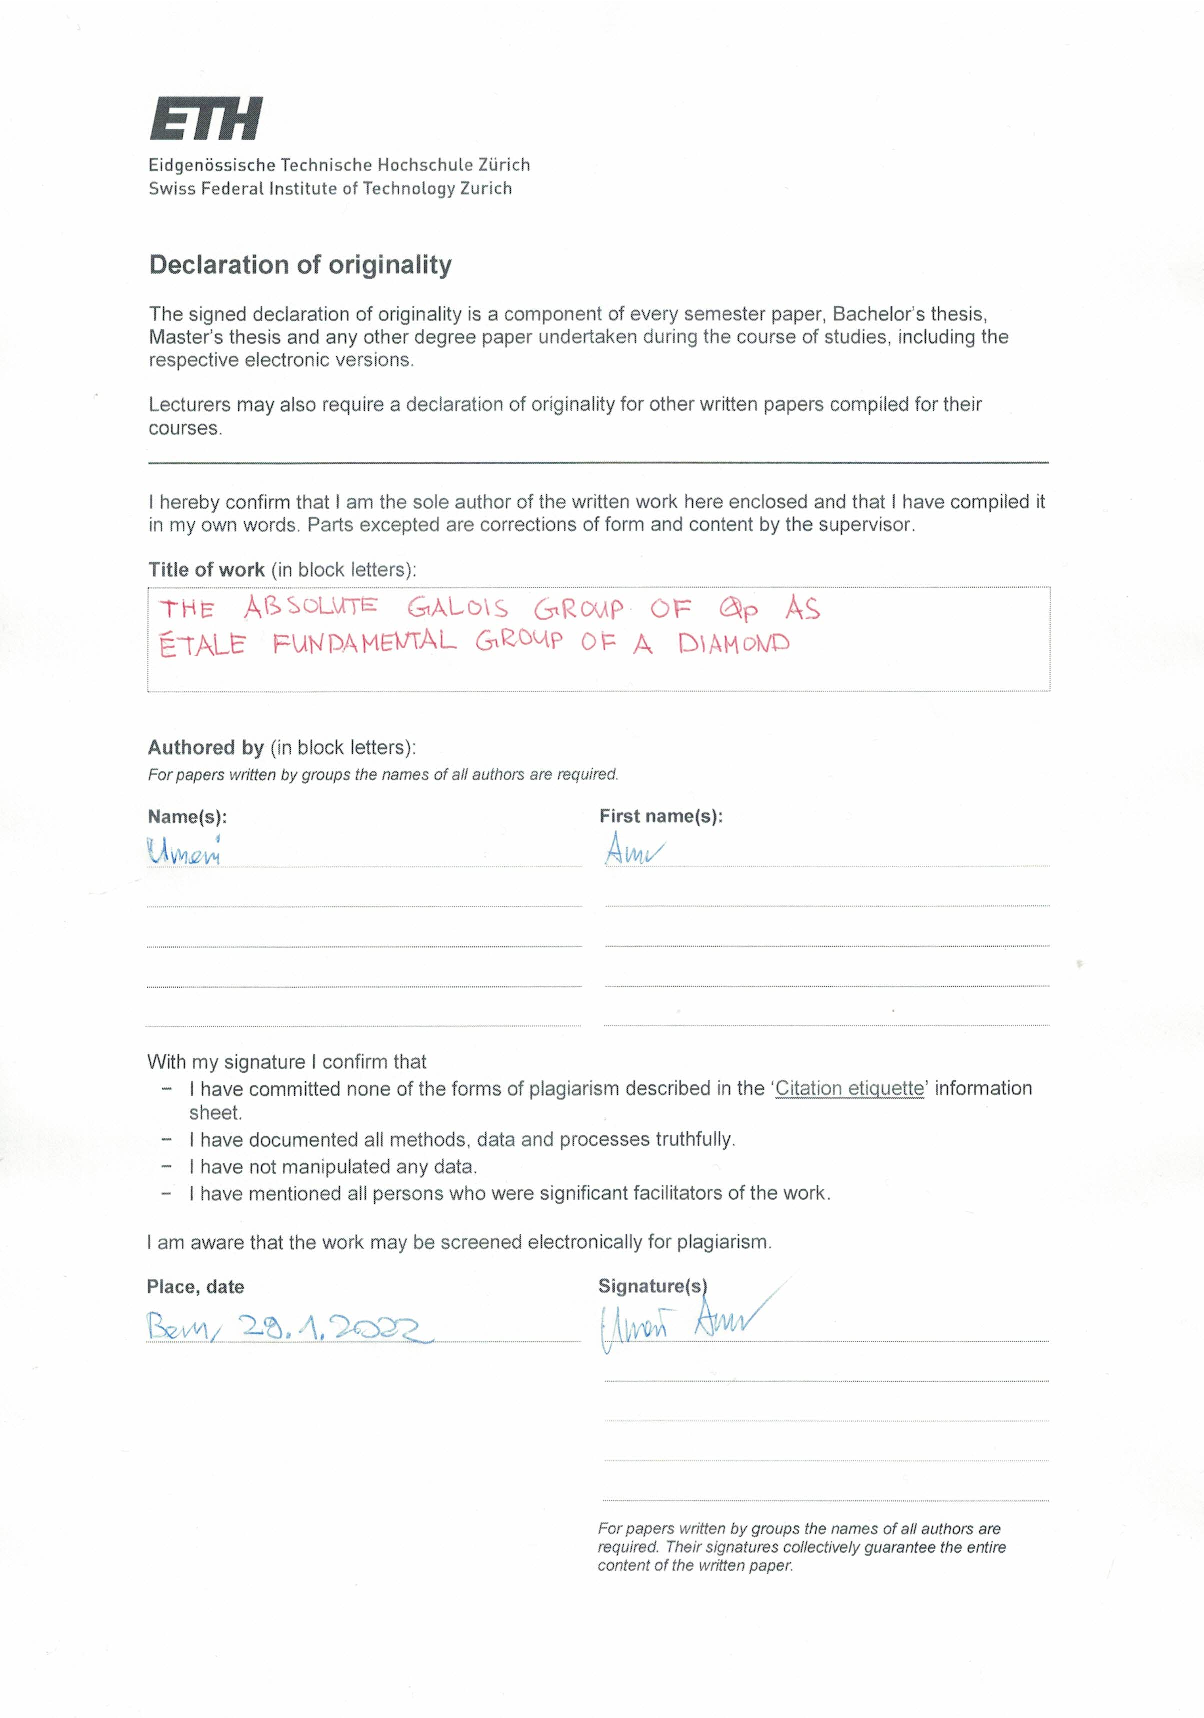
\includepdf{content/More/declaration_of_originality.pdf}
\end{document}
